% !TEX root = ./CA_solution.tex
%%%%%%%%%%%%%%%%%%%%%%%%%%%%%%%%%%%%%%%%%%%%%%%%%%
%%%%%%%%%%%%%%%%%%%%% preamble %%%%%%%%%%%%%%%%%%%
%%%%%%%%%%%%%%%%%%%%%%%%%%%%%%%%%%%%%%%%%%%%%%%%%%
%\documentclass[11pt,twoside]{book}
%=== [salt] 12p로 변경함
\documentclass[12pt,twoside]{book}
\usepackage[mono=false]{libertine} % new linux font, ignore mono

%=== [salt] 한글 tex 을 위한 패키지 추가 ===
\usepackage{kotex}

\usepackage{luatex85}

%==[salt] 수식에서 지워지는 항 표시하기
\usepackage{cancel}  


\usepackage{amsmath,amsthm,amssymb,mathrsfs,amsfonts,dsfont}
\usepackage{epsfig,graphicx}
\usepackage{tabularx}
\usepackage{blkarray}
\usepackage{slashed}
\usepackage{color}
\usepackage{listings}
\usepackage{caption}
% \usepackage{fullpage}
\usepackage{lipsum} % provides dummy text for testing
\usepackage[toc,title,titletoc,header]{appendix}
\usepackage{minitoc}
\usepackage{color}
\usepackage{multicol} % two-col ToC
\usepackage{multirow} % ===[salt]
\usepackage{bm}
\usepackage{imakeidx} % before hyperref
\usepackage{hyperref}
% link colors settings
\hypersetup{
    colorlinks=true,
    citecolor=magenta,
    linkcolor=blue,
    filecolor=green,      
    urlcolor=cyan,
    % hypertexnames=false,
}
\usepackage[capitalise]{cleveref}
\usepackage{subcaption}
\usepackage{enumitem}
\usepackage{mathtools}
\usepackage{physics}
\usepackage[linesnumbered,ruled,vlined,algosection]{algorithm2e}
\SetCommentSty{textsf}
\usepackage{epigraph}
\epigraphwidth=1.0\linewidth
\epigraphrule=0pt

% adjust margin
\usepackage[margin=2.3cm]{geometry}
\headheight13.6pt

%==============================
%=== [salt] 아래는 thmtools로 ``정리(Theorem)'' 스타일을 마음대로 만들때 사용함
%=== [salt] 관련 문서: thmtools-manual.pdf
%%%%%%%%%%%%%%%% thmtools %%%%%%%%%%%%%%%%%%%%%
\usepackage{thmtools}
\declaretheorem[numberwithin=chapter]{theorem}
\declaretheorem[numberwithin=chapter]{axiom}
\declaretheorem[numberwithin=chapter]{lemma}
\declaretheorem[numberwithin=chapter]{proposition}
\declaretheorem[numberwithin=chapter]{claim}
\declaretheorem[numberwithin=chapter]{conjecture}
\declaretheorem[sibling=theorem]{corollary}
\declaretheorem[numberwithin=chapter, style=definition]{definition}
\declaretheorem[numberwithin=chapter, style=definition]{problem}
\declaretheorem[numberwithin=chapter, style=definition]{example}
\declaretheorem[numberwithin=chapter, style=definition]{exercise}
\declaretheorem[numberwithin=chapter, style=definition]{observation}
\declaretheorem[numberwithin=chapter, style=definition]{fact}
\declaretheorem[numberwithin=chapter, style=definition]{construction}
\declaretheorem[numberwithin=chapter, style=definition]{remark}
\declaretheorem[numberwithin=chapter, style=remark]{question}
%==============================
\declaretheorem[numberwithin=chapter, style=definition, title=정리]{salt_theorem}
\declaretheorem[numberwithin=chapter, style=definition, title=보조정리]{salt_lemma}
\declaretheorem[numberwithin=chapter, style=definition, title=따름정리]{salt_corollary}
\declaretheorem[numberwithin=chapter, style=definition, title=정의]{salt_definition}
\declaretheorem[numberwithin=chapter, style=definition, title=예제]{salt_example}
\declaretheorem[numberwithin=chapter, style=definition, title=연습문제]{salt_exercise}
\declaretheorem[numberwithin=chapter, style=definition, title=명제]{salt_prop}
\declaretheorem[numberwithin=chapter, style=definition, title=참고]{salt_remark}
\declaretheorem[numberwithin=chapter, style=definition, title=추측]{salt_conjecture}
%%%%%%%%%%%%%%%% thmtools %%%%%%%%%%%%%%%%%%%%%
%==============================
%=== [salt] 수식번호 넣는 법
%\numberwithin{equation}{section}
\numberwithin{equation}{chapter}
\numberwithin{figure}{chapter}

\usepackage{changepage}
\newenvironment{solution}
    {\renewcommand\qedsymbol{$\square$}\color{blue}\begin{adjustwidth}{0em}{2em}\begin{proof}[\textit Solution.~]}
    {\end{proof}\end{adjustwidth}}

%%%%%%%%%%%%%%%% index %%%%%%%%%%%%%%%%%%%%%
\begin{filecontents}{index.ist}
% https://tex.stackexchange.com/questions/65247/index-with-an-initial-letter-of-the-group
headings_flag 1
heading_prefix "{\\centering\\large \\textbf{"
heading_suffix "}}\\nopagebreak\n"
delim_0 "\\nobreak\\dotfill"
\end{filecontents}
\newcommand{\myindex}[1]{\index{#1} \emph{#1}}
\makeindex[columns=3, intoc, title=Alphabetical Index, options= -s index.ist]
%%%%%%%%%%%%%%%% index %%%%%%%%%%%%%%%%%%%%%

%%%%%%%%%%%%%%%% ToC %%%%%%%%%%%%%%%%%%%%%
% Link Chapter title to ToC: https://tex.stackexchange.com/questions/32495/linking-the-section-text-to-the-toc
\usepackage[explicit]{titlesec}
\titleformat{\chapter}[display]
  {\normalfont\huge\bfseries}{\chaptertitlename\ {\thechapter}}{20pt}{\hyperlink{chap-\thechapter}{\Huge#1}
\addtocontents{toc}{\protect\hypertarget{chap-\thechapter}{}}}
\titleformat{name=\chapter,numberless}
  {\normalfont\huge\bfseries}{}{-20pt}{\Huge#1}

%%%%%%%%%%%%%%%%%%% fancyhdr %%%%%%%%%%%%%%%%%
\usepackage{fancyhdr}
\pagestyle{fancy} % enable fancy page style
\renewcommand{\headrulewidth}{0.0pt} % comment if you want the rule
\fancyhf{} % clear header and footer
\fancyhead[lo,le]{\leftmark}
\fancyhead[re,ro]{\rightmark}
\fancyfoot[CE,CO]{\hyperref[toc-contents]{\thepage}}

% https://tex.stackexchange.com/questions/550520/making-each-page-number-link-back-to-beginning-of-chapter-or-section
\makeatletter
\def\chaptermark#1{\markboth{\protect\hyper@linkstart{link}{\@currentHref}{Chapter \thechapter ~ #1}\protect\hyper@linkend}{}}
\def\sectionmark#1{\markright{\protect\hyper@linkstart{link}{\@currentHref}{\thesection ~ #1}\protect\hyper@linkend}}
\makeatother
%%%%%%%%%%%%%%%%%%% fancyhdr %%%%%%%%%%%%%%%%%


%%%%%%%%%%%%%%%%%%% biblatex %%%%%%%%%%%%%%%%%
\usepackage[doi=false,url=false,isbn=false,style=alphabetic,backend=biber,backref=true]{biblatex}
\addbibresource{bib.bib}

\newbibmacro{string+doiurlisbn}[1]{%
  \iffieldundef{doi}{%
    \iffieldundef{url}{%
      \iffieldundef{isbn}{%
        \iffieldundef{issn}{%
          #1%
        }{%
          \href{http://books.google.com/books?vid=ISSN\thefield{issn}}{#1}%
        }%
      }{%
        \href{http://books.google.com/books?vid=ISBN\thefield{isbn}}{#1}%
      }%
    }{%
      \href{\thefield{url}}{#1}%
    }%
  }{%
    \href{http://dx.doi.org/\thefield{doi}}{#1}%
  }%
}

% https://tex.stackexchange.com/questions/94089/remove-quotes-from-inbook-reference-title-with-biblatex
\DeclareFieldFormat[article,incollection,inproceedings,book,misc]{title}{\usebibmacro{string+doiurlisbn}{\mkbibemph{#1}}}
% https://tex.stackexchange.com/questions/454672/biblatex-journal-name-non-italic
\DeclareFieldFormat{journaltitle}{#1\isdot}
\DeclareFieldFormat{booktitle}{#1\isdot}
% https://tex.stackexchange.com/questions/10682/suppress-in-biblatex
\renewbibmacro{in:}{}
% add video field: https://tex.stackexchange.com/questions/111846/biblatex-2-custom-fields-only-one-is-working
\DeclareSourcemap{
    \maps[datatype=bibtex]{
      \map{
        \step[fieldsource=video]
        \step[fieldset=usera,origfieldval]
    }
  }
}
\DeclareFieldFormat{usera}{\href{#1}{\textsc{Online video}}}
\AtEveryBibitem{
    \csappto{blx@bbx@\thefield{entrytype}}{% put at end of entry
        \iffieldundef{usera}{}{\space \printfield{usera}}
    }
}
%%%%%%%%%%%%%%%%%%% biblatex %%%%%%%%%%%%%%%%%

%%%%%%%%%%%%%%%%%%%%% glossaries %%%%%%%%%%%%%%%%%
%% !TEX root = ./notes_template.tex
% \usepackage[style=super]{glossaries}
% https://www.overleaf.com/learn/latex/Glossaries
\usepackage[style=super,toc,acronym]{glossaries}
\setlength{\glsdescwidth}{1\linewidth}
\makeglossaries

\renewcommand\glossaryname{List of Abbreviations and Symbols}

\newglossaryentry{Q2}{name={$Q_2(f)$},
%sort=Q2,
description={Two-side (bounded) error quantum query complexity}}

\newglossaryentry{real_number}{name={$\mathbb{R}$},description={Real number}}

% \newglossaryentry{gcd}{name={gcd},description={greatest common divisor}}

\newacronym{gcd}{GCD}{Greatest Common Divisor}


\newglossaryentry{svm}{name={SVM},description={Support Vector Machine}}

\newglossaryentry{gd}{name={GD},description={Gradient Descent}}

\newglossaryentry{qft}{name={QFT},description={Quantum Field Theory}}

\newglossaryentry{qm}{name={QM},description={Quantum Mechanics}}

\newglossaryentry{v}{name={$\vec{v}$},description={a vector}}

% physics
\newglossaryentry{hamiltonian}{name={$\hat{H}$},description={Hamiltonian}}

\newglossaryentry{lagrangian}{name={$L$},description={Lagrangian}}
%%%%%%%%%%%%%%%%%%%%% glossaries %%%%%%%%%%%%%%%%%

%%%%%%%%%%%%%%%%%%%%% glossaries-extra %%%%%%%%%%%%%%%%%
% \usepackage[record,abbreviations,symbols,stylemods={list,tree,mcols}]{glossaries-extra}
%%%%%%%%%%%%%%%%%%%%% glossaries-extra %%%%%%%%%%%%%%%%%


%% !TEX root = ./notes_template.tex

%%%%%%%%%%%%%%%%%%%%%%%%%%%%%%%%%%%%
%%%%%%%%%%%%%%%%%%%%%%%%%%%%%%%%%%%%
% math
\let\iff\relax
\newcommand{\iff}{\text{ iff }}
\newcommand{\OPT}{\textup{OPT}}

% physics
\newcommand{\acreation}{a^\dagger}



%%%%%%%%%%%%%%%%%%%%%%%%%%%%%%%%%%%%%%%%%%%%%%%%%%
%%%%%%%%%%%%%%%% begin of document %%%%%%%%%%%%%%%
%%%%%%%%%%%%%%%%%%%%%%%%%%%%%%%%%%%%%%%%%%%%%%%%%%


%=== [salt] 줄 간격을 읽기 좋게 만든다.
% 계산공식: 줄간격 = \baselinestretch x \baselineskip
\renewcommand{\baselinestretch}{1.3}
%\setlength{\baselineskip}{30pt}
\setlength{\parskip}{5pt}
\setlength{\itemsep}{0pt}
%\setlength{\parindent}{20pt}

%=== [salt] 수식의 줄간격 조절 수식($$ $$)에서 유효함
\everydisplay\expandafter{\the\everydisplay\def\baselinestretch{1.0}\selectfont}
\allowdisplaybreaks

%=== [salt] 기호( :) 간격을 줄인다 --> 너무 줄어든다!
%\DeclareMathSymbol{:}{\mathord}{operators}{"3A}

%=== [salt] 추가 정의들
\def\disp{\displaystyle}
\def\dfrac{\disp\frac}
\def\dint{\disp\int}
\newcommand{\Log}{\mathop{\mathrm{Log}}}
\newcommand{\Arg}{\mathop{\mathrm{Arg}}}
\newcommand{\Hol}{\mathop{\mathrm{Hol}}}
\newcommand{\Har}{\mathop{\mathrm{Har}}}
\newcommand{\res}{\mathop{\mathrm{res}}}
\newcommand{\sgn}{\mathop{\mathrm{sgn}}}
\def\Sum{\sum\limits}
\def\Lim{\lim\limits}
\def\bs{\boldsymbol }

\def\figurename{그림}
%\renewcommand{\thefigure}{\arabic{section}-\arabic{figure}}
\begin{document}

%==============================
%=== [salt] 책 표지 만들기 시작
%\title{\bf {\huge 빠르게 이해하는 복소해석학}\\ A Friendly Approach to Complex Analysis}
%\title{\bf {\huge 친구처럼 가까운 복소해석학 여행}\\ A Friendly Approach to Complex Analysis}
\title{\bf {\huge 복소해석학 연습문제 풀이}\\ A Friendly Approach to Complex Analysis}
\author{염용진,허재성 譯}
\date{Update on \today}
\maketitle

%=== [salt] 이 카운트들은 뭘까??? 
%\setcounter{tocdepth}{2}
%=== [salt]  각 챕터시작할 때 \minitoc 에서 사용하는 것 
\setcounter{minitocdepth}{1} 

%=== [salt]  목차를 한글로 쓰기
%\renewcommand{\contentsname}{목 차}
%\tableofcontents
    
    
%=== [salt] 2 컬럼으로 목차들 만들기 (굳이?)
%\begin{multicols}{2}
%    \dominitoc% Initialization
%    \adjustmtc[2]% chp number shift for mini-toc
%   \tableofcontents
%    \label{toc-contents}
%\end{multicols}
%
%	\listoffigures
%	% \listoftables
%\begin{multicols}{2}
%	\listoftheorems[ignoreall,show={theorem}]
%\end{multicols}
%
%	\renewcommand{\listtheoremname}{List of Definitions}
%\begin{multicols}{2}
%	\listoftheorems[ignoreall,show={definition}]
%\end{multicols}
%=== [salt] 2 컬럼으로 목차들 만들기끝 
%==============================

	% \printglossaries
	% \printglossary[type=\acronymtype]
	%=== [salt]  기본으로 되어 있었으나 비활성화함 \printglossary
	 %\printglossary[title=List of terms, toctitle=List of terms]

	% bib2gls
	% \printunsrtglossaries % print all types
	% \printunsrtglossary[type={abbreviations},title=List of Abbreviations,style=listgroup]
	% \printunsrtglossary[type={abbreviations},title=List of Abbreviations,style=listhypergroup] % doesn't work
	% \printunsrtglossary[type={symbols},title=List of Symbols,style=listgroup]
	% \printunsrtglossary % main entry

%%%%%%%%%%%%%%%Content%%%%%%%%%%%%%%%
% \mainmatter % separat the number of toc and mainmatter


%===[salt] 0장, 1장
% !TEX root = ./CA_solution.tex

\chapter*{연습문제 풀이}

\section*{머리말 - 연습문제 풀이}

\subsection*{연습문제 \ref{ex-0-1}}

$0$에서 $f'$의 미분이 존재하고 그 값이 $L$이라고 가정하자.
$\epsilon:=1>0$으로 잡으면, $0<|x-0|<\delta$이면
\[
\left| \dfrac{f'(x) - f'(0)}{x-0} - L\right| <\epsilon
\]
을 만족하는 $\delta>0$가 존재한다.
특히 $x:=\delta/2$로 잡으면
$0<|x-0| = \delta/2 < \delta$이므로
\begin{equation} \label{eq-5-5}
\left| \dfrac{f'(x) - f'(0)}{x-0} - L\right|
= \left| \dfrac{2(\delta/2) - 0}{(\delta/2)-0} - L\right| 
= |2-L| < \epsilon.
\end{equation}
한편 $x:=-\delta/2$로 잡아도
$0<|x-0| = \delta/2 < \delta$이므로
\begin{equation} \label{eq-5-6}
\left| \dfrac{f'(x) - f'(0)}{x-0} - L\right|
= \left| \dfrac{-2(-\delta/2) - 0}{(-\delta/2)-0} - L\right| 
= |2+L| < \epsilon.
\end{equation}
식 \eqref{eq-5-5}와 \eqref{eq-5-6}으로부터
실수 절대값에 대한 삼각부등식을  이용하면
\[
4 = |2+L+2-L| \le |2+L| + |2-L|
<\epsilon + \epsilon = 2\epsilon = 2
\]
가 되어 모순이다.
따라서 $f'$은 $0$에서 미분이 불가능하다.

\section*{1장 - 연습문제 풀이}

\subsection*{연습문제 \ref{ex-1-1}}

$(x,y) \ne 0$이므로, 
$x$, $y$ 중 적어도 하나는 $0$이 아니다.
따라서 $x^2+y^2\ne 0$이고,
\[
\left( \dfrac x{x^2+y^2}, \dfrac{-y}{x^2+y^2} \right) \in \mathbb R^2.
\]
또한,
\begin{align*}
(x,y) \cdot & \left( \dfrac x{x^2+y^2}, \dfrac{-y}{x^2+y^2} \right) \\
&=\left( x\cdot \dfrac x{x^2+y^2} - y\cdot \left( \dfrac{-y}{x^2+y^2} \right),
x\cdot \left(\dfrac{-y}{x^2+y^2}\right) + y\cdot  \dfrac{x}{x^2+y^2} \right) \\
&= \left( \dfrac{x^2+y^2}{x^2+y^2}, \dfrac{-xy + xy}{x^2+y^2} \right) = (1,0).
\end{align*}
따라서 $(x,y) \ne(0,0)$에 대하여
$
(x,y)^{-1} = \left(\dfrac x{x^2+y^2}, \dfrac{-y}{x^2+y^2} \right)
$이다.

\subsection*{연습문제 \ref{ex-1-2}}

$\theta \in \left(-\dfrac{\pi}2, \dfrac\pi2 \right)$이므로,
$\tan \theta \in \mathbb R$이고,

\begin{align*}
\dfrac1{1-i\tan\theta}
&= \dfrac1{1^2+(\tan\theta)^2} 
+ i\left( \dfrac{\tan\theta}{1^2 + (\tan\theta)^2} \right) \\
&= \dfrac{(\cos\theta)^2}{(\cos\theta)^2 + (\sin\theta)^2}
+ i\left( \dfrac{\dfrac{\sin\theta}{\cos\theta}\cdot(\cos\theta)^2}
{(\cos\theta)^2 + (\sin\theta)^2} \right) \\
&= \dfrac{(\cos\theta)^2}1 + i \dfrac{(\sin\theta)(\cos\theta)}1
= (\cos\theta)^2 + i(\sin\theta)(\cos\theta).
\end{align*}
따라서
\begin{align*}
\dfrac{1+i\tan\theta}{1-i\tan\theta}
&= (1+i\tan\theta)( (\cos\theta)^2 + i(\sin\theta)(\cos\theta) ) \\
&= (\cos\theta)^2 - \dfrac{\sin\theta}{\cos\theta} \cdot
(\sin\theta)(\cos\theta) \\
&\quad\quad + \left(
(\sin\theta)(\cos\theta) + \dfrac{\sin\theta}{\cos\theta} \cdot (\cos\theta)^2
\right) \\
&= (\cos\theta)^2 - (\sin\theta)^2 + i2(\sin\theta)(\cos\theta)
= \cos(2\theta) + i\sin(2\theta).
\end{align*}

\subsection*{연습문제 \ref{ex-1-3}}

$P\subset \mathbb C$가 $\mathbb C$의 양의 부분집합이라고 하자.
그러면, $i\ne0$이므로 조건 (P3)에 의해
$i\in P$이거나 ($i\ne P$이고 $-i\in P$)이다.
조건 (P2)에서
\begin{equation}\label{eq-5-7}
-1 = i\cdot i = (-i)\cdot (-i) \in P
\end{equation}
이고, 다시 (P2)에서
\begin{equation}\label{eq-5-8}
1 = (-1)\cdot(-1) \in P
\end{equation}
가 된다. 
그런데 $1\ne0$이고
$x=1$이라고 하면 (P3)에서
\eqref{eq-5-7}, \eqref{eq-5-8}\은 동시에 만족될 수 없기에 모순이다.

\subsection*{연습문제 \ref{ex-1-4}}

아래 그림 \ref{fig-5-2}\와 같다.

\begin{figure}[h!]
\begin{center}
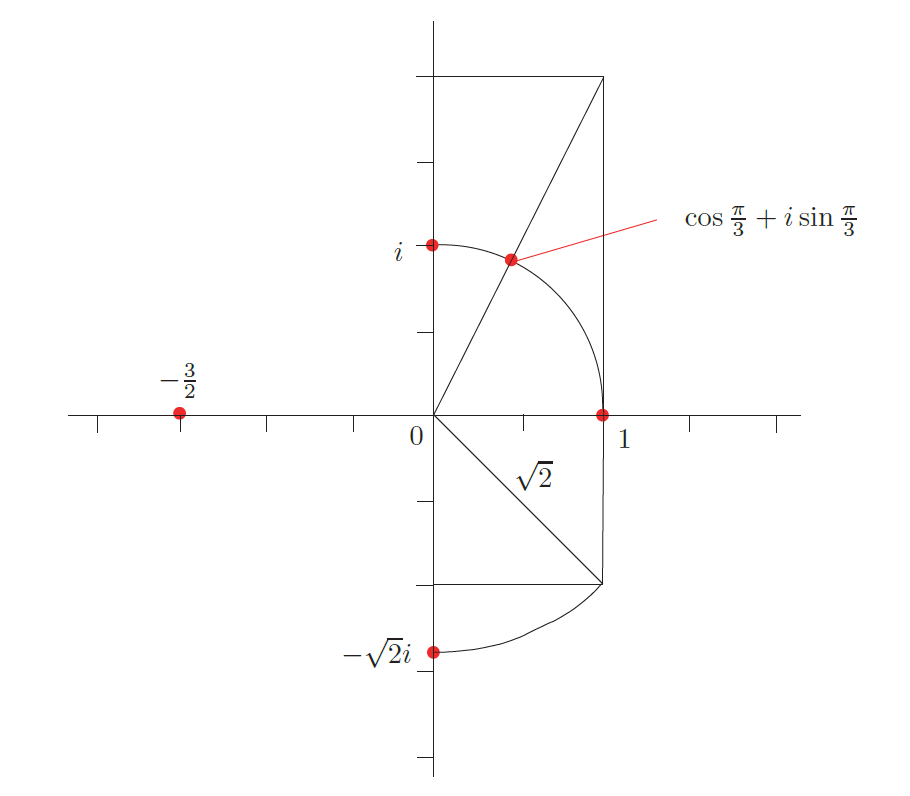
\includegraphics[width=0.7\textwidth]{./figs/fig-5-2}
\end{center}
\caption{복소수 $0$, $1$, $-3/2$, $i$, $-\sqrt{2}i$,
$\cos\dfrac\pi3 + i\sin\dfrac\pi3$의 위치}
\label{fig-5-2}
\end{figure}

\subsection*{연습문제 \ref{ex-1-5}}

$\theta\in\mathbb R$에 대하여
$(\cos\theta + i\sin\theta)^3 = \cos(3\theta) + i\sin(3\theta)$이다.
\begin{align*}
(\cos\theta + i\sin\theta)^3 
&= (\cos\theta + i\sin\theta)\left(
(\cos\theta)^2 - (\sin\theta)^2 + i2(\cos\theta)(\sin\theta) \right) \\
&= (\cos\theta)\left( (\cos\theta)^2 - (\sin\theta)^2 \right)
- (\sin\theta)2(\cos\theta)(\sin\theta)  \\
&\quad\quad + i(\ \cdots\ ).
\end{align*}
따라서 양변의 실수부가 같다는 것을 이용하면,
\begin{align*}
\cos(3\theta) &= \Re((\cos\theta + i\sin\theta)) \\
&=(\cos\theta)\left( (\cos\theta)^2 - (\sin\theta)^2 \right)
- 2(\cos\theta)(\sin\theta)^2 \\
&= (\cos\theta)\left( (\cos\theta)^2 - 1 + (\cos\theta)^2 \right)
- 2(\cos\theta)(1-\cos\theta)^2 \\
&= (\cos\theta)^3 - \cos\theta  + (\cos\theta)^3 - 2\cos\theta + 2(\cos\theta)^3 \\
&= 4(\cos\theta)^3 - 3\cos\theta
\end{align*}
다른 방법으로, 이항정리 공식
$(a+b)^n = \Sum_{k=0}^n \disp{n \choose k} a^kb^{n-k}$이
복소수 $a,b \in \mathbb C$와 자연수 $n\in \mathbb N$에 대하여
성립한다는 것을 이용하면,
\begin{align*}
\cos(3\theta) &= \Re((\cos\theta + i\sin\theta)) \\
&= \Re ( (\cos\theta)^3 + 3(\cos\theta)^2(i\sin\theta) 
+ 3(\cos\theta)(i\sin\theta)^2 + (i\sin\theta)^3) \\
&= (\cos\theta)^3 - 3(\cos\theta)(\sin\theta)^2 \\
&= 4(\cos\theta)^3 - 3\cos\theta.
\end{align*}

\subsection*{연습문제 \ref{ex-1-6}}

$1+i = \sqrt{2}\left(\dfrac1{\sqrt{2}} + i\dfrac1{\sqrt{2}}\right)
= \sqrt{2}\left( \cos\dfrac\pi4 + i\sin \dfrac\pi4 \right)$로 쓸 수 있다.
따라서,
\begin{align*}
(1+i)^{10}
&= (\sqrt{2})^{10} \left( \cos\dfrac\pi4 + i\sin \dfrac\pi4 \right)^{10}
= 2^5 \left( \cos\left(10\cdot \dfrac\pi4\right) 
+ i\sin \left(10\cdot \dfrac\pi4\right) \right) \\
&= 32 \left( \cos\left(2\pi+\dfrac\pi2\right) 
+ i\sin \left(2\pi+\dfrac\pi2\right) \right) \\
&=32 \left( \cos\left(\dfrac\pi2\right) + i\sin \left(\dfrac\pi2\right) \right) 
= 32(0+i\cdot 1) = 32i.
\end{align*}

\subsection*{연습문제 \ref{ex-1-7}}

$2+i$가 실수축의 양의 방향과 이루는 각도는 $\tan^{-1}(1/2)$이고
$3+i$가 실수축의 양의 방향과 이루는 각도는 $\tan^{-1}(1/3)$이다.
따라서, $(2+i)(3+i)$가 실수축의 양의 방향과 이루는 각도는 
$\tan^{-1}(1/2) + \tan^{-1}(1/3)$이다.
한편,
\[
(2+i)(3+i) = 6 - 1 + i(2+3) = 5 + 5i
\]
이므로 $(2+i)(3+i)$가  실수축의 양의 방향과 이루는 각도는
\[
\tan^{-1} (5/5) = \tan^{-1} 1 = \pi/4
\]
이다. 결론적으로, 
$\dfrac\pi4 = \tan^{-1}\dfrac12 + \tan^{-1}\dfrac13$이다.

\subsection*{연습문제 \ref{ex-1-8}}

정삼각형의 꼭지점  $A$, $B$, $C$의 위치가 
반시계방향의 순서로 복소수 $z_A$, $z_B$, $z_C$에 있다고 하자.
$\ell(AC) = \ell(AB)$이고 $\angle CAB=\pi/3$이므로,
\begin{equation}\label{eq-5-9}
z_C - z_A = \left( \cos\dfrac\pi3 + i\sin\dfrac\pi3 \right)(z_B - z_A).
\end{equation}
귀류법을 쓰기위해 $p,q,m,n\in\mathbb Z$가 
\[
z_C - z_A = p+iq, \quad
z_B - z_A = m+in
\]
을 만족한다고  하자.
그러면, 식 \eqref{eq-5-9}에서
$p+iq = \left(\dfrac12 + \dfrac{\sqrt{3}}2i\right)(m+in)$을 다시 쓰면,
\begin{align}
p &= \dfrac m2 - \dfrac{\sqrt{3}}2n, \label{eq-5-10} \\
q &= \dfrac{m\sqrt{3}}2 + \dfrac n2. \label{eq-5-11}
\end{align}
식 \eqref{eq-5-10}에 $-n$을 곱하고,
식 \eqref{eq-5-11}에 $m$을 곱하여 더하면,
\[
qm - pn = \dfrac{\sqrt{3}}2 (m^2 + n^2)
\]
을 얻는다.
그런데 $m^2+n^2 \ne0$이므로 ($z_B \ne z_A$이므로),
\[
\sqrt{3} = \dfrac{2(qm-pn)}{m^2+n^2} \in \mathbb Q
\]
를 얻어 모순이 생긴다.

\subsection*{연습문제 \ref{ex-1-9}}

$-1 = 1 \cdot (\cos \pi + i \sin \pi)$로 쓸 수 있다.
$w = \rho(\cos\alpha + i\sin\alpha)$가 
\[
w^4 = \rho^4(\cos(4\alpha) + i\sin(4\alpha)) = 1 \cdot (\cos \pi + i \sin \pi)
\]
를 만족해야 하므로,
$\rho^4 = 1$에서 $\rho=1$이다.
또한, $4\alpha \in \{ \pi, \pi\pm2\pi, \pi\pm4\pi, \ldots\}$에서
\[
\alpha \in \left\{ \dfrac\pi4, \dfrac\pi4\pm\dfrac\pi2, \dfrac\pi4\pm\pi,\ldots
\right\}.
\]
따라서 $ w = \rho(\cos\alpha + i\sin\alpha) = 1\cdot((\cos\alpha + i\sin\alpha) $는
다음 집합에 속한다.
\begin{align*}
&\left\{ \cos\dfrac\pi4+i\sin\dfrac\pi4, \cos\dfrac{3\pi}4+i\sin\dfrac{3\pi}4, 
\cos\dfrac{5\pi}4+i\sin\dfrac{5\pi}4, \cos\dfrac{7\pi}4+i\sin\dfrac{7\pi}4
\right\} \\
&\qquad\quad\quad = \left\{ \dfrac{1+i}{\sqrt{2}},  \dfrac{-1+i}{\sqrt{2}},
 \dfrac{-1-i}{\sqrt{2}},  \dfrac{1-i}{\sqrt{2}} \right\}.
\end{align*}

네 개의 해를 복소평면에 그려보면 그림 \ref{fig-5-3}\과 같다.

\begin{figure}[h!]
\begin{center}
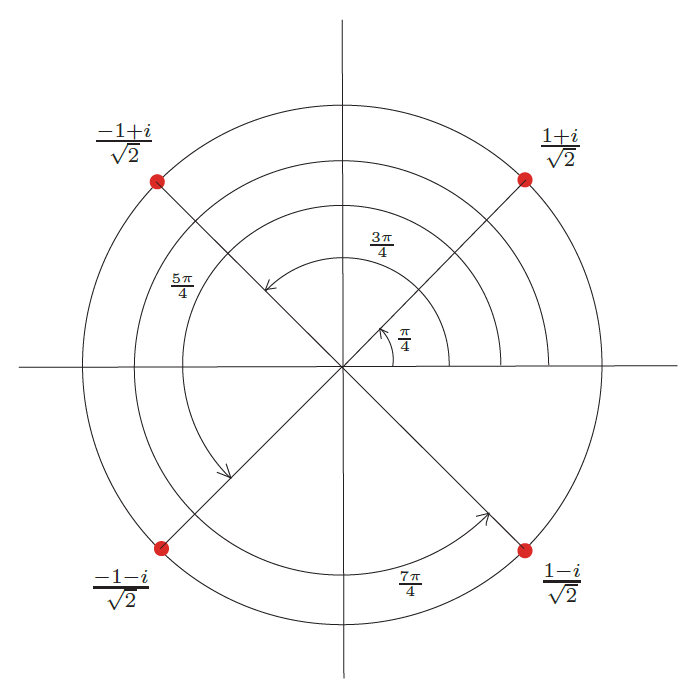
\includegraphics[width=0.6\textwidth]{./figs/fig-5-3}
\end{center}
\caption{$w^4=-1$을 만족하는 복소수 $w$의 위치}
\label{fig-5-3}
\end{figure}

\subsection*{연습문제 \ref{ex-1-10}}

방정식으로부터
\[
0=z^6 -z^3-2 = (z^3)^2 -2z^3 +z^3 -2 = (z^3-2)(z^3+1)
\]
이므로
$z^3=2$ 또는 $z^3=-1$이다.
$z^3=2$를 만족하는 해를 구하면
\[
z\in \left\{ \sqrt[3]{2} \left( \cos\dfrac{2\pi}3 + i\sin\dfrac{2\pi}3\right),
\sqrt[3]{2} \left( \cos\dfrac{4\pi}3 + i\sin\dfrac{4\pi}3\right), 
\sqrt[3]{2} \right\}
\]
로부터 
\[
z\in \left\{ \sqrt[3]{2} \left( - \dfrac12+ i\dfrac{\sqrt{3}}2\right),
\sqrt[3]{2} \left( -\dfrac12 - i\dfrac{\sqrt{3}}2\right), 
\sqrt[3]{2} \right\}
\]
이다. 한편, $z^3=-1$의 해는
\[
z\in\left\{ \cos\dfrac\pi3 + i\sin\dfrac\pi3, \cos\pi + i\sin\pi,
\cos\dfrac{5\pi}3 + i\sin\dfrac{5\pi}3 \right\}
\]
로부터 
\[
z\in \left\{ \dfrac12+ i\dfrac{\sqrt{3}}2, -1,
\dfrac12 - i\dfrac{\sqrt{3}}2 \right\}
\]
이다. 결론적으로
$z^6 - z^3-2=0$일 필요충분조건은 [$z^3=2$ 또는 $z^3=-1$]이다.
즉,
\begin{align*}
z\in & \left\{ \sqrt[3]{2} \left( - \dfrac12+ i\dfrac{\sqrt{3}}2\right),
\sqrt[3]{2} \left( -\dfrac12 - i\dfrac{\sqrt{3}}2\right), 
\sqrt[3]{2} \right\}\\
&\bigcup \left\{ \dfrac12+ i\dfrac{\sqrt{3}}2, -1,
\dfrac12 - i\dfrac{\sqrt{3}}2 \right\}.
\end{align*}
따라서 구하는 해는
\[
z\in \left\{ \sqrt[3]{2} \left( - \dfrac12+ i\dfrac{\sqrt{3}}2\right),
\sqrt[3]{2} \left( -\dfrac12 - i\dfrac{\sqrt{3}}2\right), 
\sqrt[3]{2},
\dfrac12+ i\dfrac{\sqrt{3}}2, -1,
\dfrac12 - i\dfrac{\sqrt{3}}2 \right\}.
\]

\subsection*{연습문제 \ref{ex-1-11}}

$\omega^3=1$을 만족하는 $\omega\in\mathbb C \setminus \mathbb R$을 생각하자.
그러면, $(\omega-1)(\omega^2+\omega+1)=0$이고,
$\omega\ne1$이므로 $\omega^2+\omega+1=0$이다.
따라서,
\begin{align*}
((b-a)\omega &+(b-c))((b-a)\omega^2+b-c) \\
&= (b-a)^2\omega^3 + (b-a)(b-c)(-1) + (b-c)^2 \\
&= (b-a)^2\cdot 1 + (b-a)(b-c)(-1)  + (b-c)^2 \\
&= (b-a)(b-a-b+c) + (b-c)^2 \\
&=(bc-ca-ab+a^2+b^2-2bc+c^2 \\
&= a^2+b^2+c^2 -ab - bc - ca = 0.
\end{align*}
따라서 $(b-a)\omega = c-b$이거나 $(b-a)\omega^2 = c-a$이다.
두번째 식은 $(b-a)\omega^3 = (c-a)\omega$와 동치이므로
$(c-b)\omega = b-a$이다.
이로부터 $|b-a|=|c-b|$를 얻고
$a$와 $b$, $a$와 $c$를 잇는 두 선분의 사잇각은 $\pi/3$이다.
그림 \ref{fig-5-4}\를 참고하라.

\begin{figure}[h!]
\begin{center}
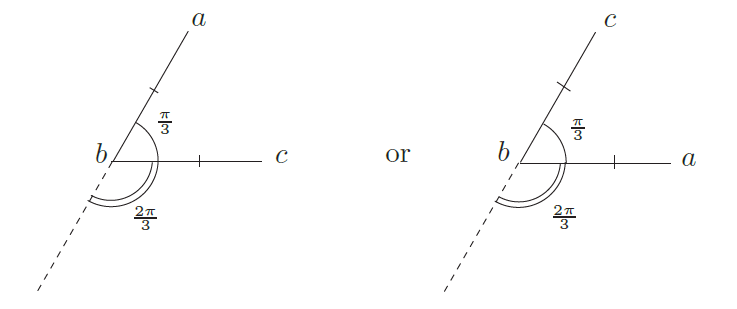
\includegraphics[width=0.6\textwidth]{./figs/fig-5-4}
\end{center}
\caption{정삼각형을 이루는 세 점 $a$, $b$, $c$}
\label{fig-5-4}
\end{figure}

두 가지 그림 모두 세 점 $a$, $b$, $c$는 정삼각형을 이룬다.
 $a$, $b$, $c$가 실수인 경우는 한점 $r\in\mathbb R$로 모이게 되어
 $a=b=c=(=r)$이 되어 실수의 경우도 원하는 결과를 얻는다.

\subsection*{연습문제 \ref{ex-1-12}}

$\omega\in\mathbb C\setminus \mathbb R$이 $\omega^3=1$을 만족한다고 하자.
$(\omega-1)(\omega^2+\omega+1)=0$이고,
$\omega\ne1$이므로 $\omega^2+\omega+1=0$이다.
또한, $1+\omega^2+\omega^4 = 1+ \omega^2 + \omega\cdot\omega^3 =
1+ \omega^2 + \omega = 0$이므로,
\[
(1+1)^{3n} + (1+\omega)^{3n} + (1+\omega^2)^{3n}
= \Sum_{k=0}^{3n} {3n \choose k} (1+\omega^k + \omega^{2k}).
\]
그런데,
\begin{align*}
(1+\omega^k + \omega^{2k})
&= \begin{cases}
1+1+1, & k\equiv 0 \mod 3, \\
1+\omega + \omega^2, & k\equiv 1 \mod 3, \\
1+\omega^2 + \omega^4,& k\equiv 2 \mod 3
\end{cases} \\
&=\begin{cases}
3, & k\equiv 0 \mod 3, \\
0, & k\equiv 1 \mod 3, \\
0, & k\equiv 2 \mod 3.
\end{cases}
\end{align*}
에서
\[
(1+1)^{3n} + (1+\omega)^{3n} + (1+\omega^2)^{3n}
= 3\cdot \left(
{3n \choose 0} + {3n \choose 3} + \cdots + {3n \choose 3n} \right).
\]
다른 방법으로 보면,
\begin{align*}
(1+1)^{3n} + (1+\omega)^{3n} + (1+\omega^2)^{3n}
&= 2^{3n} + (-\omega^2)^{3n} +  (-\omega)^{3n} \\
&= 2^{3n} + (-1)^n + (-1)^n \\
&= 2^{3n} + 2\cdot(-1)^n
\end{align*}
이므로 원하는 결과를 얻는다.

\subsection*{연습문제 \ref{ex-1-13}}

\begin{figure}[h!]
\begin{center}
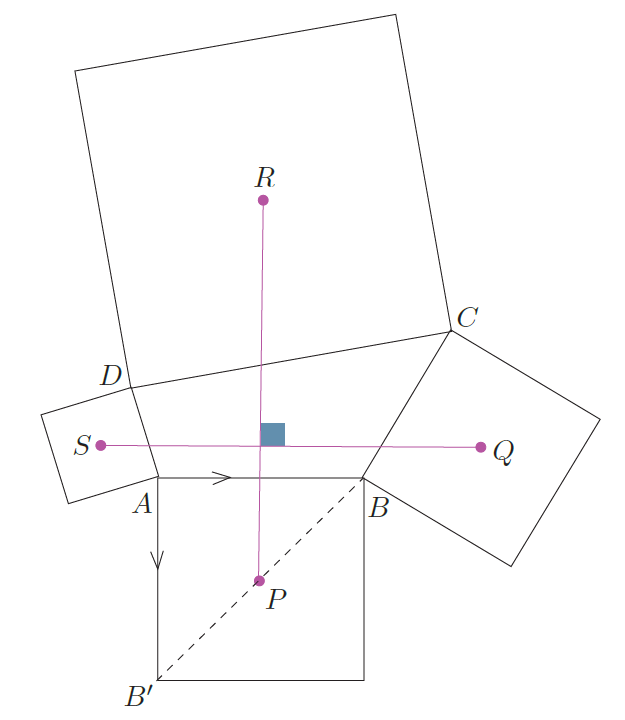
\includegraphics[width=0.6\textwidth]{./figs/fig-5-5}
\end{center}
\caption{$RP$와 $SQ$는 길이가 같고 수직으로 만난다}
\label{fig-5-5}
\end{figure}

그림 \ref{fig-5-5}\와 같이
평면위의 네 점 $A$, $B$, $C$, $D$를 복소수 $a$, $b$, $c$, $d$에 각각 대응시키자.
$AB'$은  $A$를 중심으로 하여 $AB$를 반시계방향으로 $90^\circ$회전한 것이므로
$B'$은 복소수 $a-i(b-a)$에 대응된다.
$P$는 $BB'$의 중점이므로 다음 복소수에 대응된다.
\[
\dfrac{a+b-i(b-a)}2.
\]
같은 방법으로 $Q$, $R$, $S$는 각각 다음 복소수에 대응된다.
\[
\dfrac{b+c-i(c-b)}2, \quad
\dfrac{c+d-i(d-c)}2, \quad
\dfrac{d+a-i(a-d)}2.
\]
점 $P$, $Q$, $R$, $S$에 대응되는 복소수를 각각
$p$, $q$, $r$, $s$라 하면,
\begin{align*}
i(q-s) &= i \left(
\dfrac{b+c-i(c-b)}2 - \dfrac{d+a-i(a-d)}2 \right) \\
&= \dfrac{-b+c-a+d+i(b+c-d-a)}2 \\
&= \dfrac{-a-b+i(b-a)}2 + \dfrac{c+d-i(d-c)}2 = -p+r
\end{align*}
이므로, $|q-s| = |p-r|$이 되어 $\ell(QS) = \ell(PR)$이다.
또한, $i$를 곱하는 것은 원점을 중심으로 $90^\circ$ 회전을 의미하기 때문에
$PR\perp QS$이다.

\subsection*{연습문제 \ref{ex-1-14}}

실수 $x_1, x_2, y_1, y_2$에 대하여
$z_1 = x_1 + iy_1$, $z_2 = x_2 + iy_2$라 하자.
그러면 $z_1z_2 = x_1x_2 - y_1y_2 = i(x_1y_2+y_1x_2)$이고,
\begin{align*}
|z_1z_2|^2 &=  (x_1x_2 - y_1y_2)^2 + (x_1y_2 + y_1x_2)^2 \\
&= x_1^2x_2^2 - \cancel{2x_1x_2y_1y_2} + y_1^2y_2^2
+ x_1^2y_2^2 + \cancel{2x_1y_2y_1x_2} + y_1^2x_2^2 \\
&=x_1^2(x_2^2+y_2^2) + y_1^2(y_2^2+x_2^2)
= (x_1^2+y_1^2)(x_2^2+y_2^2) \\
&= |z_1|^2|z_2|^2.
\end{align*}
$|z_1|$, $|z_2|$, $|z_1z_2|$는 모두 음이 아닌 실수 이므로
$|z_1||z_2| = |z_1||z_2|$가 성립한다.

\subsection*{연습문제 \ref{ex-1-15}}

$z=x+iy$ ($x,y\in\mathbb R$)이라 하자. 그러면,
\[
\overline{(\bar z)} = \overline{x-iy}
= x - i(-y) = x+iy = z.
\]
또한, 
\[
z\bar z = (x+iy)(x-iy) = x^2+y^2 + i(- xy + xy)
= x^2+y^2 = |z|^2.
\]
끝으로,
\begin{align*}
\dfrac{z + \bar z}2 &= \dfrac{x+\cancel{iy}+ x -\cancel{iy}}2
= \dfrac{2x}2 = x =\Re(z), \\
\dfrac{z - \bar z}{2i} &= \dfrac{\cancel{x}+iy - \cancel{x} +iy}{2i}
= \dfrac{2iy}{2i} = y = \Im(z).
\end{align*}

\subsection*{연습문제 \ref{ex-1-16}}

$z = x+iy$ ($x,y\in\mathbb R$)이라 하면,
\begin{align*}
|z| &= |x+iy| = \sqrt{x^2+y^2} = \sqrt{x^2+(-y)^2} = |x-iy| = |\bar z|, \\
|\Re(z)| & =  |x| = \sqrt{x^2} \le  \sqrt{x^2+y^2} = |x+iy| = |z|, \\
|\Im(z)| &= |y| = \sqrt{y^2} \le  \sqrt{x^2+y^2} = |x+iy| = |z|.
\end{align*}

$\bar z$는 $z$를 실수축에 대칭시켜 얻어지며,
$0\in\mathbb R$이므로 원점과 $z$와의 거리는 $\bar z$와의 거리와 같다.
즉, $ |z| = |\bar z|$.
부등식 $|\Re(z)| \le|z|$와 $|\Im(z)|\le |z|$는 
아래 그림에서 직각삼각형에서 빗변의 길이가 가장 길다는 것을 의미한다.

\begin{figure*}[h!]
\begin{center}
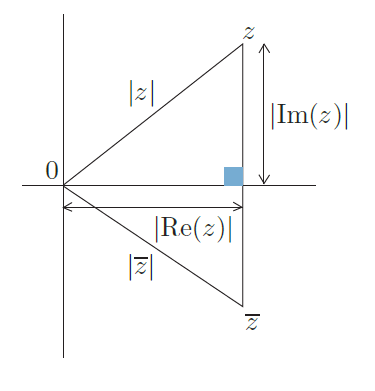
\includegraphics[width=0.3\textwidth]{./figs/fig-s-0-1}
\end{center}
%\caption{$RP$와 $SQ$는 길이가 같고 수직으로 만난다}
%\label{fig-5-5}
\end{figure*}

\subsection*{연습문제 \ref{ex-1-17}}

우선 $|\bar az| = |\bar a||z| = |a||z| <1\cdot 1 =1$이므로, $\bar az \ne 1$이고,
\begin{align*}
\dfrac{z-a}{1-\bar az}\cdot \overline{\left(\dfrac{z-a}{1-\bar az}\right)}
&= \dfrac{z-a}{1-\bar az}\cdot \dfrac{\bar z-\bar a}{1-a\bar z}
= \dfrac{z\bar z - a\bar z - \bar a z+a\bar a}{1-a\bar z - \bar a z + a\bar a z \bar z} \\
&= \dfrac{|z|^2 - a\bar z - \bar a z + |a|^2}{1-a\bar z - \bar a z + |a|^2|z|^2} \\
&= \dfrac{1 - a\bar z - \bar a z + |a|^2|z|^2+|z|^2+|a|^2-1-|a|^2|z|^2}
{1-a\bar z - \bar a z + |a|^2|z|^2} \\
&= 1 + \dfrac{|z|^2+|a|^2-1-|a|^2|z|^2}{1-a\bar z - \bar a z + |a|^2|z|^2} \\
&= 1 + \dfrac{|z|^2+|a|^2-1-|a|^2|z|^2}{|1- \bar a z|^2} \\
&= 1 -  \dfrac{(1-|z|^2)(1-|a|^2)}{|1- \bar a z|^2}.
\end{align*}
따라서
$\left| \dfrac{z-a}{1-\bar az} \right|^2 = 1 -
\underbrace{\dfrac{(1-|z|^2)(1-|a|^2)}{|1- \bar a z|^2}}_{\ge0\ (|z|<1, |a|<1\text{ 이므로})}
\le 1-0 = 1$.

\subsection*{연습문제 \ref{ex-1-18}}

$w\in\mathbb C$가 $p(w)=0$, 즉,
$c_0 + c_1w + \cdots + c_dw^d=0$을 만족한다고 하자. 
그러면,
\[
\overline{c_0 + c_1w + \cdots + c_dw^d} = \bar 0 = 0
\]
이고, 모든 $c_k$ ($0\le k\le d$)가 실수이므로
\begin{align*}
0 & = \overline{c_0 + c_1w + \cdots + c_dw^d} 
= \overline{c_0} + \overline{c_1w} + \cdots + \overline{c_dw^d} \\
&= \overline{c_0} + \overline{c_1}\overline{w} + \cdots + \overline{c_d}\overline{w^d}
= c_0 + c_1\overline{w} + \cdots + c_d(\bar w)^d.
\end{align*}
마지막 등식에서 
\[
\overline{w^k} = \underbrace{\overline{w\cdots w}}_{k\text{번}}
= \underbrace{\bar w \cdots \bar w}_{k\text{번}}
= (\bar w)^k,
\quad 1\le k \le d
\]
를 사용하였다.
따라서, $0=c_0 + c_1\overline{w} + \cdots + c_d(\bar w)^d = p(\bar w)$.

\subsection*{연습문제 \ref{ex-1-19}}

$a = |a|(\cos\alpha + i\sin\alpha)$, 
$b = |b|(\cos\beta + i\sin \beta)$라고 하자.
단, $\alpha, \beta \in [0,2\pi)$. 그러면,
\begin{align*}
a\bar b &= |a|(\cos\alpha + i\sin\alpha)\cdot
|b|(\cos\beta - i\sin \beta) \\
&=|a||b|(\cos\alpha + i\sin\alpha)(\cos\beta - i\sin \beta)
\end{align*}
이고 $\Im(a\bar b) = |a||b|(-(\cos\alpha)(\sin\beta) + (\sin\alpha)(\cos\beta))
= |a||b|\sin(\alpha-\beta)$.
$0$, $a$, $b$를 꼭지점으로 하는 $\Delta OAB$의 면적은
($O\equiv 0$, $A\equiv a$, $B\equiv b$)
\[
\dfrac12 \ell(OA)\ell(OB) \cdot \sin \angle AOB
= \dfrac12 |a|\cdot |b| \cdot |\sin(\alpha-\beta)|
= \dfrac12 |\Im(a\bar b)| = \left| \dfrac{\Im(a\bar b)}2\right|.
\]

\begin{figure}[h!]
\begin{center}
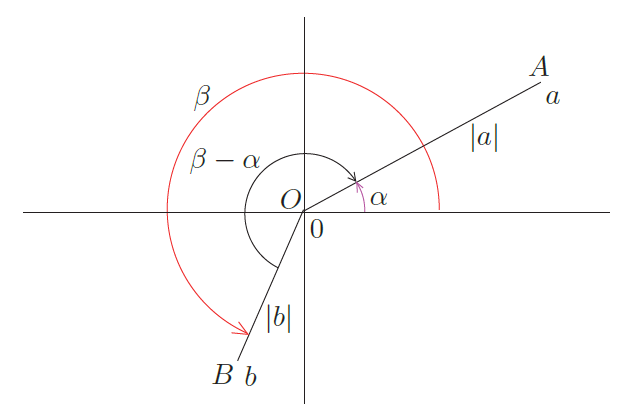
\includegraphics[width=0.7\textwidth]{./figs/fig-5-6}
\end{center}
\caption{$0$, $a$, $b$를 꼭지점으로 하는 $\Delta OAB$의 면적}
\label{fig-5-6}
\end{figure}

\subsection*{연습문제 \ref{ex-1-20}}

$z_1, z_2, z_3 \in\mathbb C$에 대하여,
\[
w:= \overline{i\cdot \det \begin{bmatrix}
1 & z_1 & \overline{z_1} \\
1 & z_2 & \overline{z_2} \\
1 & z_3 & \overline{z_3}
\end{bmatrix}}
= -i\cdot \overline{\det \begin{bmatrix}
1 & z_1 & \overline{z_1} \\
1 & z_2 & \overline{z_2} \\
1 & z_3 & \overline{z_3}
\end{bmatrix}}.
\]
한편, 정사각행렬 $M=[m_{ij}]$에 대하여,
\[
\det M = \sum_{\sigma\in S_n} (\sgn \sigma) \cdot m_{i\sigma(i)},
\]
여기서, $S_n$은 $\{1,\ldots, n\}$에 대한 모든 치환(permutation)의 집합이다.
\[
\overline{\det M} = \sum_{\sigma\in S_n} (\sgn \sigma) \cdot
\overline{m_{i\sigma(i)}} = \det \overline{M},
\]
여기서, $\overline{M}$은 $M$의 모든 원소에 대하여 켤레복소수를 취한 것이다.
따라서,
\[
\overline{\det \begin{bmatrix}
1 & z_1 & \overline{z_1} \\
1 & z_2 & \overline{z_2} \\
1 & z_3 & \overline{z_3}
\end{bmatrix}}
= \det \begin{bmatrix}
1 & \overline{z_1} & z_1 \\
1 & \overline{z_2} & z_2 \\
1 & \overline{z_3} & z_3
\end{bmatrix}
= -  \det \begin{bmatrix}
1 & z_1 & \overline{z_1} \\
1 & z_2 & \overline{z_2} \\
1 & z_3 & \overline{z_3}
\end{bmatrix},
\]
마지막 등식은 두번째 열과 세번째 열을 바꾼 것이다.
종합하면,
\begin{align*}
\overline{i\cdot \det \begin{bmatrix}
1 & z_1 & \overline{z_1} \\
1 & z_2 & \overline{z_2} \\
1 & z_3 & \overline{z_3}
\end{bmatrix}}
= -i\cdot \overline{\det \begin{bmatrix}
1 & z_1 & \overline{z_1} \\
1 & z_2 & \overline{z_2} \\
1 & z_3 & \overline{z_3}
\end{bmatrix}}
& = -i \cdot \left(
-  \det \begin{bmatrix}
1 & z_1 & \overline{z_1} \\
1 & z_2 & \overline{z_2} \\
1 & z_3 & \overline{z_3}
\end{bmatrix}
\right) \\
& = i \cdot  \det \begin{bmatrix}
1 & z_1 & \overline{z_1} \\
1 & z_2 & \overline{z_2} \\
1 & z_3 & \overline{z_3}
\end{bmatrix}.
\end{align*}
따라서, $w$는 켤레복소수와 동일하므로 실수이다.

\subsection*{연습문제 \ref{ex-1-21}}

\begin{align*}
|z_1+z_2|^2 + & |z_1 - z_2|^2 \\
&= (z_1 + z_2)(\overline{z_1} + \overline{z_2}) + (z_1 - z_2)(\overline{z_1} - \overline{z_2}) \\
&= z_1\cdot \overline{z_1} + z_1 \cdot \overline{z_2} + z_2 \cdot \overline{z_1}
+ z_2\cdot \overline{z_2} \\
&\qquad + z_1\overline{z_1} + z_1\cdot(-\overline{z_2}) + (-z_2)\cdot\overline{z_1}
+ (-z_2)(-\overline{z_2}) \\
& = |z_1|^2 + \cancel{z_1 \cdot \overline{z_2}} + \cancel{z_2 \cdot \overline{z_1}}
+ |z_2|^2 + |z_1|^2 - \cancel{z_1 \cdot \overline{z_2}}  
- \cancel{z_2 \cdot \overline{z_1}} + |z_2|^2 \\
&= 2(|z_1|^2 + |z_2|^2).
\end{align*}

복소평면에서 $0$, $z_1$, $z_2$, $z_1+z_2$를 꼭지점으로 하는 평행사변형 $P$를 생각하자.
그러면, $|z_1+z_2|$는 $P$의 한쪽 대각선의 길이가 되고,
$|z_1-z_2|$는 다른쪽 대각선의 길이가 된다. 또한, $|z_1|$, $|z_2|$는
$P$의 두변의 길이다. 따라서 위의 식이 의미하는 것은
``평행사변형에서 대각선 길이의 제곱의 합은 변의 길이의 제곱의 합의 두배와 같다'' 이다.

\subsection*{연습문제 \ref{ex-1-22}}

$z_1, z_2\in\mathbb C$에 대하여,
$|z_1| = |z_1 - z_2 + z_2| \le |z_1 - z_2| + |z_2|$이므로
\begin{equation} \label{eq-5-12}
|z_1| - |z_2| \le |z_1 - z_2|.
\end{equation}
모든 $z_1, z_2\in\mathbb C$에 대하여,
식 \eqref{eq-5-12}에서 $z_1$과 $z_2$의 역할을 바꾸어도 성립하므로
\begin{equation}\label{eq-5-13}
|z_2| - |z_1| \le |z_2 - z_1| = |-(z_1-z_2)|
= |-1| |z_1-z_2| =|z_1-z_2|.
\end{equation}
식 \ref{eq-5-12}\와 \ref{eq-5-13}\로부터 
$\left| |z_1| -|z_2| \right| \le |z_1 - z_2|$이다.

\subsection*{연습문제 \ref{ex-1-23}}

\begin{itemize}
\item[(1),(2),(3):] \
\begin{figure}[h!]
\begin{center}
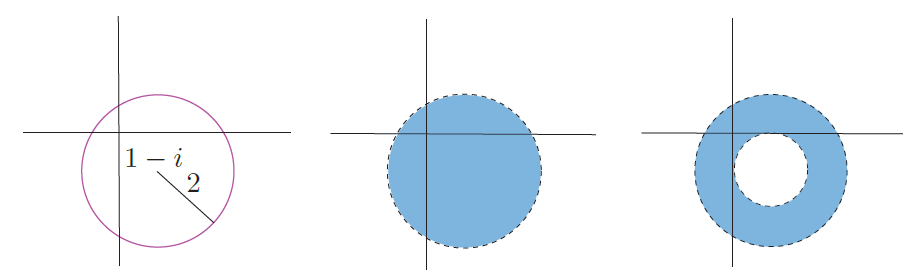
\includegraphics[width=0.8\textwidth]{./figs/fig-5-7}
\end{center}
\caption{왼쪽부터 $|z-(1-i)|=2$, $|z-(1-i)|<2$,
$1<|z-(1-i)|<2$}
\label{fig-5-7}
\end{figure}
\item[(4):] $z=x+iy$ ($x,y\in\mathbb R$)이라 하면,
$\Re(z-(1-i))=3$은 $x-1=3$과 동치이므로, $x=4$이다.
\begin{figure*}[h!]
\begin{center}
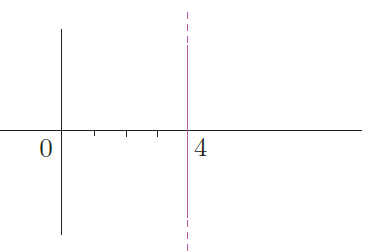
\includegraphics[width=0.3\textwidth]{./figs/fig-s-0-2}
\end{center}
%\caption{$RP$와 $SQ$는 길이가 같고 수직으로 만난다}
%\label{fig-5-5}
\end{figure*}
\item[(5):] $z=x+iy$ ($x,y\in\mathbb R$)이라 하면,
$|\Im(z-(1-i))|<3$은 $|y+1|<3$, 즉, $-4<y<2$와 같다.
\begin{figure*}[h!]
\begin{center}
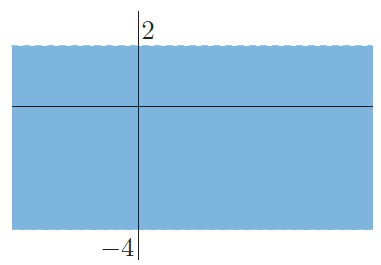
\includegraphics[width=0.3\textwidth]{./figs/fig-s-0-3}
\end{center}
%\caption{$RP$와 $SQ$는 길이가 같고 수직으로 만난다}
%\label{fig-5-5}
\end{figure*}
\item[(6):] $\{ z\in\mathbb C\,:\, |z-(1-i)| = |z-(1+i)|\}$는
$1-i$와 $1+i$에서 같은 거리에 있는 복소수 $z$의 집합이다.
따라서, $1-i$와 $1+i$을 잇는 선분의 수직이등분선이 된다.
즉, 실수축이다.
\begin{figure}[h!]
\begin{center}
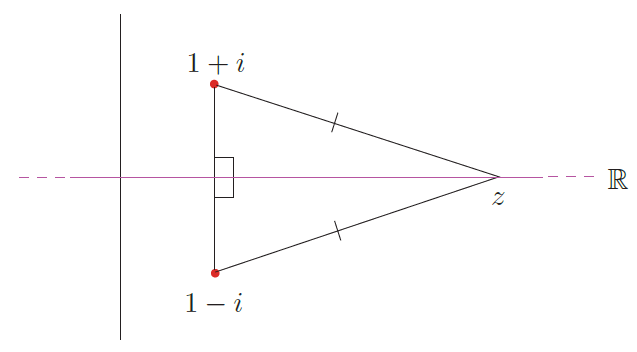
\includegraphics[width=0.6\textwidth]{./figs/fig-5-8}
\end{center}
\caption{$|z-(1-i)| = |z-(1+i)|$를 만족하는 집합은 $\mathbb R$}
\label{fig-5-8}
\end{figure}
\item[(7):] 방정식 $|z-(1-i)| + |z-(1+i)| =2$는 
$z$에서 $1+i$까지의  거리와  $1-i$까지의 거리의 합이 $2$가 됨을 의미한다.
그런데 $1-i$와 $1+i$의 거리가 $2$이므로
$z$는 $1-i$와 $1+i$를 잇는 선분에 있다.

직접 계산하는 방식으로도 같은 결과를 얻을 수 있다.
$z=x+iy$ ($x,y\in\mathbb R$)이면
\begin{align*}
2 &= \sqrt{(x-1)^2 + (y+1)^2} + \sqrt{(x-1)^2 + (y-1)^2} \\
&\ge |y+1| + |y-1| \ge 1 + \cancel{y} + 1 - \cancel{y} =2
\end{align*}
이므로 $|y+1| + |y-1|=2$이고, $x=1$이다.
\begin{figure}[h!]
\begin{center}
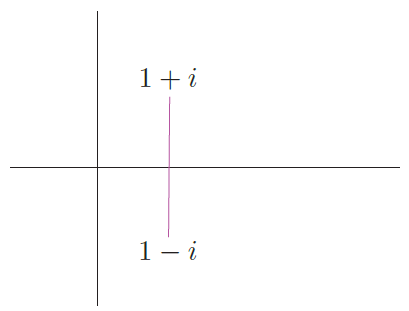
\includegraphics[width=0.6\textwidth]{./figs/fig-5-9}
\end{center}
\caption{$|z-(1-i)| + |z-(1+i)|=2$를 만족하는 집합은 $1-i$와 $1+i$를 잇는 선분이다.}
\label{fig-5-9}
\end{figure}
\item[(8):] 방정식 $|z-(1-i)| + |z-(1+i)| =3$을 만족하는 집합은
초점이 $1+i$와 $1-i$인 타원 $E$이 된다.
따라서, $\{z\in\mathbb C\,:\, |z-(1-i)| + |z-(1+i)| < 3\}$은
타원 $E$의 내부가 된다.
\begin{figure}[h!]
\begin{center}
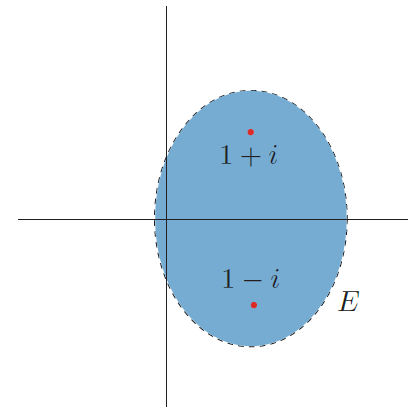
\includegraphics[width=0.6\textwidth]{./figs/fig-5-10}
\end{center}
\caption{$|z-(1-i)| + |z-(1+i)| < 3$을 만족하는 집합은 타원  $E$의 내부이다.}
\label{fig-5-10}
\end{figure}
\end{itemize}

\subsection*{연습문제 \ref{ex-1-24}}

$z\ne0$에 대하여
$p(z) = z^d \left( c_d + \dfrac{c_{d-1}}z + \cdots + \dfrac{c_1}{z^{d-1}}
+ \dfrac{c_0}{z^d} \right)$.
\[
\lim_{n\to\infty}  \left( 
 \dfrac{|c_{d-1}|}n + \cdots + \dfrac{|c_1|}{n^{d-1}}
+ \dfrac{|c_0|}{n^d} \right) = 0
\]
이므로, 
다음을  만족하도록 충분히 큰 $N$을 잡을 수 있다.
\[
\dfrac{|c_{d-1}|}N + \cdots + \dfrac{|c_1|}{N^{d-1}}
+ \dfrac{|c_0|}{N^d} < \dfrac{|c_d|}2.
\]
그러면 $|z|>N=:R$에 대하여
\begin{align*}
|p(z)| &= |z^d| \left|
c_d + \dfrac{c_{d-1}}z + \cdots + \dfrac{c_1}{z^{d-1}}
+ \dfrac{c_0}{z^d} \right| \\
&\ge |z|^d \left( |c_d| - \left| \dfrac{c_{d-1}}z + \cdots + \dfrac{c_1}{z^{d-1}}
+ \dfrac{c_0}{z^d} \right| \right) \\
&\ge |z|^d \left(|c_d| - \left( \dfrac{|c_{d-1}|}{|z|} + \cdots + \dfrac{|c_1|}{|z|^{d-1}}
+ \dfrac{|c_0|}{|z|^d} \right) \right) \\
&\ge |z|^d \left(|c_d| - \left( \dfrac{|c_{d-1}|}N + \cdots + \dfrac{|c_1|}{N^{d-1}}
+ \dfrac{|c_0|}{N^d} \right) \right) \\
&\ge |z|^d \left(|c_d| - \dfrac{|c_d|}2 \right) = \underbrace{\dfrac{|c_d|}2}_{=:M} |z|^d.
\end{align*}

\subsection*{연습문제 \ref{ex-1-25}}

$(\Leftarrow):$ 

실수열 $(\Re(z_n))_{n\in\mathbb N}$과 
$(\Im(z_n))_{n\in\mathbb N}$가 각각 $\Re(L)$과 $\Im(L)$로 수렴한다고 하자.
그러면, 주어진 $\epsilon>0$에 대하여,
충분히 큰 $N$이 존재하여 $n>N$이면
\[
|\Re(z_n) - \Re(L)| < \dfrac\epsilon{\sqrt{2}},\quad
|\Im(z_n) - \Im(L)| < \dfrac\epsilon{\sqrt{2}}
\]
을 만족하게 할 수 있고,
\begin{align*}
|z_n-L| &= \sqrt{ (\Re(z_n) - \Re(L))^2 + (\Im(z_n) - \Im(L))^2} \\
&< \sqrt{\left(\dfrac\epsilon{\sqrt{2}}\right)^2  + \left(\dfrac\epsilon{\sqrt{2}}\right)^2}
= \epsilon.
\end{align*}
따라서 $(z_n)_{n\in\mathbb N}$은 $L$로 수렴한다.

\noindent $(\Rightarrow):$

$(z_n)_{n\in\mathbb N}$이 $L$로 수렴한다고 가정하자.
$n>N$이면  $|z-L|<\epsilon$이 되도록 하는 $N$을 잡을 수 있다.
그러면 모든 $n>N$에 대하여,
\begin{align*}
|\Re(z_n) - \Re(L)| &= |\Re(z_n -L)| \le |z_n -L| <\epsilon, \\
|\Im(z_n) - \Re(L)| &= |\Im(z_n -L)| \le |z_n -L| <\epsilon
\end{align*}
이 되어
$(\Re(z_n))_{n\in\mathbb N}$과 
$(\Im(z_n))_{n\in\mathbb N}$이 각각 
$\Re(L)$과 $\Im(L)$로 수렴한다.

\subsection*{연습문제 \ref{ex-1-26}}

$(\Rightarrow):$

$(z_n)_{n\in\mathbb N}$이 $L$로 수렴한다고 가정하자.
그러면 $(\Re(z_n))_{n\in\mathbb N}$과 
$(\Im(z_n))_{n\in\mathbb N}$이 각각 
$\Re(L)$과 $\Im(L)$로 수렴한다.
따라서 $(\Re(z_n))_{n\in\mathbb N}$과 
$(-\Im(z_n))_{n\in\mathbb N}$은 각각 
$\Re(L)$과 $-\Im(L)$로 수렴한다.
즉, $(\Re(\overline{z_n}))_{n\in\mathbb N}$과 
$(\Im(\overline{z_n}))_{n\in\mathbb N}$이 각각 
$\Re(\overline{L})$과 $\Im(\overline{L})$로 수렴한다.
결론적으로 $(\overline{z_n})_{n\in\mathbb N}$이 $\overline{L}$로 수렴한다.

\noindent $(\Leftarrow):$ 

$(\overline{z_n})_{n\in\mathbb N}$이 $\overline{L}$로 수렴한다고 하자.
앞의 증명에서 $(\overline{(\overline{z_n})})_{n\in\mathbb N}$이 
$\overline{(\overline{L})}$로 수렴한다.
다시 쓰면, $(z_n)_{n\in\mathbb N}$이 $L$로 수렴한다.

\subsection*{연습문제 \ref{ex-1-27}}




%===[salt] 2장
% !TEX root = ./CA_solution.tex

\section*{2장 - 연습문제 풀이}

\subsection*{연습문제 \ref{ex-2-1}}

$z\ne0$에 대하여
\[
\dfrac{f(z) - f(0)}{z-0} - 0 = \dfrac{|z|^2-0}{z-0} = \dfrac{|z|^2}z.
\]
주어진 $\epsilon>0$에 대하여 $ \delta=\epsilon$으로 잡으면,
$0<|z-0|=|z| <\delta$일 때,
\[
\left| \dfrac{f(z) - f(0)}{z-0} - 0\right|
= \left| \dfrac{|z|^2}z \right|  = \dfrac{|z|^2}{|z|} = |z| < \delta = \epsilon.
\]
따라서 $f$는 $0$에서 복소미분가능하고 $f'(0)=0$이다.

\subsection*{연습문제 \ref{ex-2-2}}

$w_0\in \mathbb D^*$라 하자. 그러면 $\overline{w_0}\in D$이다.
$f$가 $D$에서 복소해석함수이므로, 주어진 $\epsilon>0$에 대응하는 
$\delta>0$가 존재하여,
$0<|z-\overline{w_0}| < \delta$이면 $z\in D$와
\begin{equation}\label{eq-5-17}
\left| \dfrac{f(z) - f(\overline{w_0})}{z-\overline{w_0}} - f'(\overline{w_0}) \right| < \epsilon
\end{equation}
를 만족한다.
이제 $w$를 $0<|w-w_0| <\delta$로 잡으면
\[
0< |w-w_0| = |\overline{w-w_0}| = |\overline{w} - \overline{w_0}| < \delta
\]
이 되어 $w\in D^*$이다.
또한,
\begin{align*}
\left| \dfrac{f^*(w) - f^*(w_0)}{w-w_0} - \overline{f'(\overline{w_0})} \right|
&= \left| \dfrac{\overline{f(\overline{w})} - \overline{f(\overline{w_0})}}{w-w_0} 
- \overline{f'(\overline{w_0})} \right| \\
&= \left| \overline{ \dfrac{f(\overline{w}) - f(\overline{w_0})}{w-w_0} 
- f'(\overline{w_0})} \right| \\
&= \left| \dfrac{f(\overline{w}) - f(\overline{w_0})}{w-w_0} 
- f'(\overline{w_0}) \right| < \epsilon \text{ \ (식 \eqref{eq-5-17}\을 이용하여)}
\end{align*}
이 되므로, $f^*$는 $w_0$에서 복소미분가능하며
$(f^*)'(w_0)= \overline{f'(\overline{w_0})}$이다.
$w_0\in D^*$를 임의로 선택할 수 있으므로
$f^*$는 $D^*$에서 복소미분가능함수이다.

\subsection*{연습문제 \ref{ex-2-3}}

$f$가 $z_0$에서 복소미분가능하므로,
상수 $r>0$과 함수 $h:D(z_0,r)\to \mathbb C$가 존재하여
$|z-z_0|<r$에 대하여
\[
f(z) = f(z_0) + (f'(z_0) + h(z))(z-z_0)
\]
로 쓸 수 있고
\[
\lim_{z\to z_0} h(z) = 0
\]
이다.
여기서, $D(z_0,r):= \{ z\in \mathbb C \,:\, |z-z_0| < r\} \subset D$이다.

$D(z_0,r'):= \{ z\in \mathbb C \,:\, |z-z_0| < r'\} \subset D(z_0,r) \subset D$과
$|h(z)|<1$이 되도록 $r'<r$을 잡자.
이제 주어진 $\epsilon>0$에 대하여
\[
\delta = \min\left\{ \dfrac\epsilon{|f'(z_0)|+1}, r' \right\}
\]
로 선택하면, $0<|z-z_0|<\delta$일 때, 
$z\in D(z_0, r')$이고,
\begin{align*}
|f(z) - f(z_0)| = |f'(z_0) + h(z)||z-z_0|
&\le ( |f'(z_0)|+|h(z)|)\dfrac{\epsilon}{ |f'(z_0)|+1} \\
&< ( |f'(z_0)|+1)  \dfrac{\epsilon}{|f'(z_0)|+1} = \epsilon.
\end{align*}
따라서 $f$는 $z_0$에서 연속이다.

\subsection*{연습문제 \ref{ex-2-4}}

$f,g:U\to \mathbb C$가 $z_0\in U$에서 복소미분가능함을 이용하면,
보조정리 \ref{lem-2-1}\로부터
$r>0$과 $h_f, h_g: D(z_0,r) \to \mathbb C$가 존재하여
(단, $D(z_0,r):= \{ z\in \mathbb C \,:\, |z-z_0| < r\}$)

$|z-z_0|<r$이면,
\begin{align}
f(z) & = f(z_0) + (f'(z_0) +h_f(z))(z-z_0), \label{eq-5-18} \\
g(z) & = g(z_0) + (g'(z_0) +h_g(z))(z-z_0), \label{eq-5-19}
\end{align}
와 $\Lim_{z\to z_0} h_f(z)  = 0 = \Lim_{z\to z_0} h_g(z)$를 만족한다.
\begin{itemize}
\item[(1)] 식 \eqref{eq-5-18}\과 \eqref{eq-5-19}\를 더하면,
$|z-z_0|<r$에 대하여
\[
(f+g)(z) = (f+g)(z_0) + \left( f'(z_0) + g'(z_0) + h_{f+g}(z) \right)(z-z_0)
\]
를 만족한다. 단, $D(z_0,r)$에서 $h_{f+g} (z) := h_f(z) + h_g(z)$로 정의한다.
또한,
\[
\lim_{z\to z_0} h_{f+g}(z) = \lim_{z\to z_0} ( h_f(z) + h_g(z) )
= \lim_{z\to z_0} h_f(z) + \lim_{z\to z_0} h_g(z) = 0+0 = 0.
\]
보조정리 \ref{lem-2-1}에 의하여
$f+g$는 복소미분가능하며 $(f+g)'(z_0) = f'(z_0) + g'(z_0)$이다.
\item[(2)] 식 \eqref{eq-5-18}에 $\alpha$를 곱하면,
$|z-z_0|<r$에 대하여
\[
(\alpha \cdot f)(z) = (\alpha \cdot f)(z_0) + \left(
\alpha\cdot f'(z_0) + h_{\alpha\cdot f}(z) \right) (z-z_0),
\]
단, $D(z_0,r)$에서 $h_{\alpha\cdot f}(z) := \alpha \cdot f(z)$이다.
또한,
\[
\lim_{z\to z_0} h_{\alpha\cdot f}(z) = \lim_{z\to z_0} (\alpha\cdot h_f(z))
= \alpha \cdot \lim_{z\to z_0} h_f(z) = \alpha\cdot 0 = 0.
\]
보조정리 \ref{lem-2-1}에 의하여
$\alpha \cdot f$는 복소미분가능하며 $(\alpha\cdot f)'(z_0) =\alpha\cdot f'(z_0)$이다.

\item[(3)] 식 \eqref{eq-5-18}\과 \eqref{eq-5-19}\를 곱하면,
$|z-z_0|<r$에 대하여
\[
(fg)(z) = (fg)(z_0) + \left( f'(z_0)g(z_0) + f(z_0)g'(z_0) + h_{fg}(z) \right) (z-z_0),
\]
단, $D(z_0,r)$에서
\[
h_{fg}(z):= f(z_0)h_g(z) + g(z_0)h_f(z) + (z-z_0)(f'(z_0)+h_f(z))(g'(z_0)+h_g(z))
\]
또한,
\[
\lim_{z\to z_0} h_{fg}(z) = f(z_0)\cdot0 + g(z_0)\cdot 0 
+ 0\cdot (f'(z_0)+0)\cdot(g'(z_0)+0)=0
\]
이므로 $fg$는 $z_0$에서 복소미분가능하며
\[
(fg)'(z) = f'(z_0)g(z_0) + f(z_0)g'(z_0).
\]
\end{itemize}

\subsection*{연습문제 \ref{ex-2-5}}

$\Hol(\mathbb D)$가 $d$차의 유한차원이라고 하자.
그러면 $d+1$개의 벡터 $1,z, z^2, \ldots, z^d\in \Hol(\mathbb  D)$는
일차종속이다. 따라서 모두 $0$은 아닌 $\alpha_0, \ldots, \alpha_d$가 존재하여
\[
\alpha_0\cdot 1 + \alpha_1\cdot z + \cdots + \alpha_d \cdot z^d = 0
\quad(z\in \mathbb D)
\]
을 만족한다.
$k\in \{0, 1, \ldots, d\}$를 $\alpha_k \ne 0$인 가장 작은 값이라 하자.
그러면, $k$번 미분한 값을 $0\in \mathbb D$에서 계산하면
\[
0 + \alpha_k \cdot k! + 0 = 0
\]
이므로 $\alpha_k=0$이 되어 모순이다.

\subsection*{연습문제 \ref{ex-2-6}}

$z_0\in U$라 하자. $f$는 $z_0$에서 복소미분가능하므로
$r>0$과 $D(z_0,r) := \{ z\in \mathbb C\,:\, |z-z_0|<r\} \subset U$에 정의된
복소함수 $h$가 존재하여
\[
f(z) = f(z_0) + (f'(z_0) +h(z))(z-z_0),
\quad z\in D(z_0,r)
\]
과
\begin{equation}\label{eq-5-20}
\lim_{z\to z_0} h(z)=0
\end{equation}
을 만족한다.
$g:=1/f$라 하면,
\[
\dfrac1{g(z)} = \dfrac1{g(z_0)} + (f'(z_0) +h(z))(z-z_0)
\]
이므로 $g(z_0) = g(z) + (f'(z_0)+h(z))g(z_0)g(z)\cdot(z-z_0)$.
정리하면
\begin{align*}
g(z) &= g(z_0) + (-f'(z_0)g(z_0)g(z) - h(z)g(z_0)g(z)))\cdot(z-z_0) \\
&= g(z_0) + \left( - \dfrac{f'(z_0)}{(f(z_0))^2} + \dfrac{f'(z_0)}{(f(z_0))^2}
- \dfrac{f'(z_0)}{f(z_0)f(z)} - \dfrac{h(z)}{f(z_0)f(z)} \right) (z-z_0) \\
&= g(z_0) + \left( - \dfrac{f'(z_0)}{(f(z_0))^2} + \varphi(z) \right)\cdot(z-z_0),
\end{align*}
$z\in D(z_0,r)$에서
\[
\varphi(z):= \dfrac{f'(z_0)}{(f(z_0))^2}
- \dfrac{f'(z_0)}{f(z_0)f(z)} - \dfrac{h(z)}{f(z_0)f(z)}.
\]
$z_0$에서 $f$의 연속성과 식 \eqref{eq-5-20}\로부터
\[
\lim_{z\to z_0} \varphi(z) = \cancel{\dfrac{f'(z_0)}{(f(z_0))^2}}
- \cancel{\dfrac{f'(z_0)}{f(z_0)f(z_0)}} - \dfrac{0}{f(z_0)f(z_0)} = 0.
\]
따라서 $g$가 $z_0$에서 복소미분가능하며
\[
g'(z_0) = - \dfrac{f'(z_0)}{(f(z_0))^2}.
\]

\subsection*{연습문제 \ref{ex-2-7}}

$m\ge0$인 경우는 이미 증명했으므로, 
$m= -n$ ($n\in \mathbb N$)인 경우를 생각하자.
$f(z):=z^n$ ($z\in \mathbb C\setminus \{0\}$)에  대하여 함수
\[
z\mapsto z^m = z^{-n} = \dfrac1{z^n} = \dfrac1{f(z)}
\]
는 복소해석함수이고 $\mathbb C\setminus \{0\}$에서 함수값이
$0$은 아니므로
$1/f$도 복소해석함수이고, 미분은
\[
\left(\dfrac1f\right)'(z) = - \dfrac{f'(z)}{(f(z))^2} = - \dfrac{nz^{n-1}}{(z^n)^2}
= -n \dfrac1{z^{n+1}} = m \cdot \dfrac1{z^{-m+1}} = mz^{m-1}
\]
이 되어 증명이 끝난다.

\subsection*{연습문제 \ref{ex-2-8}}

$f: \mathbb D \to \mathbb C$를 
\[
f(z) = -\dfrac{1+z}{1-z},\quad z\in \mathbb D
\]
로 정의하고, $f: \mathbb C \to \mathbb C$를 $g(z)= \exp z$로 정의하자.
그러면, $f(\mathbb D) \subset \mathbb C = D_g$.
따라서 $g\circ f$는 $\mathbb D$에서 복소해석함수이고,
\begin{align*}
(g\circ g)'(z) &= g'(f(z))\cdot f'(z) 
= \exp\left( - \dfrac{1+z}{1-z}\right) \cdot \dfrac d{dz}\left( - \dfrac{1+z}{1-z}\right) \\
&= \exp\left( - \dfrac{1+z}{1-z}\right)\cdot \left(
-(1+z)\dfrac d{dz} \left(\dfrac1{1-z}\right) - \dfrac1{1-z}\dfrac d {dz}(1+z)\right) \\
&= \exp\left( - \dfrac{1+z}{1-z}\right) \cdot \left(
-\dfrac{1+z}{(1-z)^2} - \dfrac1{1-z} \right) \\
&= - \dfrac2{(1-z)^2} \exp\left( - \dfrac{1+z}{1-z}\right).
\end{align*}
따라서, $z\in\mathbb D$에 대하여,
$\dfrac d{dz} \left( \exp\left( - \dfrac{1+z}{1-z}\right) \right)
=  - \dfrac2{(1-z)^2} \exp\left( - \dfrac{1+z}{1-z}\right)$.

\subsection*{연습문제 \ref{ex-2-9}}

$z = x+iy$ ($x,y\in\mathbb R$)라 하면,
$|z|^2 = x^2+y^2$.
따라서, $u, v$를 각각 $|z|^2$의 실수부와 허수부라 하면,
$u=x^2+y^2$, $v=0$이다. 따라서,
\begin{align*}
\dfrac{\partial u}{\partial x} &=2x, \quad \dfrac{\partial v}{\partial y} = 0, \\
\dfrac{\partial u}{\partial y} &=2y, \quad \dfrac{\partial v}{\partial x} = 0.
\end{align*}
$z\ne0$이므로, $x$ 또는 $y$중 하나는 $0$이 아니다.
즉, 코시-리만 방정식 중 적어도 하나는 만족되지 않는다.
\begin{align*}
\left( \dfrac{\partial u}{\partial x} = \right) 2x &\ne 0 
\left( = \dfrac{\partial v}{\partial y} \right) \text{ 또는} \\
\left( \dfrac{\partial u}{\partial y} = \right) 2y &\ne 0 
\left( = - \dfrac{\partial v}{\partial x} \right).
\end{align*}
결론적으로 $|z|^2$은 $0$이 아닌 점에서 미분이 불가능하다.

\subsection*{연습문제 \ref{ex-2-10}}

$z = x+iy$ ($x,y\in\mathbb R$)라 하면,
\begin{align*}
z^3 &= (x+iy)^3 = x^3 + 3x^2(iy) + 3x(iy)^2 + (iy)^3 \\
&= x^3 - 3xy^2 + i(3x^2y-y^3).
\end{align*}

$u$, $v$를 각각 $z^3$의 실수부와 허수부라 하면,
\begin{align*}
u(x,y) &= x^3 -3xy^2, \\
v(x,y) &= 3x^2y - y^3.
\end{align*}

$u$, $v$는 연속미분가능하고 (즉, $u,v\in C^1$)
\begin{align*}
\dfrac{\partial u}{\partial x} &= 3x^2 -2y^2 = \dfrac{\partial v}{\partial y} \text{ 이고}, \\
\dfrac{\partial u}{\partial y} &= -6xy = - \dfrac{\partial v}{\partial x}.
\end{align*}
즉, $\mathbb R^2$의 모든 점에서 코시-리만 방정식을 만족하므로,
$z\mapsto z^3$은 전해석함수이다.

\subsection*{연습문제 \ref{ex-2-11}}

$z = x+iy$ ($x,y\in\mathbb R$)라 하면,
$\Re(z) = \Re(x+iy) = x$.
따라서, $u, v$를 각각 $\Re(z)$의 실수부와 허수부라 하면,
\begin{align*}
u & =x, \\
v &=0.
\end{align*}
따라서, 모든 $(x,y) \in \mathbb R^2$에서
\[
\dfrac{\partial u}{\partial x}  = 1 \ne 0 =  \dfrac{\partial v}{\partial y}.
\]
즉, 코시-리만 방정식은 $\mathbb R^2$의 어떤 점에서도 만족되지 않는다.
결론적으로 $\mathbb C$의 모든 점에서 $\Re(z)$는 복소미분가능하지 않다.

\subsection*{연습문제 \ref{ex-2-12}}

$u$, $v$를 각각 $f$의 실수부와 허수부라 하자. 
그러면, $v=0$이고,
\[
\dfrac{\partial u}{\partial x} = \dfrac{\partial v}{\partial y} = 0
\text{ 이고 }
\dfrac{\partial u}{\partial y} = - \dfrac{\partial v}{\partial x} = 0.
\]
따라서 
\[
u(x,y_0) = u(x_0,y_0) = \int_{x_0}^z \dfrac{\partial u}{\partial y}(\xi, y_0) d\xi = 0
\]







%




%===[salt] 3장
% !TEX root = ../CA_book.tex

\section*{3장 - 연습문제 풀이}

\subsection*{연습문제 \ref{ex-3-1}}

$\gamma_1 = \cos t + i\sin t$, $\gamma_2 = \cos (2t) + i\sin (2t)$,
$\gamma_3 = \cos t - i\sin t$이므로
$k=1,2,3$ 각각의 경우 모두 $(\Re(\gamma_k(t)))^2 + (\Im(\gamma_k(t)))^2=1$이다.
$\gamma_k$의 상은 중심이 $0$이고 반지름이 $1$인 원 $\mathbb T$에 있다.
$\theta \in [0,2\pi)$에 대하여 $z = \exp(i\theta)$이면,
$z = \gamma_1(\theta) = \gamma_2(\theta/2) = \gamma_3(2\pi - \theta)$이다.
따라서 $\mathbb T$위의 모든 점은 $\gamma_1, \gamma_2, \gamma_3$ 각각에 의한 상에
속한다.
\begin{align*}
\int_{\gamma_1} \dfrac1z dz &= \int_0^{2\pi} \dfrac1{\exp(it)}\cdot i\exp(it)dt = 2\pi i, \\
\int_{\gamma_2} \dfrac1z dz &= \int_0^{2\pi} \dfrac1{\exp(2it)}\cdot 2i\exp(2it)dt = 4\pi i, \\
\int_{\gamma_3} \dfrac1z dz &= \int_0^{2\pi} \dfrac1{\exp(-it)}\cdot (-i)\exp(-it)dt = -2\pi i.
\end{align*}

\subsection*{연습문제 \ref{ex-3-2}}

실함수 $x,y$에 대하여 $\gamma(t) = x(t) +iy(t)$, $t\in[0,1]$라 하자.
또한, $u,v$를 각각 함수 $f$의 실수부와 허수부라 하면,
\begin{align*}
f'(\gamma(t))\cdot\gamma'(t)
&= \left( \dfrac{\partial u}{\partial x}(x(t),y(t)) +
i \dfrac{\partial v}{\partial x}(x(t),y(t)) \right) (x'(t) + iy'(t)) \\
&= \dfrac{\partial u}{\partial x}(x(t),y(t)) \cdot x'(t) - \dfrac{\partial v}{\partial x}y'(t) \\
&\qquad +i\left( \dfrac{\partial u}{\partial x}(x(t),y(t)) \cdot y'(t) + \dfrac{\partial v}{\partial x}x'(t) \right) \\
&= \dfrac{\partial u}{\partial x}(x(t),y(t)) \cdot x'(t) + \dfrac{\partial u}{\partial y}y'(t) \\
&\qquad +i\left( \dfrac{\partial v}{\partial y}(x(t),y(t)) \cdot y'(t) + \dfrac{\partial v}{\partial x}x'(t) \right) \\
&\qquad\qquad \text{(코시-리만 방정식을 적용함)} \\
&= \dfrac d{dt} u(x(t), y(t)) + i \dfrac d{dt} v(x(t),y(t)) \quad\text{(연쇄법칙을 적용함)} \\
&= \dfrac d{dt} (u(x(t), y(t)) + i v(x(t),y(t))) = \dfrac d{dt} f(\gamma(t)).
\end{align*}

\subsection*{연습문제 \ref{ex-3-3}}

원형경로 $\gamma$를 $\gamma(t) = 2\exp(it)$, $t\in[0,2\pi]$라 하자.
\begin{itemize}
\item[(1)] 
\begin{align*}
\int_\gamma (z+\bar z) dz & = \int_0^{2\pi} (2\exp(it) + 2\exp(-it))\cdot 2i \cdot \exp(it) dt \\
&= 4i\int_0^{2\pi} (\exp(2it) +1)dt - 4i\cdot 0 + 4i\cdot 2\pi = 8\pi i.
\end{align*}
\item[(2)] 
\begin{align*}
\int_\gamma (z^2-2z+3) dz & = \int_0^{2\pi} (4\exp(2it) - 4\exp(it)+3)\cdot 2i \cdot \exp(it) dt \\
&= \int_0^{2\pi} i(8\exp(3it) - 8\exp(2it) + 6\exp(it))dt  = 0+0+0 =0.
\end{align*}
\item[(3)] 
\begin{align*}
\int_\gamma xy dz & = \int_0^{2\pi}  2\cos t\cdot 2\sin t \cdot 2i \cdot(\cos t +i\sin t) dt \\
&= 4i\int_0^{2\pi} (\sin (2t))(\cos t + i\sin t)dt \\
&= 4i\int_{-\pi}^\pi \underbrace{(\sin(2t))\cos t}_{\text{기함수}} dt
- 2\int_0^{2\pi} (\cos t - \cos(3t))dt \\
&=0 - 2(0-0) = 0.
\end{align*}
\end{itemize}

\subsection*{연습문제 \ref{ex-3-4}}

\begin{itemize}
\item[(1)] $\gamma(t) =(1+i)t$, $t\in[0,1]$이므로,
$\dint_\gamma \Re(z)dz = \dint_0^1 t(1+i)dt = \dfrac{1+i}2$. 
\item[(2)] $\gamma(t) =1+\exp(it)$, $t\in[-\pi/2,0]$이므로, 
\begin{align*}
\int_\gamma \Re(z) dz &= \int_{-\pi/2}^0 (\cos t)i\exp(it)dt
= \int_{-\pi/2}^0 i(\cos t)^2 -(\cos t)(\sin t)dt \\
&= \int_{-\pi/2}^0 \left( i\dfrac{\cos(2t)+1}2 - \dfrac{\sin(2t)}2 \right) dt \\
&= 0 + i\cdot \dfrac12 \cdot \dfrac \pi2 + \dfrac12 = \dfrac12 + i\dfrac\pi4.
\end{align*}
\item[(3)] $\gamma(t) =t+it^ 2$, $t\in[0,1]$이므로,
\[
\int_\gamma \Re(z) dz  = \int_0^1 t\cdot(1+2it)dt = \dfrac12 + 2i\cdot\dfrac13 
=\dfrac12 + \dfrac23i.
\]
\end{itemize}

\subsection*{연습문제 \ref{ex-3-5}}

이항정리에 의하여
\[
(1+z)^n = \sum_{\ell = 0}^n  {n \choose \ell} z^\ell 1^{n-\ell} 
\sum_{\ell = 0}^n  {n \choose \ell} z^\ell.
\]
$0\le k \le n$에 대하여,
\[
\dfrac{(1+z)^n}{z^{k+1}} =\sum_{\ell = 0}^n  {n \choose \ell} z^{\ell-k-1}
\]
이므로
\begin{align*}
\dfrac1{2\pi i} \int_C \dfrac{(1+z)^n}{z^{k+1}}dz
&= \dfrac1{2\pi i} \int_C \sum_{\ell = 0}^n  {n \choose \ell} z^{\ell-k-1} dz \\
&  \sum_{\ell = 0}^n  {n \choose \ell} \dfrac1{2\pi i} \int_C  z^{\ell-k-1}dz
= {n \choose k}.
\end{align*}

\subsection*{연습문제 \ref{ex-3-6}}
\begin{itemize}
\item[(1)]
$U_f, V_f, U_g, V_g:[a,b] \to \mathbb R$에 대하여
$f(\gamma(t))\gamma'(t) = U_f(t) + iV_f(t)$,
$g(\gamma(t))\gamma'(t) = U_g(t) + iV_g(t)$, $t\in[a,b]$라고 하자.

\begin{align*}
\int_\gamma (f+g)(z)dz
&= \int_a^b (f+g)(\gamma(t))\cdot \gamma'(t)dt \\
&= \int_a^b \left( f(\gamma(t))\cdot \gamma'(t) + g(\gamma(t))\cdot \gamma'(t) \right) dt\\
&= \int_a^b (U_f(t) + U_g(t)) dt + i \int_a^b (V_f(t) + V_g(t)) dt \\
&= \int_a^b U_f(t)dt + \int_a^b V_f(t)dt + i\int_a^b V_f(t)dt + i\int_a^b V_g(t)dt \\
&= \int_\gamma f(z)dz + \int_\gamma g(z)dz.
\end{align*}

\item[(2)] $\alpha = p+iq$ ($p,q\in\mathbb R$)이고
$U,V:  [a,b] \to \mathbb R$에 대하여
$f(\gamma(t))\gamma'(t)  = U(t) + iV(t)$, $t\in[a,b]$라 하자.
그러면,
\begin{align*}
\int_\gamma (\alpha\cdot f)(z) dz
&= \int_a^b (p+iq)(U(t) + iV(t))dt \\
&= \int_a^b(pU(t) - qV(t))dt + i\int_a^b (pV(t) + qU(t))dt \\
&= p \left(\int_a^b U(t)dt + i \int_a^b V(t)dt \right)
+ iq\left(\int_a^b U(t)dt + i \int_a^b V(t)dt \right) \\
&= (p+iq)\left(\int_a^b U(t)dt + i \int_a^b V(t)dt \right)
= \alpha \cdot \int_\gamma f(z)dz.
\end{align*}
\end{itemize}

\subsection*{연습문제 \ref{ex-3-7}}

$-(-\gamma): [a,b] \to \mathbb C$는 다음 식으로 주어진다.
\[
(-(-\gamma))(t)= (-\gamma)(a+b-t) = \gamma(a+b-(a+b-t)) = \gamma(t),
\quad t\in[a,b].
\]
따라서 $-(-\gamma) = \gamma$이며, 그림으로 보면 직관적으로 명백하다.

\subsection*{연습문제 \ref{ex-3-8}}

$\gamma(b) = (-\gamma)(a)$이므로
$\gamma$와 $-\gamma$는 결합가능한 경로이다.
\[
\int_{\gamma+(-\gamma)} f(z) dz = \int_\gamma f(z) dz + \int_{-\gamma} f(z)dz
=  \int_\gamma f(z) dz - \int_\gamma f(z) dz = 0.
\]

\subsection*{연습문제 \ref{ex-3-9}}

$\gamma:[0,1] \to \mathbb C$를 $\gamma(t) = (1+i)t$, $t\in [0,1]$이라 하자.
피타고라스 정리를 쓰면, $\gamma$의 길이는 $\sqrt{1^2+1^2} = \sqrt{2}$.

\begin{figure*}[h!]
\begin{center}
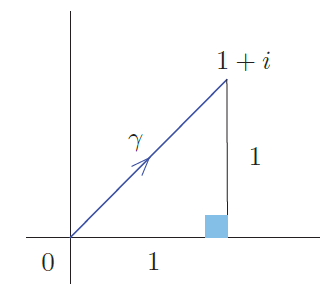
\includegraphics[width=0.3\textwidth]{./Solution/figs/fig-s-0-8}
\end{center}
%\caption{$\left\{ z \in\mathbb C \,:\, z\ne0, \dfrac\pi4 < |\Arg(z)| < \dfrac\pi3 \right\}$}
%\label{fig-5-14}
\end{figure*}

또한 $|(\gamma(t))^2| = |t+it|^2 = 2t^2$이고,
$\max\limits_{t\in[0,1]} |(\gamma(t))^2| = 2\cdot 1^2 = 2$.
따라서
\[
\left| \int_\gamma z^2dz \right|
\le \left( \max\limits_{t\in[0,1]} |(\gamma(t))^2|  \right) \cdot
(\text{$\gamma$의 길이})
= 2\sqrt{2}.
\]
직접 계산하면,
\begin{align*}
\int_\gamma z^2 dz = \int_0^1 (t+it)^2\cdot(1+i)dt
= \int_0^1 (1+i)^3t^2dt = \dfrac{(1+i)^3}3
\end{align*}
이므로
$\left| \dint_\gamma z^2 dz \right| = \dfrac{(\sqrt{3})^3}3 = \dfrac{2\sqrt{2}}3$.

\subsection*{연습문제 \ref{ex-3-10}}

\begin{align*}
{2n \choose n} = \left|  {2n \choose n} \right|
&= \left| \dfrac1{2\pi i}\int_C \dfrac{(1+z)^{2n}}{z^{n+1}}dz \right| \\
&\le \dfrac1{2\pi} \left( \max_{|z|=1} \left| \dfrac{(1+z)^{2n}}{z^{n+1}}\right| \right)
\cdot 2\pi\cdot 1 = \max_{|z|=1} \dfrac{|1+z|^{2n}}1 \\
&\le (1+1)^{2n} = 2^{2n} = 4^n.
\end{align*}

\subsection*{연습문제 \ref{ex-3-11}}

$F=U+iV$를 $\bar z \in \mathbb C$의 부정적분이라고 하자.
그러면,
\[
\dfrac{\partial U}{\partial x}  + i \dfrac{\partial V}{\partial x}
= \dfrac{\partial V}{\partial y} - i\dfrac{\partial U}{\partial y}
= F' = \bar z = x-iy.
\]

$x_0\in\mathbb R$을 고정하자. 그러면 $(x,y)\in\mathbb R^2$에 대하여
\[
V(x,y ) - V(x_0, y) = \int_{x_0}^x \dfrac{\partial V}{\partial x}(\xi, y )d\xi
= \int_{x_0}^x -y d\xi = -xy +x_0y.
\]
따라서 $V(x,y) = -xy + \varphi(y)$, $\varphi(y):+V(x_0,y_0) + x_0y$이면,
\[
x  = \dfrac{\partial V}{\partial y} = -x + \varphi'(y).
\]
즉, 모든 $x\in\mathbb R$에 대하여 $\varphi'(y) = 2x$인데
이는 분명 모순이다.
특히, $2\cdot 1 = 2 = \varphi'(y) = 2\cdot  0 = 0$.

\subsection*{연습문제 \ref{ex-3-12}}

$(fg)' = fg' + f'g$이므로
함수 $\zeta \mapsto f(\zeta)g'(\zeta) + f'(\zeta)g(\zeta)$는 
부정적분을 갖는다.
따라서 경로적분의 기본정리에 의하여
\[
\int_\gamma \left( f(\zeta)g'(\zeta) + f'(\zeta)g(\zeta) \right) d\zeta
= f(z)g(z) - f(w)g(w)
\]
이고 이를 정리하면 원하는 결과를 얻는다.

\subsection*{연습문제 \ref{ex-3-13}}

$\mathbb C$에서 $\sin' z = \cos z$이므로 $\cos z$는 부정적분을 갖는다.
따라서 경로적분의 기본정리에 의하여
\begin{align*}
\int_\gamma \cos z \, dz 
&= \sin i - \sin (-i) = 2\sin i = 2\dfrac{\exp(i\cdot i) - \exp(-i\cdot i)}{2i}
= \dfrac{e^{-1} - e^{1}}i \\
&= \left( e - \dfrac1e \right)i.
\end{align*}


\subsection*{연습문제 \ref{ex-3-14}}

$\mathbb C$에서  $\exp' z = \exp z$이므로
$0$과 $a+ib$를 잇는 경로 $\gamma$를 따라 적분하면
\[
\int_\gamma \exp z\, dz = \exp(a+ib) - \exp 0 = e^a(\cos b + i \sin b) -1
= e^a\cos b -1 +ie^a\sin b.
\]
 경로를 $\gamma(x) = (a+ib)x$, $x\in[0,1]$로 잡으면,
\[
\int_\gamma \exp z\, dz = \int_0^1 \exp(a+ib)\cdot (a+ib)dx
= \int_0^1 e^{ax}(\cos(bx) + i\sin(bx))(a+ib)dx.
\]
 따라서,
$(a-ib)\dint_\gamma \exp z\, dz = \dint_0^1 e^{ax}(\cos(bx) + i\sin(bx))(a^2+b^2)dx$이고,
\begin{align*}
(a^2+b^2) \int_0^1 e^{ax} \cos (bx)dx
&= \Re\left( (a-ib)\int_\gamma \exp z\, dz \right) \\
&= \Re((a-ib)(e^a\cos b -1 + ie^a\sin b)) \\
&= a(e^a\cos b -1) + be^a \sin b.
\end{align*}
즉,
$\dint_0^1 e^{ax}\cos(bx)\, dx = \dfrac{a(e^a\cos b - 1) + be^a\sin b}{a^2+b^2}$.

\subsection*{연습문제 \ref{ex-3-15}}

중심이 $0$이고 반지름 $r>0$인 원을 반시계방향으로 도는 닫힌경로 $C$를 생각하자.
$C(\theta) = r\exp(i\theta)$, $\theta\in[0,2\pi]$.
경로적분의 기본정레에 의해
\begin{align*}
0 & = \int_C \exp z \, dz = \int_0^{2\pi} e^{r\cos\theta +ir\sin\theta}
\cdot ri\exp(i\theta)d\theta\\
&= \int_0^{2\pi} e^{r\cos\theta} \cdot r\cdot i \exp(i(r\sin\theta +\theta))d\theta.
\end{align*}
위 식에서 실수부만 취하면
\[
\int_0^{2\pi} e^{r\cos\theta} \cos(r\sin \theta + \theta)d\theta = 0.
\]

\subsection*{연습문제 \ref{ex-3-16}}

$\mathbb C\setminus\{0\}$에서 복소미분가능한 $F$가 $F'=1/z$를 만족한다고 하자.
중심이 $0$이고 반시계방향으로 도는 원형경로 $C$를 생각하자.
$C$가 닫힌경로 이므로, 경로적분의 기본정리에 의해
\[
\int_C F'(z)dz = 0.
\]
한편, 이미 알고있는 계산 결과에 따르면,
\[
\int_C F'(z)dz = \int_C \dfrac1z dz = 2\pi i
\]
이므로 모순이다.

\subsection*{연습문제 \ref{ex-3-17}}

(ER1)
$\gamma: [0,1] \to D$가 닫힌경로라고 하자.
$H:[0,1]\times[0,1] \to D$를 $H(t,s) = \gamma(t)$, $t,s\in[0,1]$로 정의하면,
$H$는 연속이고,
\begin{align*}
H(t,0) &=\gamma(t), \quad t\in[0,1],\\
H(t,1) &=\gamma(t), \quad t\in[0,1],\\
H(0,s) &=\gamma(0) = \gamma(1) = H(1,s), \quad s\in[0,1].
\end{align*}
따라서 $\gamma$는 자기자신과 $D$-호모토픽하다.
즉, 관계는 반사적(reflexive)이다.
(ER2)
$\gamma_0, \gamma_1: [0,1] \to D$가 닫힌경로이고
$\gamma_0$가 $\gamma_1$과 $D$-호모토픽하다고 하자.
그러면, 다음을 만족하는 연속함수 $H:[0,1]\times[0,1] \to D$가 존재한다.
\begin{align*}
H(t,0) &= \gamma_0(t), \quad t\in [0,1], \\
H(t,1) &= \gamma_1(t), \quad t\in [0,1], \\
H(0,s) &= H(1,s), \quad s\in [0,1].
\end{align*}
$\tilde H:[0,1]\times [0,1] \to D$를
$\tilde H(t,s) = H(t,-s)$, $t,s\in[0,1]$로 정의하자.
그러면, $\tilde H$는 연속이고 다음을 만족한다.
\begin{align*}
\tilde H(t,0) & = H(t,1) = \gamma_1(t), \quad t\in[0,1], \\
\tilde H(t,1) & = H(t,0) = \gamma_0(t), \quad t\in[0,1], \\
\tilde H(0,s) & = H(0,1-s) = H(1,1-s) = \tilde H(1,s), \quad s\in[0,1].
\end{align*}
따라서 $\gamma_1$은 $\gamma_0$와 $D$-호모토픽하다.
즉, 관계는 대칭적(symmetric)이다.

(ER3)
$\gamma_0, \gamma_1, \gamma_2$가 닫힌경로이고
$\gamma_0$가 $\gamma_1$과 $D$-호모토픽하고,
$\gamma_1$이 $\gamma_2$와 $D$-호모토픽하다고 하자.
그러면, 다음을 만족하는 연속함수  $H, K:[0,1]\times[0,1]\to D$가 존재한다.
\begin{align*}
H(t,0) = \gamma_0(t), \ t\in[0,1], \quad & K(t,0) = \gamma_1(t), \ t\in[0,1], \\
H(t,1) = \gamma_1(t), \ t\in[0,1], \quad & K(t,1) = \gamma_2(t), \ t\in[0,1], \\
H(0,s) = H(1,s), \ s\in[0,1], \quad & K(0,s) = K(1,s), \ s\in[0,1].
\end{align*}
$L:[0,1]\times[0,1]\to D$를
\[
L(t,s) = \begin{cases}
H(t,2s), & s\in [0, \frac12], \\
K\left(t, 2(s-\frac12)\right), & s\in (\frac12,1]
\end{cases}
\]
로 정의하면,
\begin{align*}
L(t,0) &= H(t,0) = \gamma_0(t), \quad t\in[0,1],\\
L(t,1) &= K(t,1) = \gamma_2(t), \quad t\in[0,1].
\end{align*}
또한, $0\le s\le \frac12$에 대하여 $L(0,s) = H(0,2s) = H(1,2s) = L(1,s)$, 
$\frac12 <s\le1$에 대하여
\[
L(0,s) = K\left( 0, 2(s - \frac12) \right) = K\left( 1, 2(s - \frac12) \right) = L(1,s).
\]
이다.

$[0,1]\times (\frac12,1]$에서 정의된 수열 $((t_n, s_n))_{n\in\mathbb N}$이
$(t_0,\frac12)$에 수렴한다면,
\begin{align*}
\lim_{n\to\infty} L(t_n, s_n)
& = \lim_{n\to\infty} K\left( t_n, 2(s_n - \frac12)\right)
= K(t_0,0) = \gamma_1(t_0) \\
&= H(t_0,1) = L\left( t_0, \frac12\right) = L\left( \lim_{n\to\infty} (t_n, s_n) \right).
\end{align*}
따라서 $L$은 연속함수이다.
결론적으로, $\gamma_0$는 $\gamma_2$와 $D$-호모토픽하다.
즉, 관계는 추이적(transitive)이다.

이상에서 $D$-호모토피 관계는 반사적, 대칭적, 추이적인 성질을 만족하므로
동치(equivalence) 관계이다.

\subsection*{연습문제 \ref{ex-3-18}}

그림에서 경로 $C$는 경로 $S$와 $\mathbb C\setminus \{0\}$-호모토픽함을 알 수 있다.

\begin{figure*}[h!]
\begin{center}
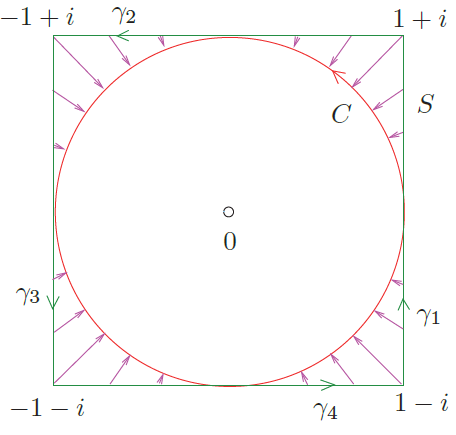
\includegraphics[width=0.4\textwidth]{./Solution/figs/fig-s-0-9}
\end{center}
%\caption{$\left\{ z \in\mathbb C \,:\, z\ne0, \dfrac\pi4 < |\Arg(z)| < \dfrac\pi3 \right\}$}
%\label{fig-5-14}
\end{figure*}

직접 계산을 위해 $t\in[0,1]$에 대하여 경로를 다음과 같이 정의하자.
\begin{align*}
\gamma_1(t) &:= (1-t)(1-i) + t(1+i) = 1 + i(2t-1), \\
\gamma_2(t) &:= (1-t)(1+i) + t(-1+i) = (1-2t) + i, \\
\gamma_3(t) &:= (1-t)(-1+i) + t(-1-i) = -1 + i(1-2t), \\
\gamma_4(t) &:= (1-t)(-1-i) + t(1-i) = 2t-1 -i.
\end{align*}
그러면,
\[
\int_S \dfrac1z dz = \int_{\gamma_1} \dfrac1z dz
+ \int_{\gamma_2} \dfrac1z dz + \int_{\gamma_3} \dfrac1z dz + \int_{\gamma_4} \dfrac1z dz
\]
이므로,
\begin{align*}
\int_{\gamma_1} \dfrac1z dz
&= \int_0^1 \dfrac{2i}{1+i(2t-1)}dt = \int_0^1 \dfrac{2i(1-i(2t-1))}{1+(2t-1)^2}dt \\
&= 2i\int_0^1\dfrac1{1+(2t-1)^2}dt + 2\int_0^1 \dfrac{2t-1}{1+(2t-1)^2}dt \\
&\stackrel{(u=2t-1)}{=} i \int_{-1}^1 \dfrac1{1+u^2}du  + \int_{-1}^1 \dfrac u{1+u^2}du \\
&= i(\tan^{-1}1 - \tan^{-1}(-1)) + 0 
= i\left(\dfrac\pi4 - \left(-\dfrac\pi4\right)\right) = i \dfrac\pi2.
\end{align*}
같은 방법으로, 
\[
\int_0^1 \dfrac2{1+(2t-1)^2}dt = \dfrac\pi2, \quad
\int_0^1 \dfrac{2t-1}{1+(2t-1)^2}dt = 0,
\]
을 이용하면,
\begin{align*}
\int_{\gamma_2} \dfrac1z dz
&= \int_0^1 \dfrac{-2}{1-2t+i}dt = \int_0^1 \dfrac{-2\cdot(-(2t-1)-i)}{1+(2t-1)^2}dt \\
&= 0 + (-1)(-i)\dfrac\pi2 = i\dfrac\pi2, \\
\int_{\gamma_3} \dfrac1z dz
&= \int_0^1 \dfrac{-2i}{-1+i(1-2t)}dt = \int_0^1 \dfrac{-2i\cdot(-1+i(2t-1))}{1+(2t-1)^2}dt \\
&= -i\cdot(-1)\cdot\dfrac\pi2 +0 = i\dfrac\pi2, \\
\int_{\gamma_4} \dfrac1z dz
&= \int_0^1 \dfrac{2}{2t-1-i}dt = \int_0^1 \dfrac{2\cdot((2t-1)+i)}{1+(2t-1)^2}dt \\
&= 0 + i\dfrac\pi2 +0 = i\dfrac\pi2.
\end{align*}
따라서 예상대로 $\dint_S \dfrac1z dz = 4\cdot\left(i\dfrac\pi2\right) = 2\pi i$가 된다.

\subsection*{연습문제 \ref{ex-3-19}}

중심이 $0$이고 반시계방향으로 도는 원형경로 $C$에 대하여
\[
\int_C \dfrac 1z dz = 2\pi i.
\]
한편 그림 \ref{fig-5-17}\과 같이 타원형 경로 $E$는 $C$와 
$\mathbb C\setminus \{0\}$-호모토픽하다.

\begin{figure}[h!]
\begin{center}
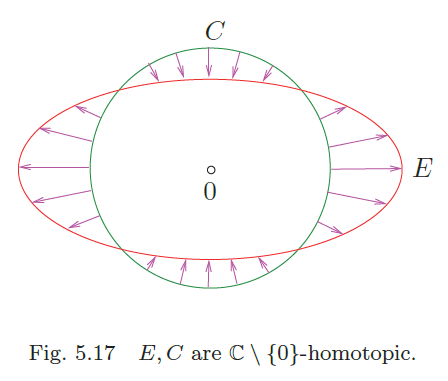
\includegraphics[width=0.4\textwidth]{./Solution/figs/fig-5-17}
\end{center}
\caption{$\mathbb C\setminus \{0\}$-호모토픽한 경로 $E$와 $C$}
\label{fig-5-17}
\end{figure}

따라서 코시 적분정리에 의해 $\dint_E \dfrac 1z dz = \dint_C \dfrac1z dz = 2\pi i$이고,
\begin{align*}
2\pi i &= \int_E \dfrac 1z dz = \int_0^{2\pi} \dfrac1{a\cos\theta +i b\sin\theta}
\cdot(-a\sin\theta + ib\cos\theta)d\theta \\
&= \int_0^{2\pi} \dfrac{(-a\sin\theta +ib\cos\theta)(a\cos\theta -ib\sin\theta)}
{a^2(\cos\theta)^2 + b^2(\sin\theta)^2}d\theta \\
&= \int_0^{2\pi} \dfrac{(b^2-a^2)(\cos\theta)(\sin\theta)+iab((\cos\theta)^2+(\sin\theta)^2)}
{a^2(\cos\theta)^2 + b^2(\sin\theta)^2}d\theta \\
&= \int_0^{2\pi} \dfrac{(b^2-a^2)(\cos\theta)(\sin\theta)+iab\cdot 1}
{a^2(\cos\theta)^2 + b^2(\sin\theta)^2}d\theta.
\end{align*}
허수부를 비교하면,
$\dint_0^{2\pi} \dfrac1{a^2(\cos\theta)^2 + b^2(\sin\theta)^2}d\theta = \dfrac{2\pi}{ab}$.

\subsection*{연습문제 \ref{ex-3-20}}

\begin{figure}[h!]
\begin{center}
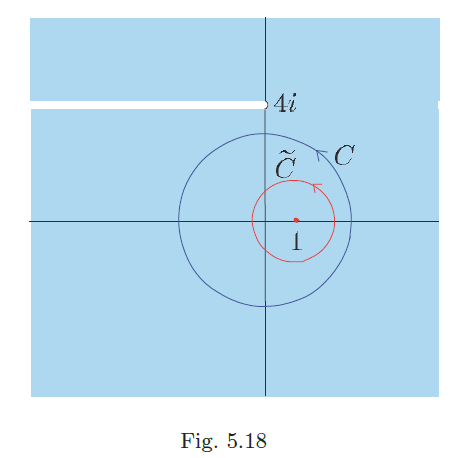
\includegraphics[width=0.4\textwidth]{./Solution/figs/fig-5-18}
\end{center}
\caption{적분경로 $C$, $\tilde C$}
\label{fig-5-18}
\end{figure}

그림 \ref{fig-5-18}을 참고하라.

\begin{itemize}
\item[(1)]  $z\mapsto \Log(z-4i)$는 $\mathbb C \setminus \{r+4i \,:\, r\le0\}$에서
복소해석함수이다. 따라서 코시 적분정리를 쓰면,
\[
\int_C \Log (z-4i)dz = 0.
\]
\item[(2)] $\tilde C$가 중심이 $1$이고 반지름 $r>0$인 원이라 하면,
\[
\int_{\tilde C} \dfrac1{z-1} dz = 2\pi i
\]
임을 알고 있다.
$1/(\cdot -1)$이 $\mathbb C\setminus\{1\}$에서 복소해석함수이고
원형경로 $C$와 $\tilde C$는 $\mathbb C\setminus\{1\}$-호모토픽이므로,
코시 적분정리에 의해,
\[
\int_C \dfrac1{z-1} dz = \int_{\tilde C} \dfrac1{z-1}dz = 2\pi i.
\]
\item[(3)] 
\begin{align*}
i^{z-3} &= \exp((z-3)\Log i) = \exp\left( (z-3)\left( \log 1 + i\dfrac\pi2\right)\right) \\
&= \exp\left( (z-3)\left(0+i\dfrac\pi2\right)\right) \\
&= \exp\left( i\dfrac\pi2 \cdot(z-3)\right).
\end{align*}
따라서 $z\mapsto i^{z-3}$은 전해석함수이다.
코시 적분정리에 의해
\[
\int_C i^{z-3}dz = 0.
\]
\end{itemize}

\subsection*{연습문제 \ref{ex-3-21}}

\begin{itemize}
\item[(1)] 
\[
\varphi'(t) = \exp\left( \int_0^t \dfrac{\gamma'(s)}{\gamma(s)}ds \right)
\cdot \dfrac d{dt}\left( \int_0^t \dfrac{\gamma'(s)}{\gamma(s)}ds \right) 
= \varphi(t)\cdot \dfrac{\gamma'(t)}{\gamma(t)}
\]
에서 $\varphi'\gamma - \varphi\gamma' = 0$이고,
\[
\dfrac d{dt} \left( \dfrac\varphi \gamma \right) 
= \dfrac{\varphi'\gamma - \varphi\gamma'}{\gamma^2} = \dfrac0{\gamma^2} = 0.
\]
따라서 $\dfrac{\varphi(0)}{\gamma(0)}=\dfrac{\varphi(1)}{\gamma(1)}$.
그런데, $\gamma$가 닫힌경로이므로 $\gamma(0)=\gamma(1)$이므로,
\[
\varphi(1) = \varphi(0) = \exp\left( \int_0^0 \dfrac{\gamma'(s)}{\gamma(s)}ds \right)
= \exp(0) = 1.
\]
결론적으로, $w(\gamma) \in\mathbb Z$.
\item[(2)] $\Gamma_1(t) = \exp(2\pi i t)$ ($t\in[0,1]$)의 회전수는
\begin{align*}
w(\Gamma_1) &= \dfrac1{2\pi i} \int_0^1 \dfrac{\Gamma_1'(t)}{\Gamma_1(t)} dt \\
&=\dfrac1{2\pi i} \int_0^1 \dfrac{2\pi i\exp(2\pi i t)}{\exp(2\pi i t)}dt \\
&=\dfrac1{2\pi i} \cdot 2\pi i  = 1.
\end{align*}
\item[(3)]  $(\gamma_1\cdot\gamma_2)'(t) = \gamma_1'(t)\gamma_2(t) +
\gamma_1(t)\gamma_2'(t)$, $t\in[0,1]$이므로,
\begin{align*}
w(\gamma_1\cdot\gamma_2)
&= \dfrac1{2\pi i} 
\int_0^1 \dfrac{(\gamma_1\cdot\gamma_2)'(t)}{(\gamma_1\cdot\gamma_2)(t)}dt\\
&= \dfrac1{2\pi i} \int_0^1 \dfrac{\gamma_1'(t)\gamma_2(t) +\gamma_1(t)\gamma_2'(t)}
{(\gamma_1\cdot\gamma_2)(t)}dt \\
&= \dfrac1{2\pi i} \int_0^1 \dfrac{\gamma_1'(t) \cancel{\gamma_2(t)}}
{\gamma_1(t) \cancel{\gamma_2(t)}}dt 
+ \dfrac1{2\pi i} \int_0^1 \dfrac{\cancel{\gamma_1(t)}\gamma_2'(t)}
{\cancel{\gamma_1(t)}\gamma_2(t)}dt  \\
&= w(\gamma_1) + w(\gamma_2).
\end{align*}
\item[(4)] $\Gamma_m = \Gamma_1 \cdot\cdots\cdot \Gamma_1$ ($m$번 곱)이므로
\begin{align*}
w(\Gamma_m) &= w(\Gamma_1) + \cdots + w(\Gamma_1) \ \ (m\text{번}) \\
&= m\cdot w(\Gamma_1) = m\cdot 1 = m.
\end{align*}
\item[(5)] 함수 $\varphi:[0,1]\to \mathbb R$를 
원점에서 $\gamma_0(t)$까지의 거리 $\varphi(t) = |\gamma_0(t)|$, $t\in[0,1]$로 정의하자.
$\gamma_0$가 $0$을 지나지 않고, $\varphi$는 연속함수이기 때문에
최솟값 $d_0$ ($d_0>0$)를 갖는다.
$\delta = d_0/2 >0$로 택하자.
$\gamma$가 
\[
\|\gamma - \gamma_0\| := \max_{t\in[0,1]} | \gamma(t) - \gamma_0(t)| < \delta
\]
를 만족하는 매끄러운 닫힌경로라고 하자.
그러면
$\gamma$가 $\gamma_0$와 $\mathbb C\setminus \{0\}$-호모토픽함을 증명하고자 한다.
$H:[0,1]\times[0,1]\to \mathbb C\setminus\{0\}$를 
$H(t,s) = (1-s)\gamma_0(t) + s\gamma(t)$, $t,s\in[0,1]$로 정의하면
$H$는 연속함수이고,
\begin{align*}
H(t,0) &= \gamma_0(t), \quad t\in[0,1],\\
H(t,1) &= \gamma(t), \quad t\in[0,1],\\
H(0,s) &= (1-s)\gamma_0(0) + s\gamma(0) \\
&= (1-s)\gamma_0(1) + s\gamma(1)  = H(1,s), \quad s\in[0,1].
\end{align*}

또한, $H(t,s)$는 $0$이 될 수 없다. 왜냐하면,
$\gamma_0(t)$와 $\gamma(t)$의 볼록결합이기 때문이다.
어떤 $t,s$에 대하여 $(1-s)\gamma_0(t)+s\gamma(t)=0$라면
모순에 도달하게 된다. 그림 \ref{fig-5-19}\를 참고하라.

\begin{figure}[h!]
\begin{center}
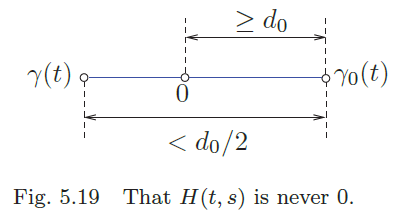
\includegraphics[width=0.4\textwidth]{./Solution/figs/fig-5-19}
\end{center}
\caption{$H(t,s)$는 $0$이 될 수 없다.}
\label{fig-5-19}
\end{figure}
직접 계산해보면,
\begin{align*}
1\cdot \dfrac{d_0}2 &> s|\gamma_0(t) - \gamma(t)|
= | \gamma_0(t) - 
\underbrace{((1-s)\gamma_0(t) + s\gamma(t))}_{=0\text{인 $t,s$를 선택할 수 있다면}}
| = |\gamma_0(t) - 0| \\
&= |\gamma_0(t)| \ge d_0.
\end{align*}
그러면, 코시 적분정리에 의해
\[
w(\gamma) = \dfrac1{2\pi i} \int_\gamma \dfrac1z dz 
= \int_{\gamma_0} \dfrac1z dz  = w(\gamma_0).
\]
\end{itemize}

\subsection*{연습문제 \ref{ex-3-22}}

\begin{figure*}[h!]
\begin{center}
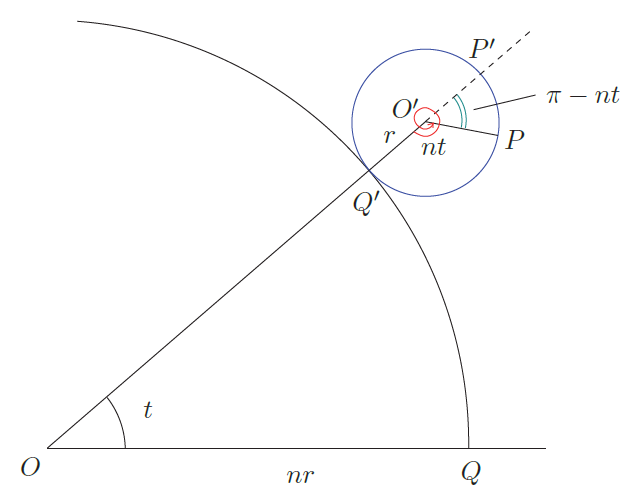
\includegraphics[width=0.4\textwidth]{./Solution/figs/fig-s-0-10}
\end{center}
%\caption{적분경로 $C$, $\tilde C$}
%\label{fig-5-18}
\end{figure*}

\begin{itemize}
\item[(1)] 큰 원의 각 $\angle Q'OQ$에 대응하는 호의 길이는 $t\cdot nr$이다.
작은 동전이 미끄러지지 않고 돌아갈 때, $O'P$와 $OO'$이 이루는 각은
$(t\cdot nr)/r = n\cdot t$이다. 그림에서 $O' \equiv (nr+r)\exp(it)$이고
\begin{align*}
P & \equiv (nr+r)\exp(it) + 
\underbrace{\exp(-i(\pi-nt))}_{\text{시계방향으로 회전}}\cdot
\underbrace{r\exp(it)}_{O'P'} \\
&=(n+1)r\exp(it) + (-1)\cdot r\cdot \exp((n+1)it).
\end{align*}
\item[(2)] 에피사이클로이드 곡선 $\gamma$로 둘러싸인 영역의 면적은
 \begin{align*}
\dfrac1{2i} \int_\gamma \bar z dz 
&= \dfrac1{2i}\int_0^{2\pi} \overline{r\left( (n+1)\exp(it)-\exp((n+1)it)\right)}\cdot \\
&\qquad\qquad r\left((n+1)i\exp(it) - (n+1)i\exp((n+1)it)\right)dt \\
&= \dfrac1{2i} \int_0^{2\pi} r^2\left( (n+1)\exp(-it) - \exp(-(n+1)it)\right)\cdot  \\
&\qquad\qquad (n+1)i\left(\exp(it) - \exp((n+1)it)\right)dt \\
&= \dfrac{(n+1)r^2}2 \int_0^{2\pi} ((n+1) -(n+1)\exp(int) - \exp(-int) +1)dt \\
&= \dfrac{(n+1)r^2}2 ((n+1) \cdot 2\pi + 0+0 + 2\pi) \\
&= (n+1)r^2\pi(n+2) = \pi r^2 (n+1)(n+2).
\end{align*}
\end{itemize}

\subsection*{연습문제 \ref{ex-3-23}}

$z\in D:= \mathbb C\setminus\{0\}$에 대하여 $f(z) = 1/z$로 정의하자.
그러면, $f$는 $D$에서 부정적분(원시함수)을 가질 수 없다.
(예제 \ref{example-3-7}\과 연습문제 \ref{ex-3-16 }\을 참고하라.)

\subsection*{연습문제 \ref{ex-3-24}}

$\gamma(t) = \exp(it)$, $t\in[0,1]$이라 하면,
\begin{align*}
\int_\gamma \dfrac i{(z-a)(az-1)}dz 
&= \int_0^{2\pi} \dfrac{i}{(\exp(it) -a)(a\exp(it)-1)}i\exp(it)dt \\
&= \int_0^{2\pi} \dfrac{-\exp(it)}{(\exp(it) -a)(a-\exp(-it))\exp(it)}dt \\
&= \int_0^{2\pi} \dfrac{1}{(\exp(it) -a)(\exp(-it)-a)}dt \\
&= \int_0^{2\pi} \dfrac1{|\exp(it)-a|^2}dt \\
&= \int_0^{2\pi} \dfrac1{((\cos t)-a)^2 + (\sin t)^2}dt \\
&= \int_0^{2\pi} \dfrac1{1-2a\cos t + a^2}dt.
\end{align*}
$0<a<1$일 때,
함수 $z\mapsto i/(ax-1)$이 단위원 $\gamma$를 포함하는 원판에서 복소해석함수이므로,
코시 적분공식에 의해
\[
\dfrac1{2\pi i} \int_\gamma \dfrac{\frac{i}{az-1}}{z-a}dz = \dfrac{i}{az-1}\Big|_{z=a}
= \dfrac i{a^2-1}.
\]
따라서,
$\dint_0^{2\pi} \dfrac 1{1-2a\cos t +a^2}dt
= \dint_\gamma \dfrac{\frac{i}{az-1}}{z-a}dz 
= 2\pi i \cdot \dfrac i{a^2-1} = \dfrac{2\pi}{1-a^2}$.

\subsection*{연습문제 \ref{ex-3-25}}

\begin{figure*}[h!]
\begin{center}
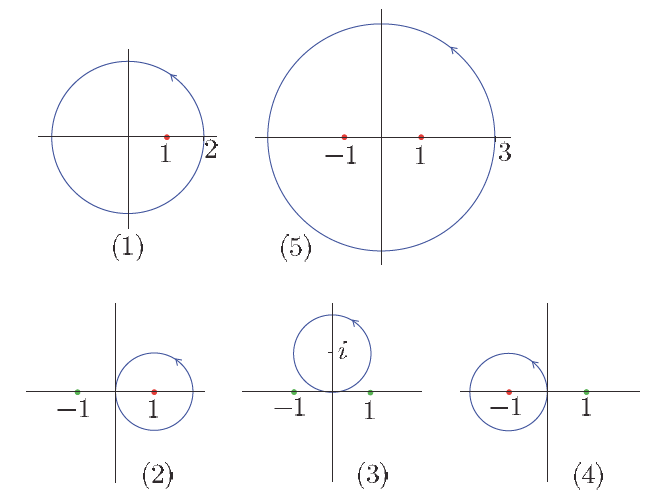
\includegraphics[width=0.7\textwidth]{./Solution/figs/fig-s-0-11}
\end{center}
%\caption{적분경로 $C$, $\tilde C$}
%\label{fig-5-18}
\end{figure*}

\begin{itemize}
\item[(1)] $\dint_\gamma \dfrac{\exp z}{z-1}dz = 2\pi i \exp z \Big|_{z=1}
= 2\pi i \exp 1 = 2\pi i  e$.
\item[(2)] $\dint_\gamma \dfrac{z^2+1}{z^2-1}dz 
= \dint_\gamma \dfrac {\frac{z^2+1}{z+1}}{z-1}dz
= 2\pi i \dfrac{z^2+1}{z+1} \Big|_{z=1} = 2\pi i \dfrac{1^2+1}{1+1} = 2\pi i$.
\item[(3)] $\dint_\gamma \dfrac{z^2+1}{z^2-1}dz = 0$.
\item[(4)] $\dint_\gamma \dfrac{z^2+1}{z^2-1}dz 
= \dint_\gamma \dfrac{\frac{z^2+1}{z-1}}{z-(-1)}dz 
= 2\pi i \dfrac{z^2+1}{z-1} \Big|_{z=-1} = 2\pi i \dfrac{(-1)^2+1}{-1-1} = -2\pi i$.
\item[(5)] $\dint_\gamma \dfrac{z^2+1}{z^2-1}dz 
= \dint_\gamma \dfrac{z^2+1}2 \left(\dfrac1{z-1} - \dfrac1{z+1}\right)dz$
\begin{align*}
\quad &= \int_\gamma \dfrac{\frac{z^2+1}2}{z-1}dz 
- \int_\gamma \dfrac{\frac{z^2+1}2}{z-(-1)}dz 
= 2\pi i \dfrac{z^2+1}2\Big|_{z=1} - 2\pi i \dfrac{z^2+1}2 \Big|_{z=-1} \\
&= 2\pi i(1) - 2\pi i (1) = 0.
\end{align*}
\end{itemize}

\subsection*{연습문제 \ref{ex-3-26}}

$F$가 부정적분이라고 하자.
원 $|z-0| = \frac12$을 반시계방향으로 도는 닫힌경로 $\gamma$를 생각하자.
경로적분의 기본정리에 의해,
\[
\dint_\gamma \dfrac1{z(z^2-1)}dz = \int_\gamma F'(z)dz = 0.
\]
한편,  코시 적분공식을 쓰면,
\[
\int_\gamma \dfrac1{z(z^2-1)}dz = \int_\gamma  \dfrac{\frac1{z^2-1}}{z-0}dz
= 2\pi i \dfrac1{z^2-1}\Big|_{z=0} = 2\pi i \dfrac1{0^2-1} = - 2\pi i.
\]
따라서 모순에 도달하게 되어
\[
\dfrac1{z(z^2-1)}
\]
은 $\{z\in\mathbb C\,:\, 0<|z|<1\}$에서 부정적분을 가질 수 없다.

\subsection*{연습문제 \ref{ex-3-27}}

\begin{figure}[h!]
\begin{center}
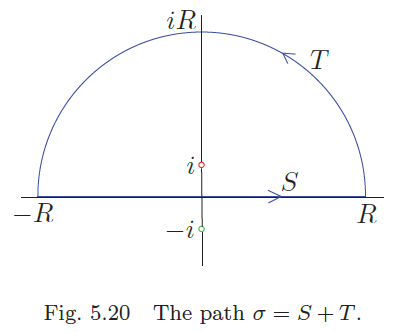
\includegraphics[width=0.4\textwidth]{./Solution/figs/fig-5-20}
\end{center}
\caption{경로 $\sigma=S+T$}
\label{fig-5-20}
\end{figure}

\begin{itemize}
\item[(1)] 코시 적분공식에 의해
\begin{align*}
\int_\sigma F(z) dz &= \int_\sigma \dfrac{\exp(iz)}{z^2+1}dz
= \int_\sigma \dfrac{\frac{\exp(iz)}{z+1}}{z-1}dz
= 2\pi i \dfrac{\exp(iz)}{z+1}\Big|_{z=i} \\
&= 2\pi i \dfrac{\exp(i\cdot i)}{i+i} = 2\pi i \dfrac{e^{-1}}{2i} = \dfrac\pi e.
\end{align*}

\item[(2)] $z=x+iy$, $x,y$는 실수이고, $y\ge0$라 하자. 그러면,
\[
|\exp(iz)| = |\exp(i(x+iy))| = |\exp(-y+ix)| = e^{-y} \le 1.
\]
따라서,
\[
|F(z)| = \dfrac{|\exp(iz)|}{|z^2+1|} \le \dfrac1{|z^2+1|}.
\]
한편, $|z^2| - |-1| \le |z^2-(-1)| = |z^2+1|$이므로,
$|z|\ge\sqrt{2}$이면,
\[
|F(z)| \le \dfrac1{|z^2+1|} \le \dfrac1{|z|^2-1} \le \dfrac2{|z|^2}.
\]
부등식을 만들 때 $|z^2|\ge 2$이면, $|z|^2\le 2|z|^2 -2$임을 이용하였다.
($|z|\ge\sqrt{2}$이면 이 조건이 만족된다)
\item[(3)] 
\begin{align*}
\left| \int_T F(z)dz \right| 
\le 2\pi R\cdot \max_{z\in T} |F(z)| &\le 2\pi R\cdot \dfrac 2{R^2} 
\quad (R\ge\sqrt{2}\text{일 때})\\
&= \dfrac{4\pi}R \stackrel{R\to\infty}{\longrightarrow} 0.
\end{align*}
따라서 $\Lim_{R\to\infty} \int_T F(z) dz = 0$.
\[
\int_S F(z)dz = \int_\sigma F(z) dz - \int_T F(z)dz = \dfrac \pi 2 -  \int_T F(z)dz
\]
이므로,  $\Lim_{R\to\infty} \int_S F(z)dz = \dfrac\pi e -\Lim_{R\to\infty} \int_T F(z)dz
= \dfrac \pi e - 0 = \dfrac \pi e$.
\item[(4)] $S(x)=x$, $x\in[-R,R]$이라 하자. 그러면,
\begin{align*}
\int_S F(z)dz &= \int_{-R}^R \dfrac{\exp(ix)}{x^2+1}\cdot 1 dx
=\int_{-R}^R \dfrac{\cos x}{x^2+1} dx 
+ i\int_{-R}^R \dfrac{\sin x}{x^2+1} dx \\
&= \int_{-R}^R \dfrac{\cos x}{x^2+1}dx  + 0
\end{align*}
마지막 등식은 $\dfrac{\sin x}{x^2+1}$이 기함수라는 성질을 이용하였다.
결론적으로,
\[
\Lim_{R\to\infty} \int_{-R}^R \dfrac{\cos x}{x^2+1}dx
= \Lim_{R\to\infty}\int_S F(z)dz = \dfrac \pi e.
\]
\end{itemize}

\subsection*{연습문제 \ref{ex-3-28}}

전해석함수 $\exp z$와 중심이 $0$이고 빈지름 $1$인 원형경로
$C:[0,2\pi] \to \mathbb C$가 $C(\theta) = \exp(i\theta)$, $\theta \in [0,2\pi]$로 
주어졌다고 하자.
코시  적분공식에 의하여,
\[
\dfrac1{2\pi i} \int_C \dfrac{\exp z}{z-0}dz = \exp z\Big|_{z=0} = \exp 0 = 1.
\]

한편,
\begin{align*}
\int_C \dfrac{\exp z}{z-0}dz 
&= \int_0^{2\pi} \dfrac{\exp(\exp(i\theta))}{\exp(i\theta)}\cdot i{\exp(i\theta)}d\theta
= i \int_0^{2\pi}  \exp(\exp(i\theta))d\theta \\
&=i \int_0^{2\pi}   \exp(\cos\theta +i\sin\theta)d\theta\\
&= i \int_0^{2\pi}  e^{\cos\theta} (\cos(\sin\theta) + i\sin(\sin\theta))d\theta\\
&= - i \int_0^{2\pi}   e^{\cos\theta} \sin(\sin\theta)d\theta 
+ i \int_0^{2\pi}     e^{\cos\theta} \cos(\sin\theta)d\theta.
\end{align*}
따라서,
$\dint_0^{2\pi} e^{\cos\theta} \cos(\sin\theta)d\theta = 2\pi$.

\subsection*{연습문제 \ref{ex-3-29}}

$f$가 복소해석함수이면, $f^{(n)}$도 복소해석함수이다.
따라서 복소미분 $f^{(n+1)}$이 존재한다.
또한, $f^{(n+1)}$이 복소미분가능하므로, 연속함수도 된다.
즉, $f^{(n)}$이 연속적으로 복소미분가능하다.

\subsection*{연습문제 \ref{ex-3-30}}

모든 $ z\in \mathbb C$에 대하여
$|f(z)| \ge \delta >0$이라고 하자.
특히, 모든 $z\in\mathbb C$에서 $f(z)\ne0$이므로
$1/f$는 전해석함수가 된다.
그런데 모든 $z\in\mathbb C$에 대하여
\[
\left| \dfrac1{f(z)}\right| \le \dfrac1\delta
\]
이므로 리우비유 정리에 의해 $1/f$는 상수함수가 되어,
$f$도 상수함수가 된다.

\subsection*{연습문제 \ref{ex-3-31}}

$z\in\mathbb C$에 대하여 $g(z):= f(z) - w_0$로  정의하자.
그러면, $g$는 전해석함수이고, 모든 $z\in\mathbb C$에 대하여  $|g(z)|\ge r$이다.
따라서 $g$는 원점에서 일정한 거리만큼 떨어져 있다.
연습문제 \ref{eq-3-30}에 의하여 $g$는 상수함수가 되므로,
$f = g +w_0$도 상수함수이다.

\subsection*{연습문제 \ref{ex-3-32}}

콤팩트 집합 $K:=\{ (x,y) \,:\, 0\le x\le T_1, 0\le y \le T_2\}$를 생각하자.
그러면 연속함수 $(x,y)\mapsto |f(x+iy)|$는 $K$에서 최댓값을 갖는다. 
최댓값을  $M$이라 하자. 
실수의 집합을 구간으로 나누면
\[
x,y\in\mathbb R = \bigcup_{n\in\mathbb Z} [ nT_1, (n+1)T_1)
= \bigcup_{m\in\mathbb Z} [ mT_1, (m+1)T_1)
\]
$x+iy = x_0 +nT_1 + i(y_0+mT_2)$을 만족하는 정수 $m$, $n$과
실수 $x_0\in [0,T_1)$, $y_0\in [0,T_2)$가 존재한다.
함수 $f$의 주기성으로부터 모든 $x,y\in\mathbb R$에 대하여
\[
f(x+iy) = f(x_0+nT_1 + i(y+0+mT_2)) = f(x_0+iy_0) \in f(K)
\]
이고, $|f(x_0+iy_0)| \le M$이다.
따라서 $f$는 $\mathbb C$ 전체에서 유계이고
리우비유 정리에 의해 상수함수가 된다.

\subsection*{연습문제 \ref{ex-3-33}}

\begin{itemize}
\item[(1)] $z\in\mathbb C$에서 $g(z)=\exp(z)\cdot f(z)$라고 정의하면
$g$는 전해석함수이다. $|f(z)| \le|\exp z|$이므로 모든 $z\in\mathbb C$에 대하여
\[
|g(z)| =| \exp(-z)\cdot f(z)| \le 1.
\]
리우비유 정리에 의해 $g$는 상수함수가 되고, 상수를 $c$라 하면,
$|g(z)|\le1$로부터 $|c|\le1$이고,
\[
g(z) = \exp(-z)\cdot f(z) = c
\]
이므로 모든 $z\in\mathbb C$에 대하여 $f(z)  = c\cdot \exp z$이다 ($|c|\le1$).

\item[(2)] $p$가 차수 $d\ge1$의 다항식이면,
$|z|>R$에 대하여
\[
|p(z)| \ge M|z|^d
\]
를 만족하는 $M, R>0$이 존재한다.
$z=x <  -R <0$로 선택하면,
$|z|>R$이고, $M|x|^d \le |p(z)| \le |e^x| = e^x \le 1$이다 ($x<0$이므로).
따라서 모든 $x<-R$에 대하여 $|x|^d \le 1/M$이 되어 모순이다.
이제 $p$가 상수함수가 되므로 상수를 $c_0$라 하자.
다시 $|p(z)| \le |\exp z|$로부터 $z=x<0$로 두면
임의의 $x<0$에 대하여
$|c_0| \le |e^x| = e^x$가 되어 $|c_0|=0$이다.
결론적으로 $p=c_0=0$을 얻는다.
\end{itemize}

\subsection*{연습문제 \ref{ex-3-34}}

\begin{itemize}
\item[(1)] $z\in C$에 대하여
\begin{align*}
|z-a_1| &\ge |z| - |a_1| = R - |a_1|, \\
|z-a_2| &\ge |z| - |a_2| = R - |a_2|
\end{align*}
이므로 
\begin{align*}
\left| \int_C \dfrac{f(z)}{(z-a_1)(z-a_2)} dz \right|
&\le \max_{z\in\mathbb C} \dfrac|{f(z)|}{|z-a_1| |z-a_2|} \cdot
(C\text{의 길이}) \\
&\le \dfrac{M}{(R-|a_1|)(R-|a_2|)}\cdot 2\pi R
\end{align*}
단, $M:= \max\limits_{z\in\mathbb C}|f(z)|$.

\item[(2)]  $a_1\ne a_2$이므로
\[
\dfrac1{z-a_1} - \dfrac1{z-a_2} = \dfrac{z-a_2 -(z-a_1)}{(z-a_1)(z-a_2)}
= \dfrac{a_1 -a_2}{(z-a_1)(z-a_2)}
\]
이고
\[
\dfrac1{(z-a_1)(z-a_2)} = \dfrac1{a_1 - a_2} \left(
\dfrac1{z-a_1} - \dfrac1{z-a_2} \right)
\]
이다. 따라서 $\alpha:=-\beta:= \dfrac1{a_1-a_2}$이다.

\item[(3)] 
\begin{align*}
\int_C \dfrac{f(z)}{(z-a_1)(z-a_2)} dz
&= \int_C \dfrac1{a_1-a_2}\left(
\dfrac1{f(z)}{z-a_1} - \dfrac{f(z)}{z-a_2} \right) dz \\
&= \dfrac1{a_1-a_2} \left( \int_C \dfrac{f(z)}{z-a_1}dz - \int_C \dfrac{f(z)}{z-a_2}dz \right).
\end{align*}
중심이 $a_1$이고 반지름 $r_1>0$인 원 $C_1$을 둘레로 하는 작은 원판 $ \Delta_1$을 생각하자.
그러면 $C$와 $C_1$은 $\mathbb C \setminus \{a_1\}$-호모토픽하고
\[
g(z):= \dfrac{f(z)}{z-a_1}, \quad z\in \mathbb C\setminus \{a_1\}
\]
는 복소해석함수이다. 코시 적분정리에 의해
\[
\int_C \dfrac{f(z)}{z-a_1}dz = \int_{C_1} \dfrac{f(z)}{z-a_1}dz.
\]
한편, 코시 적분공식을 쓰면,
$\dfrac1{2\pi i} \dint_{C_1} \dfrac{f(z)}{z-a_1}dz = f(a_1)$이므로
\[
\int_C \dfrac{f(z)}{z-a_1}dz = 2\pi i f(a_1).
\]
같은 방법으로
\[
\int_C \dfrac{f(z)}{z-a_2}dz = 2\pi i f(a_2).
\]
종합하면, $\dint_C \dfrac{f(z)}{(z-a_1)(z-a_2)} dz
= \dfrac{2\pi i(f(a_1) - f(a_2))}{a_1 - a_2}$.
\item[(4)]
$f$가 유계인 전해석함수이고 $|f|$는 상계 $M$을 갖는다고 가정하자.
즉, 모든 $z\in\mathbb C$에 대하여 $|f(z)| \le M$이다.
$a_1, a_2$가 $\mathbb C$의 서로 다른  두 점이라고 하자.
중심이 $0$이고 반지름 $R>0$인 원을 반시계방향으로 도는 경로 $C$가
$a_1, a_2$를 내부에 포함하도록 잡을 수 있다.
앞의 (1), (3)의 결과를 이용하면,
\begin{align*}
|f(a_1) - f(a_2)|
&= \dfrac{|a_1 - a_2|}{2\pi} \cdot \left| \dfrac{2\pi i(f(a_1) - f(a_2))}{a_1 - a_2} \right| \\
&= \dfrac{|a_1 - a_2|}{2\pi} \cdot \left| \int_C \dfrac{f(z)}{(z-a_1)(z-a_2)}dz \right| \\
&\le \dfrac{|a_1 - a_2|}{2\pi} \cdot \dfrac{2\pi RM}{(R-|a_1|)(R-|a_2|)}.
\end{align*}
$R$은 원하는 만큼 크게 잡을 수 있으므로, 
$R\to\infty$에 따라
\[
\dfrac{2\pi RM}{(R-|a_1|)(R-|a_2|)} \to 0
\]
이므로 $|f(a_1) - f(a_2)| =0$이다.
따라서 $f(a_1) = f(a_2)$로부터 $f$는 상수함수이다.
\end{itemize}










 

%===[salt] 4장
% !TEX root = ../CA_book.tex

\section*{4장 - 연습문제 풀이}

\subsection*{연습문제 \ref{ex-4-1}}

$\Sum_{n=1}^\infty a_n$이 수렴하면,
$\Sum_{n=1}^\infty \Re(a_n)$과 $\Sum_{n=1}^\infty \Im(a_n)$도 각각 수렴한다.
따라서 $\Lim_{n\to\infty} \Re(a_n) = 0$이고, $\Lim_{n\to\infty} \Im(a_n) = 0$이다.
이로부터 $\Lim_{n\to\infty} a_n = 0$이다.

\subsection*{연습문제 \ref{ex-4-2}}

$\Sum_{n=1}^\infty |a_n|$이 수렴한다고 하자.
모든 $ n\in \mathbb N$에 대하여
$\Re(a_n) \le |a_n|$, $\Im(a_n) \le |a_n|$이므로
비교판정법에 의해
\[
\Sum_{n=1}^\infty \Re(a_n), \quad \Sum_{n=1}^\infty \Im(a_n)
\]
이 수렴한다.
따라서 $\Sum_{n=1}^\infty a_n$도 수렴한다.

\subsection*{연습문제 \ref{ex-4-3}}

$s_n:= 1+z+\cdots + z^{n-1}+z^n$이라 하면,
$z s_n = z + z^2 + \cdots + z^n + z^{n+1}$이므로
$(1-z)s_n = 1- z^{n+1}$이다.
$|z|<1$에서  $z\ne1$이므로
\begin{equation}\label{eq-5-21}
s_n = 1+z+\cdots + z^{n-1}+z^n = \dfrac{1-z^{n+1}}{1-z}.
\end{equation}
따라서
\[
\Lim_{n\to\infty} s_n = \lim_{n\to\infty}\dfrac{1-z^{n+1}}{1-z}
= \dfrac{1-0}{1-z} = \dfrac1{1-z}
\]
이므로 $\Sum_{n=0}^\infty z^n$이 수렴하고
$\Sum_{n=0}^\infty z^n = \Lim_{n\to\infty} s_n = \dfrac1{1-z}$이다. \\[1ex]
(이 증명을 위해 $|z|<1$에서
\[
\lim_{n\to\infty} z^{n+1} = 0
\]
을 이용하였다.  이 결과는
$r:=|z|<1$이므로, $|z^{n+1} -0| = |z|^{n+1} \stackrel{n\to\infty}{\longrightarrow }0$으로부터
얻어진다.)

\subsection*{연습문제 \ref{ex-4-4}}

자연수 $n\in\mathbb N$에 대하여 
$s_n:= 1+2z + 3z^2 + \cdots + (n-1)z^{n-2} + nz^{n-1}$이라 하자.
그러면 $zs_n = z + 2z^2 + \cdots + (n-1)z^{n-1} + nz^n$이다.
따라서
\[
(1-z)s_n= 1 + z + z^2 + \cdots + z^{n-1} - nz^n
= \dfrac{1-z^n}{1-z}  - nz^n.
\]
따라서
\[
s_n = \dfrac{1-z^n}{(1-z)^2}  - \dfrac{nz^n}{1-z}.
\]
(이 결과는 식 \eqref{eq-5-21}의 양변을 $z$에 대하여 미분해서 얻을 수도 있다.)

$r:=|z|$ ($0\le r < 1$)이라 하면,
\[
r = \dfrac1{1+h}
\]
여기서 $h:=\dfrac1r-1>0$이다.
\[
(1+h)^n = 1 + {n\choose 1}h + {n \choose 2}h^2 + \cdots
+ {n \choose n}h^n \ge {n \choose 2}h^2 = \dfrac{n\cdot(n-1)}2 \cdot h^2
\]
에서
\[
0\le nr^n = \dfrac n{(1+h)^n} \le n \cdot \dfrac2{n\cdot(n-1)\cdot h^2}
= \dfrac 2{(n-1)\cdot h^2}
\]
이므로
조임정리(Sandwitch theorem)에 의하여 $\Lim_{n\to\infty} nr^n = 0$이다.
결론적으로,
\[
\Lim_{n\to\infty}  s_n = \Lim_{n\to\infty} \left( \dfrac{1-z^n}{(1-z)^2}
- \dfrac{nz^n}{1-z} \right)
= \dfrac{1-0}{(1-z)^2} - \dfrac0{1-z} = \dfrac1{(1-z)^2}.
\]

\subsection*{연습문제 \ref{ex-4-5}}

\begin{align*}
\left| \dfrac1{n^s} \right| &= \left| \dfrac1{\exp(s\cdot \Log(n))} \right|
= \left| \dfrac1{\exp(s\cdot\log n)}\right| \\
&= \dfrac1{e^{\Re(s\cdot \log n)}} = \dfrac1{e^{(\log n)\cdot(\Re(s))}}
= \dfrac1{(e^{\log n})^{\Re(s)}} = \dfrac1{n^{\Re(s)}}.
\end{align*}

$p>1$\,일 때 $\Sum_{n=1}^\infty \dfrac1{n^p}$이 수렴함을 이용하면,
$\Re(s)>1$에 대하여
\[
\sum_{n=1}^\infty \dfrac1{n^{\Re(s)}}
\]
가 수렴한다. 따라서  $\Re(s)>1$인 영역에서
\[
\sum_{n=1}^\infty \dfrac1{n^{s}}
\]
은 절대수렴하므로, 당연히 수렴한다.

\subsection*{연습문제 \ref{ex-4-6}}

$L\ne0$이라고 하자.
$|z|< 1/L$인 모든 $z$에 대하여, 
$N$이 충분히 클 때 $n>N$이면
$\sqrt[n]{|c_nz^n|}  = \sqrt[n]{|c_n|}|z| \le q <1$를 만족하는 $q<1$가 존재한다. 
이 결과는 $\sqrt[n]{|c_n|}|z| \xrightarrow{n\to\infty} L|z|<1$로부터 얻어진 것이다.
(예를 들어 $q=(L|z|+1)/2 <1$로 잡으면 된다.)

$L=0$이면, 
임의의(고정된) $z\in \mathbb C$에 대하여
$n>N$이면 $\sqrt[n]{|c_nz^n|} = \sqrt[n]{|c_n|}|z| \le q < 1$을 항상 만족하는 $q<1$가 존재한다.
이 결과는  $\sqrt[n]{|c_n|}|z| \xrightarrow{n\to\infty} 0|z|=0<1$로부터 얻어진다.
(예를 들어 $q=1/2<1$로 잡으면 된다.)
근판정법(root test)\footnote{
역주:
급수 $\Sum a_n$에 대하여
극한 $L = \Lim_{n\to\infty} \sqrt[n]{|a_n|}$이 존재할 때,
$L<1$이면 급수가 수렴하고
$L>1$이면 급수가 발산한다.
}을 쓰면 제곱급수가 수렴함을 알 수 있다.

한편, $L\ne0$이고 $|z|>1/L$인 경우를 생각하면
$N$이 충분히 클 때 모든 $n>N$에 대하여
$\sqrt[n]{|c_nz^n|}  = \sqrt[n]{|c_n|}|z| >1$가 성립한다.
이 결과는  $\sqrt[n]{|c_n|}|z| \xrightarrow{n\to\infty} L|z|>1$로부터 얻어진다.
다시 근판정법을 쓰면 이 경우 제곱급수가 발산함을 알 수 있다.

\subsection*{연습문제 \ref{ex-4-7}}

$z=0$일 때 급수가 $0$으로 수렴함은 자명하다.
$z\ne 0$라고 가정하자. 그러면, $N>1/|z|$인 
$N\in\mathbb N$를 선택할 수 있다.
$n>N$에 대하여 $|nz|>N|z|>1$이고
$|n^nz^n -0| = |nz|^n >1^n = 1$이므로
\[
\neg \left( \lim_{n\to\infty} n^n z^n = 0 \right).
\]
따라서 $z\ne0$이면, $\Sum_{n=1}^\infty n^n z^n$은 발산한다.

\subsection*{연습문제 \ref{ex-4-8}}

$\Lim_{n\to\infty} \sqrt[n]{\dfrac1{n^n}} = \Lim_{n\to\infty} \dfrac1n = 0$이므로
\[
\sum_{n\to\infty} \dfrac{z^n}{n^n}
\]
의 수렴 반지름은 무한대이고 이 제곱급수는 모든 $z\in\mathbb C$에 대하여 수렴한다.

\subsection*{연습문제 \ref{ex-4-9}}

\begin{itemize}
\item[(1)] 
\[
\lim_{n\to\infty} \left| \dfrac{\dfrac{(-1)^{n+1}}{n+1}}{\dfrac{(-1)^n}n} \right|
= \lim_{n\to\infty} \dfrac n{n+1} = 1
\]
이므로 $\Sum_{n=1}^\infty \dfrac{(-1)^n}n z^n$의 수렴 반지름은 $1$이다.

\item[(2)] 
\[
\lim_{n\to\infty} \left| \dfrac{(n+1)^{2012}}{n^{2012}} \right|
= \lim_{n\to\infty} \left( 1+ \dfrac1{n} \right)^{2012} = 1
\]
이므로 $\Sum_{n=1}^\infty n^ {2012} z^n$의 수렴 반지름은 $1$이다.

\item[(3)] 
\[
\lim_{n\to\infty} \left| \dfrac{\dfrac{1}{(n+1)!}}{\dfrac1{n!}} \right|
= \lim_{n\to\infty} \dfrac1{n+1} = 0
\]
이므로 $\Sum_{n=1}^\infty \dfrac1{n!}z^n$의 수렴 반지름은 무한대이다.
\end{itemize}

\subsection*{연습문제 \ref{ex-4-10}}

$|z|<1$에 대하여
\[
f(z):= 1+2z+ 3z^2 + 4z^3 + \cdots = \dfrac 1{(1-z)^2}
\]
이므로 
\[
zf(z) = g(z) := z + 2z^2 + 3z^3 + 4z^4 + \cdots = \dfrac z{(1-z)^2}
\]
임을 알고 있다.
따라서 $g(z):= z+2z^2+3z^3 + 4z^4 + \cdots$이 $|z|<1$에서 수렴하므로
$g$는 원판 $|z|<1$에서 복소해석함수이고
$g'(z) = 1 + 2^2z + 3^2z^2 + 4^2z^3 + \cdots$이다.
한편,
\[
g(z) = zf(z) = \dfrac z{(1-z)^2}
\]
이므로
\[
g'(z) = \dfrac d{dz} \left( \dfrac z{(1-z)^2} \right)
= 1\cdot \dfrac1{(1-z)^2} + z\cdot\dfrac 2{(1-z)^3}
= \dfrac{1-z+2z}{(1-z)^3} = \dfrac{1+z}{(1-z)^3}
\]
이 원하는 결과이다.

\subsection*{연습문제 \ref{ex-4-11}}

\begin{itemize}
\item[(1)] 거짓. \\
예를 들면, $\left\{ z\in\mathbb C\,:\, \Sum_{n=1}^\infty \dfrac{z^n}{n^2} \text{\,가 수렴한다.} \right\}
= \left\{ z\in\mathbb C\,:\, |z|\le 1\right\}$는 ``닫힌''영역이다.
\item[(2)] 참.
\item[(3)] 거짓.  \\
예를 들면, $\Sum_{n=1}^\infty \dfrac{(-1)^n}n z^n$은 $z=1$에서 수렴하지만
$z=-1$에서는 발산한다.
\item[(4)] 거짓. (3)의 예를 참고하라.
\item[(5)] 참. (3)의 예를 참고하라.
\item[(6)] 참. 예를 들면, $\Sum_{n=1}^\infty \dfrac{z^n}{n^2}$.
\item[(7)] 참. 수렴 반지름은 $1$보다 작거나 같고, $|1+i| = \sqrt{2} >1$이다.
\end{itemize}

\subsection*{연습문제 \ref{ex-4-12}}

$\sin 0 = 0$, $\cos 0 =1$이고,
\[
\dfrac{d^{2n}}{dz^{2n}} \sin z = (-1)^n \sin z,
\quad
\dfrac{d^{2n+1}}{dz^{2n+1}} \sin z = (-1)^n \cos z
\]
이므로 
\[
\sin z = \sum_{n=0}^\infty \dfrac1{n!} \left(\dfrac{d^n}{dz^n} \sin z \right)\Big|_{z=0}
= z - \dfrac{z^3}{3!} + \dfrac{z^5}{5!} - \cdots
\]
유사한 방법으로 $\cos z = 1 - \dfrac{z^2}{2!} + \dfrac{z^4}{4!} - \cdots$도 얻을 수 있다.

전혀 다른 방법으로 구해보면,
\[
\cos z = \dfrac{\exp(iz)  + \exp(-iz)}2 
= \dfrac12 \left( \sum_{n=0}^\infty \dfrac1{n!}i^nz^n 
+ \sum_{n=0}^\infty \dfrac1{n!}(-1)^ni^nz^n \right)
\]
이므로, $i^{2n} = (-1)^n$을 이용하면,
\begin{align*}
\cos z &= \dfrac12 \left(
1+ iz - \dfrac{z^2}{2!} - \dfrac{iz^3}{3!} + \dfrac{z^4}{4!} \right.
+ \dfrac{iz^5}{5!} - \dfrac{z^6}{6!}  + \cdots \\
&\qquad\left. +1 - iz - \dfrac{z^2}{2!} + \dfrac{iz^3}{3!} + \dfrac{z^4}{4!} 
- \dfrac{iz^5}{5!} - \dfrac{z^6}{6!}  + \cdots \right) \\
&= 1 - \dfrac1{2!}z^2 + \dfrac1{4!}z^4 - \dfrac1{6!}z^6 + \cdots.
\end{align*}

\subsection*{연습문제 \ref{ex-4-13}}

$p(z) = z^6 -z^4 +z^2 -1$, $z\in \mathbb C$라 하면,
\begin{align*}
& p'(z) = 6z^5 - 4z^3 +2z, \\
& p''(z) = 30z^4 -12z^2 + 2, \\
&p'''(z) = 120z^3 - 24z, \\
&p^{(4)}(z) = 360z^2 - 24, \\
&p^{(5)}(z) = 720z, \\
&p^{(6)}(z) = 720, \\
&p^{(7)}(z) = p^{(8)}(z) = \cdots = 0
\end{align*}
이므로,
\begin{align*}
&p(1) = 1-1+1-1 = 0, \\
&\dfrac{p'(1)}{1!} = 6 - 4 + 2 = 4, \\
&\dfrac{p''(1)}{2!} = \dfrac{30-12+2}{2} = 10, \\
&\dfrac{p'''(1)}{3!} = \dfrac{120-24}{6} = 16, \\
&\dfrac{p^{(4)}(1)}{4!} = \dfrac{360-24}{24} = 14, \\
&\dfrac{p^{(5)}(1)}{5!} = \dfrac{720}{120} = 6, \\
&\dfrac{p^{(6)}(1)}{6!} = \dfrac{720}{720} = 1.
\end{align*}
따라서 모든 $z\in\mathbb C$에 대하여,
\begin{align*}
z^6&-z^4+z^2-1 \\
&= p(1) + \dfrac{p'(1)}{1!}(z-1) + \cdots + \dfrac{p^{(6)}(1)}{6!}(z-1)^6 + 0 \\
&= 4(z-1) + 10(z-1)^2 + 16(z-1)^3 + 14(z-1)^4 + 6(z-1)^5 + (z-1)^6.
\end{align*}

\subsection*{연습문제 \ref{ex-4-14}}

\begin{itemize}
\item[(1)] 
단순연결 영역 $\mathbb C$에서
$z\mapsto \exp(z^2)$은 부정적분을 가지며, 이를 $g$라 하면
\[
f(z) = \int_{\gamma_{0z}} \exp(\zeta^2) d\zeta 
= \int_{\gamma_{0z}} g'(\zeta) d\zeta = g(z) - g(0).
\]
따라서 $f'(z) = g'(z) = \exp(z^2) = \Sum_{n=0}^\infty \dfrac1{n!}z^{2n}$.
\[
\dfrac1{(2n)!} \dfrac{d^{2n}}{dz^{2n}}f'(z) \Big|_{z=0} = \dfrac1{n!}, 
\quad
\dfrac1{(2n+1)!} \dfrac{d^{2n+1}}{dz^{2n+1}}f'(z) \Big|_{z=0} = 0
\]
이므로
$f^{(2n+1)}(0) = \dfrac{(2n)!}{n!}$, $f^{(2n+2)}(0) = 0$이고, $f(0)=0$이다.
따라서,
\[
f(z) = \sum_{n=0}^\infty \dfrac{f^{(n)}(0)}{n!} z^n 
= \sum_{n=0}^\infty \dfrac{f^{(2n+1)}(0)}{(2n+1)!} z^{2n+1}
= \sum_{n=0}^\infty \dfrac1{(2n+1)(n!)} z^{2n+1}.
\]
\item[(2)] 
$|z|<1$에 대하여,
\[
\dfrac1{z+1} = 1 - z + z^2 - z^3 + z^4 - \cdots
\]
이고 제곱급수는 수렴하는 영역에서 복소해석함수이고 항별미분이 가능하기 때문에
$|z|<1$에서
\[
- \dfrac1{(z+1)^2} = \dfrac d{dz}\dfrac1{z+1} = - 1 + 2z - 3z^2 + 4z^3 - \cdots
\]
양변에 $-z^2$을 곱하면, $|z|<1$에서
\[
 \dfrac{z^2}{(z+1)^2} =z^2 - 2z^3 + 3z^4 - \cdots
= \sum_{n=2}^\infty (-1)^n\cdot (n-1)\cdot z^n
\]
이므로 $c_0=c_1=0$이고, $c_n =(-1)^n\cdot(n-1)$ ($n\ge2$)이다.
\end{itemize}

\subsection*{연습문제 \ref{ex-4-15}}

$z\in\mathbb C$에 대하여 $R>|z|$을 잡으면,
\begin{align*}
|f^{(n+1)}(z)| &\le \dfrac{(n+1)!}{R^{n+1}}\cdot \max_{|z|\le R} |f(z)| \\
&\le \dfrac{(n+1)!}{R^{n+1}}\cdot \max_{|z|\le R} M\cdot |z|^n 
= \dfrac{(n+1)!}{R^{n+1}}\cdot M\cdot R^n = \dfrac{(n+1)!M}R.
\end{align*}
$R>|z|$의 선택을 임의로 크게 할 수 있기 때문에
$f^{(n+1)}(z) = 0$이다.
어떤 $z\in \mathbb C$을 선택해도 같은 결과를 얻기 때문에
$\mathbb C$ 전체에서 $f^{(n+1)} \equiv 0$이다.
테일러 정리에 의해,  모든 $z\in \mathbb C$에 대하여
\[
f(z) = \sum_{k=0}^\infty \dfrac{f^{(k)}(0)}{k!} (z-0)^k
= \sum_{k=0}^n \dfrac{f^{(k)}(0)}{k!} z^k.
\]
$f^{(n+1)}(0) = f^{(n+2)}(0) = f^{(n+3)}(0) = \cdots 0$이므로
$f$는 기껏해야 $n$차 다항식이다.

조건에서 $n=0$이면, $f$는 유계인 전해석 함수이며
위의 결론에서 $f$는 상수함수이다 ($0$차 다항식).
따라서 특별히 $n=0$인 경우는 리우비유 정리와 일치한다.

\subsection*{연습문제 \ref{ex-4-16}}

코시 적분공식에 의해
\begin{align*}
\dfrac{2013!}{2\pi i}  \int_C \dfrac{\sin z}{z^{2013}}dz
&= \dfrac{d^{2012}}{dz^{2012}} \sin z \Big|_{z=0} \\
&= (-1)^{2012/2} \sin z\Big|_{z=0} \\
&=0
\end{align*}
이므로  $ \dint_C \dfrac{\sin z}{z^{2013}}dz=0$.

\subsection*{연습문제 \ref{ex-4-17}}

$z_0$에서 $g$의 연속성에 의해
$|z-z_0|<\delta$에서 $g(z)\ne0$가 되도록 $R$보다 작은 $\delta>0$를 잡을 수 있다.
$f(z_0)=0$이고 $f(z) = (z-z_0)^mg(z)$ ($|z-z_0|<R$)이므로
$0<|z-z_0|<\delta$에서  $f(z)\ne0$이다.
근의 분류 정리에 의하여
$f$는 $z_0$에서 $\tilde m\in \mathbb N$ 중근을 갖고
$\tilde g(z_0)\ne0$인 복소해석함수 $\tilde g$가 존재한다.
이제 $|z-z_0|<R$에서
$(z-z_0)^{\tilde m} \tilde g(z) = (z-z_0)^m g(z)$가 성립한다.
$\tilde m = m$임을 증명해보자.
$\tilde m >m$이라면,
\[
0\ne g(z_0) = \lim_{z\to z_0} g(z) = \lim_{z\to z_0} (z-z_0)^{\tilde m - m}\tilde g(z_0) 
= 0\cdot \tilde g(z_0)= 0
\]
가 되어 모순에 도달한다. 반대로 $m>\tilde m$이면,
\[
0\ne \tilde g(z_0) = \lim_{z\to z_0} \tilde g(z) = \lim_{z\to z_0} (z-z_0)^{m - \tilde m} g(z_0) 
= 0\cdot g(z_0)= 0
\]
로 모순이다.
따라서, $m= \tilde m$이 되고, $z_0$는 $m$ 중근이다.

\subsection*{연습문제 \ref{ex-4-18}}

\begin{itemize}
\item[(1)] 
\[f(z) = (1+z^2)^4 = ((z-i)(z+i))^4
= (z-i)^4(z+i)^4
\]
이므로 $g(z):= (z+i)^4$이라 하면
$g$는 전해석 함수이고 $g(i) = (2i)^4 = 16\ne 0$이고
$f(z) = (z-i)^4 g(z)$이다. 
따라서 $i$는 $f$의 $4$중근이다.
\item[(2)] 
\begin{align*}
f(2n\pi i) &= 1 - 1 = 0, \\
f'(2n\pi i) &= \exp z \Big|_{z=2n\pi i} = 1 \ne 0
\end{align*}
이므로  $f$의 근 $2n\pi i$의 차수는 $1$이다.
\item[(3)] $f(0)  = 1 - 1 + \dfrac12(0)^2 = 0$이고
\begin{align*}
f(z) &= \cos z - 1 + \dfrac12(\sin z)^2 = \cos z - 1 + \dfrac12 \cdot \dfrac{(1-\cos(2z))}2 \\
&= \cos z - \dfrac34 - \dfrac14\cos(2z) \\
&= \left( 1 - \dfrac{z^2}{2!} + \dfrac{z^4}{4!} - \dfrac{z^6}{6!} + \cdots \right)- \dfrac 34 \\
& \qquad -\dfrac14\left( 1 - \dfrac{4z^2}{2!} + \dfrac{16z^4}{4!} 
- \dfrac{2^6z^6}{6!} + \cdots \right) \\
&= \underbrace{\left(1-\dfrac34-\dfrac14\right)}_{0}
+ \underbrace{\left(-\dfrac1{2!} +\dfrac14\cdot\dfrac 4{2!}\right)}_{0} z^2
+ \underbrace{\left(\dfrac1{4!} - \dfrac14\cdot\dfrac {16}{4!}\right)}_{\ne 0} z^4 + \cdots
\end{align*}
이므로 근 $z_0$의 차수는 $4$이다.
\end{itemize}

\subsection*{연습문제 \ref{ex-4-19}}

원판에서 $z_0$와 다른 점 $z$를 잡으면 $f(z)\ne0$이다.
근의 분류 정리에서 $f(z)=(z-z_0)g(z)$로 쓸 수 있다.
여기서 $g$는 복소해석함수이고 $g(z_0)\ne0$이다.
\begin{align*}
\dfrac1{2\pi i}\int_\gamma \dfrac{zf'(z)}{f(z)}dz 
&= \dfrac1{2\pi i}\int_\gamma \dfrac{z(1\cdot g(z) + (z-z_0)\cdot g'(z))}{(z-z_0)g(z)}dz  \\
&= \dfrac1{2\pi i}\int_\gamma \dfrac{\dfrac{z(g(z) + (z-z_0)\cdot g'(z))}{g(z)}}{(z-z_0)}dz  \\
&= \dfrac{z(g(z) + (z-z_0)\cdot g'(z_0))}{g(z)}\Big|_{z=z_0} 
\quad\text{(코시 적분공식에 의해)} \\
&= \dfrac{z_0(g(z_0) + 0\cdot g'(z_0))}{g(z_0)} \\
&= z_0.
\end{align*}

\subsection*{연습문제 \ref{ex-4-20}}

근의 분류 정리에 의해 $f(z)=(z-z_0)^m g(z)$로 쓸 수 있고
$g$는 $D$에서 복소해석함수이고 $g(z_0)\ne0$이다.
\[
\left( f(z) \right)^2 = (z-z_0)^{2m} 
\underbrace{ \left( g(z) \right)^2}_{=:G(z)}.
\]
$(f(z_0))^2=0$임은 분명하고 $G$는 $D$에서 복소해석함수로 
$G(z_0) = (g(z_0))^2 \ne 0$이다.
따라서 $z\mapsto (f(z))^2$은 $z_0$에서 $2m$ 중근을 갖는다.
또한,
\begin{align*}
f'(z) &= m(z-z_0)^{m-1} g(z) + (z-z_0)^m g'(z) \\
&= (z-z_0)^{m-1} \underbrace{(mg(z) + (z-z_0)g'(z))}_{=:g_1(z)}
\end{align*}
이므로 $f'(z_0) = (z_0 - z_0)^{m-1}g_1(z_0) \stackrel{(m>1)}{=}
0\cdot g_1(z_0) = 0$.
$g_1$은 복소해석함수이고 
\[
g_1(z_0) = mg(z_0) + 0\cdot g'(z_0) = mg(z_0) + 0 = mg(z_0) \ne 0
\]
이므로 $z_0$는 $f'$의 $m-1$ 중근이다.

\subsection*{연습문제 \ref{ex-4-21}}

함수 $f:\mathbb C \to \mathbb C$를
\[
f(x,y) = x\sin \dfrac1x, \quad (x\ne0)
\]
$f(0,*)=0$으로 정의하자.
그러면 $f$는 $x_0\ne0$인 $(x_0, y_0)$에서 연속임은 자명하다.
모든 $x\ne0$에 대하여
\[
|f(x,y_0) - f(0,y_0)|= \left| x\sin \dfrac1x - 0\right| = |x| \left| \sin \dfrac 1x \right|
\le |x| \cdot 1 = |x-0|
\]
이므로 $f$는 $(0,*)$에서 연속임이 분명하다.
따라서 $f$는 $\mathbb C$의 모든 점에서 연속이다.
정의에서 $0$은 $f$의 근이지만 
\[
f\left( \dfrac1{n\pi}, 0\right) = \dfrac1{n\pi} \sin(n\pi) = 0, \quad n\in\mathbb N
\]
이므로 고립 근은 아니다.
또한, $f$는 $0$을 중심으로 하는 어떤 원판의 내부에서 항등적으로 $0$이 될 수 없다.
왜냐하면, $n\in\mathbb N$에 대하여,
\[
f\left( \dfrac2{(2n+1)\pi}, 0\right) 
= \dfrac2{(2n+1)\pi}\sin\left((2n+1)\dfrac\pi2 \right) 
=\dfrac2{(2n+1)\pi}(-1)^n \ne0
\]
이기 때문이다.

\subsection*{연습문제 \ref{ex-4-22}}

실수 $x_1, x_2 \in\mathbb R$에 대하여
\begin{equation}\label{eq-5-22}
\cos (x_1 + x_2) = (\cos x_1)(\cos x_2) - (\sin x_1)(\sin x_2)
\end{equation}
가 성립함을 알고 있다.
$x\in \mathbb R$을 고정하고 전해석 함수 $f$를 다음과 같이 정의하자.
\[
f(z):= \cos(z+x) - \left( (\cos z)(\cos x) - (\sin z)(\sin x) \right),
z\in\mathbb C.
\]
그러면 $y\in\mathbb R$에 대하여 $f(y)=0$이다.
식 \eqref{eq-5-22}\와 항등정리로부터
모든 $z\in\mathbb C$에서 $f(z)=0$이다.
즉,
\begin{equation}\label{eq-5-23}
\cos (z + x) = (\cos z)(\cos x) - (\sin z)(\sin x),\quad z\in\mathbb C.
\end{equation}
$x\in\mathbb R$의 선택을 임의로 할 수 있기 때문에
식 \eqref{eq-5-23}\은  모든 $x\in\mathbb R$에 대하여 성립한다.
다음 단계로, $z\in\mathbb C$를 고정하여
전해석 함수 $g$를 만들자.
\[
g(w):= \cos(z+w) - \left( (\cos z)(\cos w) - (\sin z)(\sin w) \right), \quad w\in\mathbb C.
\]
그러면 식 \eqref{eq-5-23}에 의하여 
모든 $x\in\mathbb R$에서 $g(x)=0$이다.
항등정리를 다시 적용하면 모든 $w\in\mathbb C$에서 $g(w)=0$을 얻는다.
따라서
\begin{equation}\label{eq-5-24}
\cos (z+w) =  (\cos z)(\cos w) - (\sin z)(\sin w), \quad w\in\mathbb C.
\end{equation}
이 식에서 $z\in\mathbb C$의 선택을 임의로 할 수 있기 때문에,
결론적으로 식 \eqref{eq-5-24}\는 모든 $z\in\mathbb C$(와 모든 $w\in\mathbb C$)에
대하여 성립한다.

\subsection*{연습문제 \ref{ex-4-23}}

$f,g\in\Hol(D)$가
\begin{equation}\label{eq-5-25}
(f\cdot g) = f(z)\cdot g(z) = 0, \quad z\in D
\end{equation}
을 만족한다고 가정하자.
$z_0\in D$에서 $f(z_0)\ne0$라고 가정하자. 그러면
$f$가 연속함수이므로,
$|z-z_0|<\delta$이면 $f(z)\ne0$가 되는 $\delta>0$가 존재한다.
식 \eqref{eq-5-25}\로부터 $|z-z_0|<\delta$에서 
$g(z)=0$이고, 항등정리에 의해 $D$에서 $g\equiv 0$이다.
따라서 $\Hol(D)$는 영인자(zero divisor)를 갖지 않는다.

한편, 연속함수 $C(D)$는 정역(integral domain)이 아닌데
이를 다음과 같이 보일 수 있다.
$z_0\in D$에 대하여
\[
\Delta := \{ z\in D \,:\, |z-z_0| <\delta \} \subset D
\]
인 $\delta >0$를 생각하자.
연속함수 $\varphi: \mathbb R \to \mathbb R$을
\[
\varphi(t) = \begin{cases}
0, & t\le 0, \\
t, & t>0
\end{cases}
\]
이라 정의하고, $z\in D$에 대하여
\begin{align*}
f(z) &:=  \varphi(\Re(z-z_0)), \\
g(z) &:=  \varphi(-\Re(z-z_0))
\end{align*}
라 하면, 
연속함수의 합성이므로 $ f, g\in C(D)$이다.
또한, $\Delta$의 오른쪽 반원에 속하는 모든 $z$에 대하여 $f(z)>0$이므로
연속함수로서 $f\ne0$이다. 같은 방법으로 
$\Delta$의 왼쪽 반원에 속하는 모든 $z$에 대하여 $g(z)>0$이므로
$g\ne0$이다. 그럼에도 불구하고 $f\cdot g=0$이다.

\begin{figure}[h!]
\begin{center}
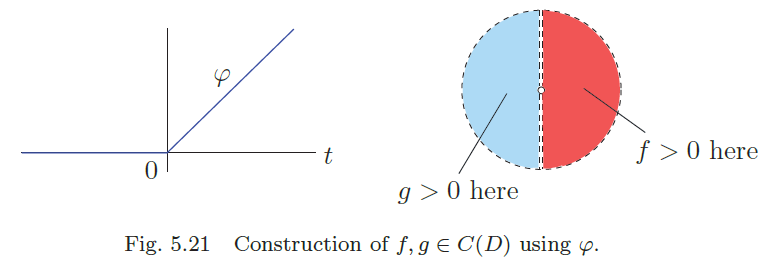
\includegraphics[width=0.8\textwidth]{./Solution/figs/fig-5-21}
\end{center}
\caption{$\varphi$를 이용한 연속함수 $f,g\in C(D)$의 구성
}
\label{fig-5-21}
\end{figure}

\subsection*{연습문제 \ref{ex-4-24}}

\begin{itemize}
\item[(1)]   거짓.
$D=\mathbb C$, $f=\exp$, $g=1$이라 하자.
그러면, 모든 $n\in \mathbb N$에 대하여
$f(2\pi i n) = \exp(2\pi i n) = 1 = g(2\pi i n)$이고,
$f\ne g$이다 (예를 들면, $f(i\pi) = -1 \ne 1 = g(i\pi)$).
\item[(2)] 참.
\item[(3)] 참. 
$\gamma(t) = x(t) +iy(t)$, $t\in[a,b]$라 하자.
$x'(t_0)$ 또는 $y'(t_0)$가 $0$이 아닌 점 $t_0$를 생각하자.
(이런 점이 없다면 두 값이 항상 $0$이므로 $a=b$가 되어 모순이다.)
$x'(t_0)>0$이라 가정하자. (다른 경우도 유사하게 다룰 수 있다.)
그러면, $t_0$의 근방에서 $x'(t)>0$이고 $x$가 증가한다.
$t_0+\dfrac1N\in [a,b]$가 되도록 충분히 큰 $N$을 잡고 $t_n = t_0 + \dfrac1n$, $n\ge N$라 하면,
$z_n(t_n)$으로 정의된 수열 $(z_n)_{n\ge N}$은 $\gamma(t_0)$로 수렴하는
서로 다른 점들로 구성된 수열이다. (적어도 실수부가 서로 다른 값을 갖는다.)
따라서 항등정리에 의하여 $D$에서 $f=g$이다.
\item[(4)] 참. 
테일러 정리를 적용하면 $w$를 중심으로 하는 원판에서 $ f=g$임을 알 수 있고,
여기에 항등정리를 쓰면, $D$에서 $f=g$를 얻는다.
\end{itemize}

\subsection*{연습문제 \ref{ex-4-25}}

$K=\{z\in\mathbb C\,:\, |z|\le 1\}$이라 하자.
$z\in K$에 대하여, $z$ 근방의 $w$에 대하여
\[
f(w) = \sum_{n=0}^\infty c_n(z)(w-z)^n
\]
로 나타낼 때, $c_{n(z)}(z)=0$인 가장 작은 $n(z)\in\{0,1,2,3,\ldots\}$이 존재한다.
따라서 $(f^{(n(z))}(z))/((n(z))!)=0$이므로 $f^{(n(z))}(0)=0$이다.
$\varphi:K\to \mathbb N \cup \{0\}$를 $\varphi(z)=n(z)$로 정의하자.
$K$가 비가산(uncountable) 집합이고, $\mathbb N\cup \{0\}$은 가산(countable) 집합이므로,
$\varphi^{-1}(N)$이 무한이 되는 $N$이 존재한다.
$(z_n)_{n\in\mathbb N}$을 $\varphi^{-1}(N)$의 서로 다른 점으로 만든 수열이라 하자.
$K$가 콤팩트 집합\footnote{
역주: 실수 $\mathbb R$ 또는 복소수  $\mathbb C$에서
콤팩트 집합(compact set)은 유계인 닫힌집합(closed and bounded set)을 뜻한다.
}이므로, $K$의 한점 $z_*\in K$로 수렴하는 부분수열 $(z_{n_k})_{k\in\mathbb N}$을
택할 수 있다\footnote{
역주: 볼자노-바이어스트라스 정리(Bolzano-Weierstrass theorem)에 의하여
콤팩트 집합 $K$에 정의한 수열 $(z_n)$은 $K$의 어떤 점 $z_*$으로 수렴하는
부분 수열을 갖는다. 
}. 
모든 $k$에서 $f^{(N)}(z_{n_k})=0$이므로  함수 $f^{(N)}$에 대하여 항등정리를 적용하면
$K$에서 $f^{(N)}=0$이다. 따라서 $\mathbb C$에서도  항등적으로 $0$이다.
테일러 정리에 의해, 모든 $z\in\mathbb C$에 대하여
\[
f(z) = \sum_{n=0}^\infty \dfrac{f^{(n)}(0)}{n!} z^n= \sum_{n=0}^{N-1} \dfrac{f^{(n)}(0)}{n!}z^n
\]
이므로 $f$는 다항식이다.

\subsection*{연습문제 \ref{ex-4-26}}

모든 $z\in D$에 대하여 $|f(z_0)| \ge |f(z)|$를 만족하는 점을 $z_0\in D$라 하자.
최대절대값정리에 의하여 $f$는 $D$에서 상수함수가 되어 모순이다.

\subsection*{연습문제 \ref{ex-4-27}}

$f(z_0)\ne0$라고 하자.
그러면 $|f(z_0)|>0$이고,
모든 $z\in D$에 대하여 $|f(z)|\ge|f(z_0)|>0$이므로
모든 $z\in D$에 대하여 $f(z)\ne0$이다.
이제 $D$에 정의된 복소해석함수 $g:=1/f$를 생각하면,
\[
|g(z_0)|  = \dfrac1{|f(z_0)|} \ge \dfrac1{|f(z)|} = |g(z)|,
\quad z\in D
\]
이고 최대절대값정리를 쓰면 $g$는 상수함수이다. 따라서 $f$도 상수함수이다.

\subsection*{연습문제 \ref{ex-4-28}}

$z\mapsto |f(z)|$가 연속함수이고, $K:=\{z\in \mathbb C\,:\, |z|\le 1\}$가
콤팩트 집합이므로 최대가 되는 점 $z_0$가 존재한다.
그런데 $z_0$는 $K$의 내점(interior point)될 수는 없다.
실제로 $|z_0|<1$이라면, 
$\mathbb D:=\{z\in \mathbb C\,:\, |z|<1\}$에 정의된 $f$에
최대절대값정리를 적용하여 $f$는 $\mathbb D$에서 상수함수가 된다.
물론 이는 모순이고 $z_0\in \mathbb T:=\{z\in \mathbb C\,:\, |z|= 1\}$이 되어야 한다.
따라서,
\[
\max_{z\in K} |f(z)| = \max_{|z|=1}|f(z)|
= \max_{t\in[0,2\pi)} |\exp(2it)-2| = |-1-2| = 3.
\]
같은 방법으로, 최소가 되는 점 $z_1$도 $K$의 내점이 될 수 없다.
$z_1^2-2\ne 0$이므로 최소절대값정리를 쓰면 $f$는 상수함수가 되어 모순이다.
따라서 $z_1\in\mathbb T$도 성립한다. 
\[
\min_{z\in K} |f(z)| = \min_{|z|=1}|f(z)|
= \min_{t\in[0,2\pi)} |\exp(2it)-2| = |1-2| = 1.
\]
그림 \ref{fig-5-22}\를 참고하라.

\begin{figure}[h!]
\begin{center}
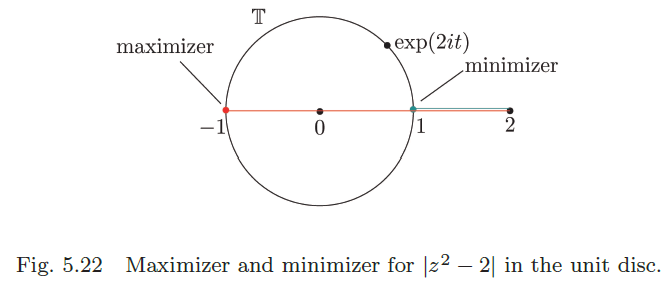
\includegraphics[width=0.4\textwidth]{./Solution/figs/fig-5-22}
\end{center}
\caption{단위원에서 $|z^2-2|$를 최대로 하는 점과 최소로 하는 점
}
\label{fig-5-22}
\end{figure}

\subsection*{연습문제 \ref{ex-4-29}}

$z\in \mathbb A_1 := \{ z\in\mathbb C\,:\, 0<|z-1|<1\}$에 대하여
\begin{align*}
\dfrac1{z(z-1)}
&= \dfrac1{(z-1+1)(z-1)} \\
&= \dfrac1{z-1}\Big(1-(z-1) + (z-1)^2 - (z-1)^3 + \cdots\Big) \\
&= \dfrac1{z-1} - 1 + (z-1) - (z-1)^2 + (z-1)^3 - \cdots.
\end{align*}

한편
$z\in \tilde {\mathbb A_1} := \{ z\in\mathbb C\,:\, 1<|z-1|\}$에 대하여
\begin{align*}
\dfrac1{z(z-1)}
&= \dfrac1{(z-1+1)(z-1)}
= \dfrac1{(z-1)^2\left( 1+ \dfrac1{z-1}\right)} \\
&= \dfrac1{(z-1)^2}\left( 1- \dfrac1{z-1} + \dfrac1{(z-1)^2} - \dfrac1{(z-1)^3} + \cdots \right) \\
&= \dfrac1{(z-1)^2} - \dfrac1{(z-1)^3} + \dfrac1{(z-1)^4} - \dfrac1{(z-1)^5} + \cdots.
\end{align*}

\subsection*{연습문제 \ref{ex-4-30}}

근의 분류 정리로부터 $z\in D$에서
$f(z) = (z-z_0)^mg(z)$이고 $g$는 복소해석함수로 $g(z_0)\ne0$이다.
$D$에서 $z_0$는 $f$의 유일한 근이므로, $D$에서 $g(z)\ne0$이다.
따라서 $1/g$가 복소해석함수이고 $z_0$를 중심으로 하는 원판에서 테일러 급수 전개가 가능하다.
즉, 상수 $R>0$이 존재하여
\[
\dfrac1{g(z)} = \sum_{n=0}^\infty c_n(z-z_0)^n,
\quad |z-z_0|<R
\]
이고 $c_0\ne0$이다 ($g(z_0)\ne0$이므로). 
$0<|z-z_0|<R$에 대하여,
\begin{align*}
\dfrac1{f(z)} 
&= \dfrac1{(z-z_0)^m g(z)} = \dfrac1{(z-z_0)^m} \sum_{n=0}^\infty c_n(z-z_0)^n \\
&= \dfrac{c_0}{(z-z_0)^m} +  \dfrac{c_1}{(z-z_0)^{m-1}} + \cdots 
+  \dfrac{c_{m-1}}{z-z_0} + \sum_{n=0}^\infty c_{m+n} (z-z_0)^n.
\end{align*}
따라서 $1/f$는 $z_0$에서 $m$ 중극을 갖는다.

\subsection*{연습문제 \ref{ex-4-31}}

$z\mapsto (z-z_0)^m f(z)$는 $D$에서 복소해석함수 $h$로 확장될 수 있다.
또한, 
\[
\neg\left( \lim_{z\to z_0} (z-z_0)^m f(z) = 0 \right)
\]
이므로 $h(z_0) \ne 0$이다. 
$z\in D$에서 $f(z)\ne0$이므로, 모든 $z\in D$에 대하여 $h(z)\ne0$이다.
따라서
\[
\dfrac1{f(z)} = \dfrac{(z-z_0)^m}{h(z)},
\quad z\in D\setminus \{z_0\}
\]
이고 
\[
g(z):= \dfrac{(z-z_0)^m}{h(z)},
\quad z\in D
\]
로 정의하면 $g$는 $D$에서 복소해석함수이다.
$\dfrac1{h(z_0)}\ne0$이므로 $z_0$는 $g$의 $m$ 중근이다.

\subsection*{연습문제 \ref{ex-4-32}}

모든 $n<-m$에 대하여 $c_n=0$이므로
\[
f(z) = \dfrac{c_{-m}}{(z-z_0)^m} + \dfrac{c_{-m+1}}{(z-z_0)^{m-1}}
+ \cdots + \dfrac{c_{-1}}{z-z_0} + \sum_{n=0}^\infty c_n(z-z_0)^n.
\]
따라서 $(z-z_0)^m f(z) = c_{-m} + c_{-m+1}(z-z_0) + \cdots + c_{-1}(z-z_0)^{m-1} + \cdots$는
\[
\Delta:= \{ z\in \mathbb C \,:\, |z-z_0|<R\}
\]
에서 복소해석함수 $g$로 확장가능하다.
$|z-z_0| <R$에서 
$g(z) = c_{-m} + c_{-m+1}(z-z_0) + \cdots + c_{-1}(z-z_0)^{m-1} + \cdots$의
테일러 정리를 적용하면,
\[
c_{-1} = \dfrac1{(m-1)!}\dfrac{d^{m-1}g}{dz^{m-1}}(z_0).
\]
한편, $g^{(m-1)}$은 $\Delta$에서 복소해석함수이며,
특히, $z_0$에서 연속이므로
\[
g^{(m-1)}(z_0) = \lim_{z\to z_0} g^{(m-1)}(z).
\]
또한, $0<|z-z_0|<R$에서 $g(z) = (z-z_0)^m f(z)$이고
$\Delta$의 점 $z\ne z_0$에서
\[
g^{(m-1)}(z) = \dfrac{d^{m-1}}{dz^{m-1}}((z-z_0)^m f(z)).
\]
따라서
\begin{align*}
c_{-1} &= \dfrac1{(m-1)!} g^{(m-1)}(z_0) 
= \dfrac1{(m-1)!} \lim_{z\to z_0} g^{(m-1)}(z) \\
&= \dfrac1{(m-1)!} \lim_{z\to z_0} \dfrac{d^{m-1}}{dz^{m-1}}((z-z_0)^m f(z)).
\end{align*}

\subsection*{연습문제 \ref{ex-4-33}}

\begin{itemize}
\item[(1)] 참. 
$c_{-1}=1\ne0$이고 $c_{-2} = c_{-3} = \cdots = 0$.
\item[(2)] 참.
\item[(3)] 참.
\item[(4)] 참.
\item[(5)] 참.
\end{itemize}

\subsection*{연습문제 \ref{ex-4-34}}

\begin{itemize}
\item[(1)]  $\sin z$는 $0$을 특이점으로 갖지 않는다.
$z\in \mathbb C$에 대하여
\[
\sin z = z - \dfrac{z^3}{3!} + \dfrac{z^5}{5!} - \cdots.
\]
\item[(2)] $\sin \dfrac1z$는 $0$을 본질적 특이점으로 갖는다. $z\ne0$에 대하여
\[
\sin \dfrac1z = \cdots + \dfrac1{5!z^5} - \dfrac1{3!z^3} + \dfrac1z.
\]
\item[(3)]  $\dfrac{\sin z}z$는 $0$에서 제거가능한 특이점을 갖는다.
\[
\lim_{z\to 0} z\cdot \dfrac{\sin z}z = \lim_{z\to 0} \sin z = 0.
\]
따라서 $\dfrac{\sin z}{z} = 1  - \dfrac1{3!}z^2  + \dfrac1{5!}z^4 - \dfrac1{7!}z^6 + \cdots$
($z\ne0$).
\item[(4)] $\dfrac{\sin z}{z^2}$은 $0$에서 $1$차의 극을 갖는다.
$z\ne0$에 대하여
\[
\dfrac{\sin z}{z^2} = \dfrac1z - \dfrac z{3!} + \dfrac{z^3}{5!} - \dfrac{z^5}{7!} + \cdots.
\]
\item[(5)] $1/(\sin(1/z))$는 $0$에서 고립 특이점을 갖지 않는다. 왜냐하면,
$z_n = 1/(n\pi)$, $n\in\mathbb N$에서 
\[
\sin \dfrac1{z_n} = \sin(n\pi) = 0
\]
이고 $z_n = \dfrac1{n\pi} \stackrel{n\to\infty}{\longrightarrow} 0$
이기 때문이다. (이러한 현상은 예제 \ref{example-4-13}에서와 같다.)
\item[(6)] $z\sin\dfrac1z$는 $0$을 본질적 특이점으로 갖는다.
$z\ne0$에 대하여
\[
z\sin \dfrac1z = \cdots + \dfrac1{5!z^4} - \dfrac1{3!z^2} +1.
\]
\end{itemize}

\subsection*{연습문제 \ref{ex-4-35}}

\begin{itemize}
\item[(1)] 거짓.
$\Lim_{z\nearrow 0} |e^{\frac1x}| = \Lim_{x\nearrow 0} e^{\frac1x} = 0$
이므로 $\neg \left( \lim_{z\to 0} \left| \exp\dfrac1z\right| = + \infty \right)$.
\item[(2)] 참.
$0<|z-z_0|<R$에 대하여
\[
f(z) = \dfrac{c_{-m}}{(z-z_0)^m} + \dfrac{c_{-m+1}}{(z-z_0)^{m-1}} + \cdots 
+ \dfrac{c_{-1}}{z-z_0} + \sum_{n=0}^\infty c_n(z-z_0)^n
\]
을 만족하는 $R>0$이 존재하므로
\[
p:= c_{-m} + c_{-m+1}(z-z_0) + \cdots  + c_{-1}(z-z_0)^{m-1}
\]
이라 하면, $0<|z-z_0|<R$에서
\[
f(z) - \dfrac{p(z)}{(z-z_0)^m} = \sum_{n=0}^\infty c_n(z-z_0)^n.
\]
\item[(3)] 참.
$0$이 $f$의 $m$중근이라고 하자 ($f(0)\ne0$인 경우 $m=0$이라 하자).
그러면 $f(z)=z^mg(z)$이고 $g(0)\ne0$인 복소해석함수 $g$가 존재한다.
$n>m$에 대하여, $z\ne0$이면
\[
\dfrac{f(z)}{z^n} = \dfrac{z^mg(z)}{z^n} = \dfrac{g(z)}{z^{n-m}}.
\]
따라서, $g(0)\ne0$이고 $n>m$이므로
\[
\lim_{z\to0} \left| \dfrac{f(z)}{z^n}\right| 
=\lim_{z\to0} \dfrac{|g(z)|}{|z|^{n-m}} = |g(0)|\cdot \lim_{z\to0}\dfrac1{|z|^{n-m}} = +\infty
\]
\item[(4)] 참.
뚫린원판 $D=\{ z\in \mathbb C\,:\, 0<|z-z_0| <R\}$에서
$f,g$가 $0$이 아니고 $h_f(z_0)\ne0$, $h_g(z_0)\ne0$인 복소해석함수 $h_f, h_g$가 존재하여
모든 $z\in D$에 대하여
\[
\dfrac1{f(z)} = (z-z_0)^{m_f} h_f(z),\quad
\dfrac1{g(z)} = (z-z_0)^{m_g} h_g(z).
\]
따라서 $h_f(z_0)h_g(z_0)\ne0$이고 모든 $z\in D$에 대하여
\[
\dfrac1{f(z)g(z)} = (z-z_0)^{m_f+m_g} h_f(z)h_g(z).
\]
결론적으로, $fg$는 $z_0$에서 $m_f+m_g$차 극을 갖는다.
\end{itemize}

\subsection*{연습문제 \ref{ex-4-36}}

\[
f(z) = \exp \left(\dfrac 1z \right) + \exp \left(\dfrac1{1-z}\right),
\quad z\in \mathbb C\setminus\{0,1\}
\]
은 $\mathbb C\setminus\{0,1\}$에서 복소해석함수이다.
함수 $\exp(1/(1-z))$는 $z=0$ 근방에서 복소해석함수이고
$\exp(1/z)$는 $0$을 본질적 특이점으로 갖는다. 따라서 그 합 $f$는 $0$을
본질적 특이점으로 갖는다. (왜?) 한편, $1$ 근방에서 $\exp(1/z)$는 복소해석함수이고
$\exp(1/(1-z))$는 본질적 특이점을 갖는다. 따라서 $f$도 $z=1$을 본질적 특이점으로 갖는다.

\subsection*{연습문제 \ref{ex-4-37}}

$z_0$가 $g$의 고립 특이점이면 
$0<|z-z_0|<R$에서 로랑급수 전개
\[
g(z) = \sum_{n\in\mathbb Z} c_n(z-z_0)^n
\]
를 주는 적당한 $R>0$이 존재한다.
$c_n\ne0$인  $n<0$이 무한이 많으면 $z_0$는 $g$의 본질적 특이점이다.

그런데 주어진 $f$는 $|z|>1$로 주어진 뚫린원판에서 로랑급수 전개
\[
z^{-1} + z^{-2} + z^{-3} + \cdots
\]
를 갖는다. 특이점 $0$의 특성을 규정하려면 
적당한 $R>0$에 대하여 $0<|z|<R$에서 함수를 살펴봐야 한다.
$|z|<1$에서 
\[
f(z) = - \dfrac1{1-z} = - (1+z+z^2+ z^3 + \cdots )
\]
이므로 $ |z|<1$에서 $f$는 복소해석함수이고
$z=0$에서 특이점을 갖지 않는다.

\subsection*{연습문제 \ref{ex-4-38}}

$z_0$가 $fg$의 고립 특이점임은 분명하다.
$f$와 $g$가 $z_0$에서 고립 특이점을 갖기 때문에
뚫린원판 $0<|z-z_0|<R_f$에서 $f$가 복소해석함수인  $R_f>0$가 존재하고
뚫린원판 $0<|z-z_0|<R_g$에서 $g$가 복소해석함수인  $R_g>0$가 존재한다.
따라서 뚫린원판  $0<|z-z_0| < \min\{R_f, R_g\}$에서
$fg$는 복소해석함수이다.

$z_0$가 $fg$의 제거가능한 특이점이거나 극이라고 가정하자.
그러면, 적당한 $m>1$이 존재하여
\[
\lim_{z\to z_0} (z-z_0)^m f(z)g(z) = 0
\]
을 만족한다.
$f$가 $z_0$에서 극을 가지므로, $m_f$중극을 갖는다고 하면,
$f$는 $z_0$ 근방에서 $0$이 아니며, $0<|z-z_0|<R$에서
\[
f(z) = \dfrac{c_{-m_f}}{(z-z_0)^{m_f}} + \dfrac{c_{-m_f+1}}{(z-z_0)^{m_f-1}} +
\cdots + \dfrac{c_{-1}}{z-z_0} + \sum_{n=0}^\infty c_n(z-z_0)^n
\]
을 만족하는 $R>$이 존재한다.
여기서 $c _{m_f} \ne0$이다.
따라서 $z\ne z_0$인 $z_0$ 근방에서
\begin{align*}
(z-z_0)^mg(z)
&= \dfrac1{(z-z_0)^{m_f}f(z)} \cdot \underbrace{(z-z_0)^{m_f}}_{\to0}
\underbrace{(z-z_0)^mf(z)g(z)}_{\to 0} \\
&\stackrel{z\to z_0}{\longrightarrow} \dfrac1{c_{-m_f}}\cdot 0 \cdot 0 - 0.
\end{align*}
그렇다면 $g$는 $z_0$에서 극을 갖거나 제거가능한 특이점을 갖게 되고
가정에 모순이 되므로 $fg$는 $z_0$에서 본질적 특이점을 갖는다.

\subsection*{연습문제 \ref{ex-4-39}}

$\epsilon:= 1/n =:\delta(>0)$으로 설정하자.
카소라티-바이어스트라스 정리에 의해
$z_0$를 중심으로 반지름 $\delta$인 뚫린원판에 점 $z_n$이 존재하여
$|f(z_n)-w|<\epsilon$을 만족한다.
즉, $|z_n - z_0| <1/n$이고 $|f(z_n) - w|< 1/n$.
따라서 $(z_n)_{n\in\mathbb N}$은 $z_0$로 수렴하고
$(f(z_n))_{n\in\mathbb N}$은 $w$로 수렴한다.

\subsection*{연습문제 \ref{ex-4-40}}

$1+\exp z =0$일 필요충분조건은 $ z\in \{ \pi i +2\pi n i \,:\, n\in \mathbb Z\}$이다.
따라서
\[
f(z):= \dfrac{Log(z)}{1+\exp z}
\]
는 $(\mathbb C\setminus(-\infty,0])\setminus \{ \pi i +2\pi n i \,:\, n\in \mathbb Z\}$에서
복소해석함수이다.
$f$는 $\{ \pi i +2\pi n i \,:\, n\in \mathbb Z\}$에 속하는 점에서 $1$차의 극을 가진다.
경로 $\gamma$의 내부에는 $-\pi i$와  $3\pi i$가 속한다. 그림 \ref{fig-5-23}\을 참고하라.

\begin{figure}[h!]
\begin{center}
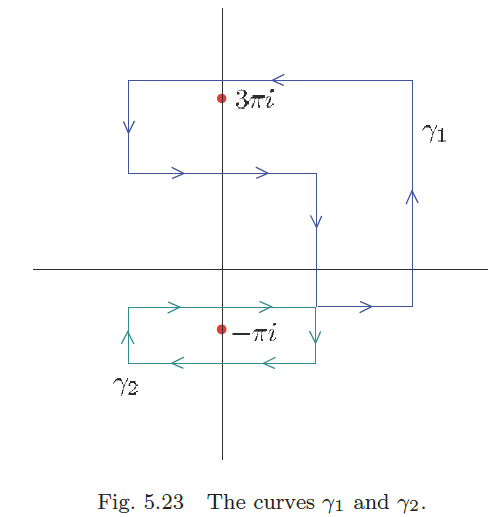
\includegraphics[width=0.4\textwidth]{./Solution/figs/fig-5-23}
\end{center}
\caption{경로 $\gamma_1$과 $\gamma_2$
}
\label{fig-5-23}
\end{figure}

\[
\int_\gamma f(z) dz = \int_{\gamma_1} f(z) dz + \int_{\gamma_2} f(z) dz
= 2\pi i (\res(f,3\pi i) - \res(f, -\pi i))
\]
이므로 $\res(f, 3\pi i)$와 $\res(f, \pi i)$를 계산해야 한다.
\[
\dfrac{\Log(z)}{1+\exp z} = \dfrac{c_{-1,3\pi i}}{z-3\pi i} + h_{3\pi i}
\]
로 쓸 수 있다. 여기서, $h_{3\pi i}$는 $3\pi i$ 근방에서 복소해석함수이다.
따라서
\begin{align*}
c_{-1,3\pi i}
&= \lim_{z\to 3\pi i} \dfrac{(z-3\pi i)\Log(z)}{1+\exp z} 
= \lim_{z\to 3\pi i} \dfrac{z-3\pi i}{\exp z - \exp(3\pi i)}\cdot \Log(z) \\
&= \dfrac1{\exp z|_{z=3\pi i}} \cdot \Log(3\pi i) = -1\left( \log|3\pi i| + i\dfrac\pi2 \right) \\
&= - \log 3 - \log\pi- i\dfrac\pi2.
\end{align*}
한편,
\[
\dfrac{\Log(z)}{1+\exp z} = \dfrac{c_{-1,-\pi i}}{z-(-\pi i)} + h_{-\pi i}
\]
로 쓸 수 있다. 여기서, $h_{-\pi i}$는 $-\pi i$ 근방에서 복소해석함수이다.
따라서
\begin{align*}
c_{-1,-\pi i}
&= \lim_{z\to -\pi i} \dfrac{(z-(-\pi i))\Log(z)}{1+\exp z} 
= \lim_{z\to -\pi i} \dfrac{z-(-\pi i)}{\exp z - \exp(-\pi i)}\cdot \Log(z) \\
&= \dfrac1{\exp z|_{z=-\pi i}} \cdot \Log(-\pi i) 
= -1\left( \log|-\pi i| + i\left(-\dfrac\pi2 \right)\right) \\
&= - \log\pi +  i\dfrac\pi2.
\end{align*}

종합하면,
\[
\int_\gamma \dfrac{\Log(z)}{1+\exp z} dz
= 2\pi i \left( -\log 3 - \log \pi - i\dfrac\pi2 + \log \pi - i\dfrac\pi 2\right)
= 2\pi^2 - (2\pi \log 3)i.
\]

\subsection*{연습문제 \ref{ex-4-41}}

$\gamma(\theta)  = \exp(i\theta)$, $\theta\in [0,2\pi)$의
원형경로로 적분경로 $\gamma$를 정의하자.
그러면,
\begin{align*}
\int_0^{2\pi} \dfrac{\cos\theta}{5+4\cos\theta} d\theta
&= \int_\gamma \dfrac{\dfrac{z+\frac1z}2}{5+4\dfrac{z+\frac1z}2}\cdot \dfrac1{iz}dz
= \int_\gamma \dfrac{z^2+1}{2iz(2z^2+5z+1)}dz \\
&= \int_\gamma \dfrac{z^2+1}{2iz(2z+1)(z+3)}dz.
\end{align*}
\[
f(z):= \dfrac{z^2+1}{2iz(2z+1)(z+3)}
\]
라 정의하면, $f$는 $0$, $-1/2$, $-2$에서 $1$차의 극을 갖는다.
경로 $\gamma$의 내부에는 $0$과 $-1/2$이 있으므로
유수정리를 쓰면,
\begin{align*}
\int_0^{2\pi} & \dfrac{\cos\theta}{5+4\cos\theta} d\theta \\
&=2\pi i \left(\res(f,0) + \res(f,-1/2)\right) \\
&=2\pi i \left(\lim_{z\to0} \dfrac{z\cdot(z^2+1)}{2iz(2z+1)(z+3)}
+ \lim_{z\to1/2} \dfrac{(z+1/2)\cdot(z^2+1)}{2iz(2z+1)(z+3)} \right) \\
&= 2\pi i \left( \dfrac1{2i\cdot 1\cdot 2} 
+ \dfrac{1\cdot\frac54}{2i\cdot (-\frac12)\cdot2\cdot\frac32} \right)
= 2\pi i \left( \dfrac1{4i} - \dfrac4{12i} \right) \\
&= -\dfrac\pi3.
\end{align*}

\subsection*{연습문제 \ref{ex-4-42}}

\begin{itemize}
\item[(1)] $f_1$을 다음과 같이 정의하자.
\[
f_1(z) = \dfrac1{1+z^2}.
\]
그러면 $f_1$은 $i$와 $-i$에서 $1$차 극을 갖는다. 따라서
\begin{align*}
\int_0^\infty \dfrac1{1+x^2}dx &= \dfrac12 \cdot2\pi i \cdot \res(f_1, i)
= \pi i \cdot \lim_{z\to i} \dfrac{z-i}{1+z^2} \\
&= \pi i \cdot \lim_{z\to i} \dfrac1{z+i} = \pi i \cdot \dfrac1{2i} = \dfrac\pi 2.
\end{align*}
\item[(2)] $f_2$를 다음과 같이 정의하자.
\[
f_2(z) = \dfrac1{(a^2+z^2)(b^2+z^2)}.
\]
그러면 $f_2$는 $ai$, $-ai$, $bi$, $-bi$에서 $1$차 극을 갖는다. 
$f_2$가 우함수이므로
\begin{align*}
\int_0^\infty \dfrac1{(a^2+x^2)(b^2+x^2)}dx
&= \dfrac12 \cdot 2\pi i \left( \res(f_2, ai) + \res(f_2, bi) \right) \\
&= \pi i \left( \dfrac1{(b^2-a^2)2ai} + \dfrac1{(a^2-b^2)2bi} \right) \\
&= \dfrac\pi{2(a^2-b^2)} \left( \dfrac1b-\dfrac1a\right) = \dfrac\pi{2ab(a+b)}.
\end{align*}
\item[(3)]  $f_3$를 다음과 같이 정의하자.
\[
f_3(z) = \dfrac1{(1+z^2)^2}.
\]
그러면 $f_3$는 $i$, $-i$에서 $2$차 극을 갖는다. 
\begin{align*}
\int_0^\infty \dfrac1{(1+x^2)^2}dx
&= \dfrac12 \cdot 2\pi i \cdot \res(f_3, i) \\
&= \dfrac\pi{1!}\cdot \lim_{z\to i} \dfrac d{dz} \left(
(z-i)^2 \cdot \dfrac1{(z-i)^2(z+i)^2} \right) \\
&= \pi i \cdot \lim_{z\to i} \dfrac{-2}{(z+i)^3} = \pi i \cdot \dfrac{-2}{-8i}
= \dfrac\pi4.
\end{align*}
\item[(4)] $f_4$를 다음과 같이 정의하자.
\[
f_4(z) = \dfrac{1+z^2}{1+z^4}.
\]
그러면 $f_4$는 다음 점들에서 $1$차 극을 갖는다. 
\[
p_1 =\exp\left(\dfrac{\pi i }4\right), \quad
p_2 =\exp\left(\dfrac{3\pi i }4\right), \quad
p_3 =\exp\left(\dfrac{5\pi i }4\right), \quad
p_4 =\exp\left(\dfrac{7\pi i }4\right).
\]
\begin{align*}
\int_0^\infty \dfrac{1+x^2}{1=x^4}dx 
&= \dfrac12\cdot 2\pi  i\left(\res(f_4,p_1) + \res(f_4,p_2) \right)
=\pi i \left( \dfrac{1+p_1^2}{4p_1^3} + \dfrac{1+p_2^2}{4p_2^3} \right) \\
&= \pi i \left( \dfrac{p_1}{4p_1^4} + \dfrac1{4p_1} + \dfrac{p_2}{4p_2^4} + \dfrac1{4p_2} \right)
= \pi i \left( - \dfrac{p_1+p_2}{4} + \dfrac1{4p_1} + \dfrac1{4p_2} \right) \\
&= \pi i \left( - \dfrac{\exp(i\pi/4) - \exp(-\pi i/4)}4 
+ \dfrac{\exp(-i\pi/4) - \exp(i\pi/4)}4 \right) \\
&= \pi i \left( - \dfrac{i\sin(\pi/4)}2 + \dfrac{-i\sin(\pi/4)}2 \right)
= \pi i \cdot(-1) \cdot \dfrac1{\sqrt{2}} = \dfrac\pi{\sqrt{2}}.
\end{align*}
\end{itemize}
 
\subsection*{연습문제 \ref{ex-4-43}}

유수정리를 이용하면,
\begin{align*}
\int_C \dfrac{\exp z}{z^{n+1}} dz
&= 2\pi i \cdot \res\left(\dfrac{\exp z}{z^{n+1}}, 0\right) 
= \dfrac{2\pi i}{n!} \cdot \lim_{z\to 0} \dfrac{d^n}{dz^n} 
\left(z^{n+1}\cdot \dfrac{\exp z}{z^{n+1}} \right) \\
&= \dfrac{2\pi i}{n!} \cdot \lim_{z\to 0} \dfrac{d^n}{dz^n} \exp z
= \dfrac{2\pi i}{n!} \cdot \lim_{z\to 0} \exp z 
= \dfrac{2\pi i}{n!} \cdot \exp 0 \\
&= \dfrac{2\pi i}{n!} \cdot 1 =  \dfrac{2\pi i}{n!}.
\end{align*}
따라서,
\begin{align*}
\dfrac{2\pi i}{n!}
&= \int_0^{2\pi} \dfrac{\exp(\cos\theta + i \sin\theta)}
{cos((n+1)\theta) + i\sin((n+1)\theta)} \cdot
i(\cos\theta + i\sin\theta) d\theta \\
&= i\int_0^{2\pi} \exp(\cos\theta + i\sin\theta)\cdot
\left(\cos(n\theta) - i\sin(n\theta) \right) d\theta \\
&=i\int_0^{2\pi} \exp(\cos\theta)\left(\cos(n\theta-\sin\theta)
- i \sin(n\theta - \sin\theta)\right)d\theta.
\end{align*}
양변의 허수부를 비교하여
\[
\int_0^{2\pi} \exp(\cos\theta)\cdot \cos(n\theta-\sin\theta) d\theta
= \dfrac{2\pi}{n!}.
\]
 
\subsection*{연습문제 \ref{ex-4-44}}

중심이 $z_0$인 작은 뚫린원판 $D$에서 $f(z)\ne0$이고
\begin{equation}\label{eq-5-26}
f(z) = (z-z_0)h(z)
\end{equation}
를 만족하는 $h(z_0)\ne0$인 복소해석함수 $h$가 존재한다.
식 \eqref{eq-5-26}에 의해
$f'(z) = h(z) + (z-z_0)h'(z)$로 쓸 수 있다.
특히, $f'(z_0) = h(z_0)$이다.
$z\in D\setminus \{z_0\}$에 대하여
\[
\dfrac1{f(z)} = \dfrac1{(z-z_0)h(z)}
\]
이고 $\dfrac1h$이 $D$에서 복소해석함수이므로
\[
\dfrac1{h(z)} = d_0 + d_1(z-z_0) + \cdots
\]
이고 $d_0 = \dfrac1{h(z_0)} = \dfrac1{f'(z_0)}$이다.
따라서 $z\in D\setminus\{z_0\}$에 대하여
\[
\dfrac1{f(z_0)} = \dfrac1{z-z_0} \cdot(d_0 + d_1(z-z_0) + \cdots)
= \dfrac{d_0}{z-z_0} + d_1 + d_2(z-z_0) + \cdots
\]
이고 $\res\left( \dfrac1f, z_0\right) = d_0 = \dfrac1{f'(z_0)}$.

\subsection*{연습문제 \ref{ex-4-45}}

$f(z) = \sin z$라고 하자.
$f$는 $k\pi$, $k\in\mathbb Z$에서 $1$차의 근을 갖는다.
앞의 연습문제에 의하여
\[
\res\left(\dfrac1{\sin z}, k\pi \right)
= \dfrac1{\sin' z|_{z=k\pi}} = \dfrac1{\cos(k\pi)}
= \dfrac1{(-1)^k} = (-1)^k.
\]

\subsection*{연습문제 \ref{ex-4-46}}

\begin{itemize}
\item[(1)]  $f_0=1\le 2^0=1$, $f_1 = 1\le 2^1=2$이고,
어떤 $n\ge1$이 존재하여 모든 $m\le n$에 대하여
$f_m\le 2^m$이 성립한다고 가정하면,
\[
f_{m+1} = f_m + f_{m-1} \le 2^m + 2^{m-1}
= 2^{m-1} \cdot3 < 2^{m-1}\cdot 4 = 2^{m+1}.
\]

\item[(2)] $|z|<1/2$이면, 모든 $n\in \mathbb N$에 대하여
$\sqrt[n]{|c_nz^n|} = \sqrt[n]{|c_n|}\cdot|z| \le \sqrt[n]{2^n}\cdot|z| = 2|z| < 1$.
근판정법에 의해
\[
\sum_{n=0}^\infty |c_nz^n|
\]
은 $|z|<1/2$일 때 수렴한다. 따라서 $F$의 수렴 반지름은 $1/2$보다 크거나 같다.

\item[(3)] $|z|<1/2$에 대하여
\begin{align*}
zF(z) &= f_0z + f_1z^2 + f_2z^3 + \cdots, \\
z^2F(z) &= \phantom{f_0z+\ }\, f_0z^2 + f_1z^3 + \cdots.
\end{align*}
두 식을 더하면,
\begin{align*}
zF(z) + z^2F(z) &= 1\cdot z + (f_1+z_0)z^2 + (f_2+f_1)z^3 + \cdots\\
&= f_1z + f_2z^2 + f_3z^3 + \cdots \\
&= (f_0 +  f_1z + f_2z^2 + f_3z^3 + \cdots ) - f_0 \\
&= F(z) =1.
\end{align*}
따라서
\[
1 = F(z) - zF(z) -z^2F(z) = (1-z-z^2)F(z)
\]
이고
$|z|<\dfrac12$에서 $F(z) = \dfrac1{1-z-z^2}$.

\item[(4)] 
\begin{align}
\dfrac1{z^{n+1}(1-z-z^2)}
&= \dfrac{F(z)}{z^{n+1}} \nonumber \\ 
&= \dfrac{f_0+\cdots + f_{n-1}z^{n-1} + f_nz^n + f_{n+1}z^{n+1} + \cdots}{z^{n+1}} \nonumber \\
&= \dfrac{f_0}{z^{n+1}} + \dfrac{f_1}{z^n} + \cdots + \dfrac{f_n}{z} + f_{n+1} + f_{n+2}z + \cdots
\label{eq-5-27}
\end{align}
이므로  유수를 계산하면
\[
\res\left( \dfrac1{z^{n+1}(1-z-z^2)}, 0\right)
= f_n. \ (\text{식 \eqref{eq-5-27}의 $\dfrac1z$의 계수})
\]

\item[(5)] $|z|=R>2$에 대하여
\begin{align*}
|1-z-z^2| &\ge |z^2+z| -1 = |z|\cdot|z+1| -1 = R\cdot |z+1| -1 \\
&\ge R\cdot(|z|-1)-1 = R\cdot(R-1) -1 = R^2 -R -1 \\
&>0 \ \text{($R>2$이므로)}.
\end{align*}
$C_R:[0,2\pi] \to \mathbb C$가 다음과 같은 원형경로이면,
\[
C_R(t) = R\exp(it), \quad t\in[0,2\pi],
\]
\begin{align*}
\left| \int_{C_R} \dfrac1{z^{n+1}(1-z-z^2)} dz \right|
&\le \dfrac1{R^{n+1}}\cdot\dfrac1{R^2-R-1}\cdot 2\pi R\\
&= \dfrac1{R^n}\cdot\dfrac1{R^2-R-1}
\stackrel{R\to\infty}{\longrightarrow} 0.
\end{align*}
$G(z):= \dfrac1{z^{n+1}(1-z-z^2)} $라 정의하면, $G$는
\begin{itemize}
\item[(a)] $0$에서 $n+1$차 극을 갖는다.
\item[(b)] $\dfrac{-1+\sqrt{5}}2$에서 $1$차 극을 갖는다.
\item[(c)] $\dfrac{-1-\sqrt{5}}2$에서 $1$차 극을 갖는다.
\end{itemize}
따라서 $R>2$에 대하여,
\[
\res(G,0) + \res\left(G, \dfrac{-1+\sqrt{5}}2\right)
+ \res\left(G, \dfrac{-1-\sqrt{5}}2\right) 
= \dfrac1{2\pi i} \int_{C_R} G(z) dz.
\]
\begin{align*}
\res(G,0) &+ \res\left(G, \dfrac{-1+\sqrt{5}}2\right)
+ \res\left(G, \dfrac{-1-\sqrt{5}}2\right) \\
&=  \lim_{R\to\infty} \dfrac1{2\pi i} \int_{C_R} G(z) dz = 0
\end{align*}
이므로,
\[
f_n = -\res\left(G, \dfrac{-1+\sqrt{5}}2\right)
- \res\left(G, \dfrac{-1-\sqrt{5}}2\right).
\]
\begin{align*}
\res\left(G, \dfrac{-1+\sqrt{5}}2\right)
&= \lim_{z\to \frac{-1+\sqrt{5}}2} \left( z - \dfrac{-1+\sqrt{5}}2 \right)
\cdot \dfrac1{z^{n+1}(1-z-z^2)} \\
&= \dfrac1{\left(\dfrac{-1+\sqrt{5}}2\right)^{n+1} \cdot(-\sqrt{5})} \\
&= \left(\dfrac{1+\sqrt{5}}2\right)^{n+1} \left(- \dfrac1{\sqrt{5}} \right).
\end{align*}
\[
\res\left(G, \dfrac{-1-\sqrt{5}}2\right)
= \dfrac1{\left(\dfrac{-1-\sqrt{5}}2\right)^{n+1} \cdot(-\sqrt{5})} 
= \left(\dfrac{1-\sqrt{5}}2\right)^{n+1} \left( \dfrac1{\sqrt{5}} \right).
\]
이를 종합하면,
\begin{align*}
f_n &= \dfrac1{\sqrt{5}} \cdot \left(\dfrac{1+\sqrt{5}}2\right)^{n+1}
- \dfrac1{\sqrt{5}} \cdot \left(\dfrac{1-\sqrt{5}}2\right)^{n+1} \\
&= \dfrac1{\sqrt{5}} \cdot \left( \left(\dfrac{1+\sqrt{5}}2\right)^{n+1}
- \left(\dfrac{1-\sqrt{5}}2\right)^{n+1} \right).
\end{align*}



\end{itemize}














%===[salt] 5장
% !TEX root = ../notes_template.tex

\section*{5장 - 연습문제 풀이}

\subsection*{연습문제 \ref{ex-5-1}}

\begin{itemize}
\item[(1)] $(x,y)\in \mathbb R^2\setminus\{(0,0)\}$에 대하여
\begin{align*}
\dfrac{\partial u}{\partial x} &= \dfrac1{x^2+y^2} \cdot 2x = \dfrac{2x}{x^2+y^2} \\
\dfrac{\partial^2 u}{\partial x^2} &= \dfrac2{x^2+y^2} - \dfrac{2x}{(x^2+y^2)^2} \cdot (2x) 
= \dfrac{2y^2+2x^2-4x^2}{(x^2+y^2)^2} = \dfrac{2(y^2-x^2)}{(x^2+y^2)^2}.
\end{align*}
$x$, $y$에 대한 대칭식임을 이용하면
\[
\dfrac{\partial u}{\partial y}  = \dfrac{2y}{x^2+y^2}, \quad
\dfrac{\partial^2 u}{\partial y^2} = \dfrac{2(x^2-y^2)}{(x^2+y^2)^2}.
\]
따라서,
\[
\dfrac{\partial^2 u}{\partial x^2} + \dfrac{\partial^2 u}{\partial y^2}
= \dfrac{2(y^2-x^2)}{(x^2+y^2)^2} + \dfrac{2(x^2-y^2)}{(x^2+y^2)^2} = 0.
\]
$\mathbb R^2\setminus\{(0,0)\}$에서
$u\in C^2$이고 $\Delta u=0$이므로, $u$는 조화함수이다.
\item[(2)] 
$(x,y) \in \mathbb R^2$에 대하여
\begin{align*}
\dfrac{\partial u}{\partial x} &= e^x\sin y, \ \dfrac{\partial^2 u}{\partial x^2} = e^x\sin y, \\
\dfrac{\partial u}{\partial y} &= e^x\cos y, \ \dfrac{\partial^2 u}{\partial y^2} = e^x(-\sin y).
\end{align*}
따라서, 
$\dfrac{\partial^2 u}{\partial x^2} + \dfrac{\partial^2 u}{\partial y^2}
= e^x\sin y + e^x(-\sin y) = 0$.
$\mathbb R^2$에서
$u\in C^2$이고 $\Delta u=0$이므로, $u$는 조화함수이다.
\end{itemize}

\subsection*{연습문제 \ref{ex-5-2}}

$U$에 정의된 실변수 함수의 점별 연산에 대한 공간 $V$를 생각하자.
$V$는 벡터공간이 됨을 알고 있다.
$\Har(U)$가 점별 연산에 대하여 $V$의 부분공간을 이룬다는 것을 증명하자.
\begin{itemize}
\item[(S1)]
$U$의 모든 점에서 $0$을 대응시키는 상수함수 $\bs 0$가 $\Har(U)$에 속한다.
\[
\dfrac{\partial^2 \bs 0}{\partial x^2} + \dfrac{\partial^2 \bs 0}{\partial y^2} = 0+0=0.
\]
\item[(S2)] $u,v\in \Har(U)$라고 하면,
\begin{align*}
\dfrac{\partial^2 (u+v)}{\partial x^2} + \dfrac{\partial^2 (u+v)}{\partial y^2}
&= \dfrac{\partial^2 u}{\partial x^2} + \dfrac{\partial^2 v}{\partial x^2}
+ \dfrac{\partial^2 u}{\partial y^2}+ \dfrac{\partial^2 v}{\partial y^2} \\ 
&= \left(\dfrac{\partial^2 u}{\partial x^2} + \dfrac{\partial^2 u}{\partial y^2} \right)
+ \left( \dfrac{\partial^2 v}{\partial x^2} + \dfrac{\partial^2 v}{\partial y^2} \right) \\
&= 0+0=0.
\end{align*}
\item[(S3)] $\alpha\in\mathbb R$이고, $u\in\Har(U)$이면,
\begin{align*}
\dfrac{\partial^2 (\alpha\cdot u)}{\partial x^2} + \dfrac{\partial^2 (\alpha\cdot u)}{\partial y^2}
&= \alpha\cdot \dfrac{\partial^2 u}{\partial x^2} 
+ \alpha \cdot \dfrac{\partial^2 u}{\partial y^2} \\
&= \alpha \left( \dfrac{\partial^2 u}{\partial x^2} + \dfrac{\partial^2 u}{\partial y^2} \right)
= \alpha\cdot 0 = 0.
\end{align*}
이상에서 $\Har(U)$는 점별 연산에 대하여 실 벡터공간이 된다.
\end{itemize}

\subsection*{연습문제 \ref{ex-5-3}}

$u:=x=\Re(z)$, $\tilde u:= x+y = \Re(z-iz)$는 모두 $\mathbb R^2$의
조화함수이다.
두 함수의 점별 곱은 $u\cdot \tilde u = x\cdot(x+y) = x^2 +xy$이다.
\[
\dfrac{\partial^2 (u\cdot \tilde u)}{\partial x^2} 
+ \dfrac{\partial^2 (u\cdot \tilde u)}{\partial y^2}
= \dfrac{\partial}{\partial x}(2x+y) + \dfrac{\partial}{\partial y}(x) = 2 + 0 = 2\ne 0.
\]
따라서 두 조화함수의 점별 곱이 반드시 조화함수가 되는 것은 아니다.

\subsection*{연습문제 \ref{ex-5-4}}

\begin{itemize}
\item[(1)] $u=e^x\sin y$라고 하자. $u+iv$가 복소해석함수인 $v$를 찾으면 된다.
코시-리만 방정식을 만족해야 하므로
\[
\dfrac{\partial v}{\partial x} = - \dfrac{\partial u}{\partial y}= -e^x\cos y.
\]
$y$를 고정하고 $x$로 적분하면 $v=-e^x \cos y + C(y)$를 얻는다. 
여기서 $C(y)$는 $y$에만 의존하는 적분상수이다.
\[
\dfrac{\partial v}{\partial  y} = e^x\sin y + C'(y) 
= \dfrac{\partial u}{\partial x} = e^x \sin y
\]
이므로 $C'(y)=0$에서 $C(y)=K$이다.
$v:= -e^x \cos y$로 두자. 그러면
\begin{align*}
u+iv &= e^x\sin y + i(-e^x\cos y) = e^x (\sin y - i\cos y) \\
&= -ie^x(\cos y +i\sin y) = -i \exp(x+iy) = -i\exp(z),
\end{align*}
여기서 $z=x+iy$이고
$u+iv = -i\exp z$는 실제로 복소해석함수이다.
따라서 $v:=-e^x\cos y$는 $u:=e^x\sin y$의 조화결레함수이다.

\item[(2)] $u= x^3_2xy^2-2y$라고 하자. $u+iv$가 복소해석함수인 $v$를 찾으면 된다.
코시-리만 방정식을 만족해야 하므로
\[
\dfrac{\partial v}{\partial x} = - \dfrac{\partial u}{\partial y}= 6xy+2.
\]
$y$를 고정하고 $x$로 적분하면 
\[
v = 6\dfrac{x^2}{2}y + 2x + C(y) = 3x^2y +2x+ C(y).
\]
여기서 $C(y)$는 $y$에만 의존하는 적분상수이다.
\[
\dfrac{\partial v}{\partial  y} = 3x^2 + C'(y) 
= \dfrac{\partial u}{\partial x} = 3x^2 - 3y^2
\]
이므로 $C'(y)=-3y^2$에서 
\[
 C(y) = -3\dfrac{y^3}{3} + C  = -y^3+C.
\]
$v:= 3x^2y+2x-y^3$으로 두자. 그러면
\begin{align*}
u+iv &= x^3-3xy^2 -2y +i(3x^2y + 2x-y^3) \\  
&= x^3 +3x(iy)^2 + 3x^2(iy) +(iy)^3 -2y +i2x \\
&= (x+iy)^3 + 2i(x+iy) = z^3+2iz.
\end{align*}
여기서 $z=x+iy$이고
$u+iv =z^3+2iz$는 실제로 복소해석함수이다.
따라서 $v:=3x^2y+2x-y^3$는 $u:=x^3_2xy^2-2y$의 조화결레함수이다.

\item[(3)] $u= x(1+2y)$라고 하자. $u+iv$가 복소해석함수인 $v$를 찾으면 된다.
코시-리만 방정식을 만족해야 하므로
\[
\dfrac{\partial v}{\partial x} = - \dfrac{\partial u}{\partial y}= -2x.
\]
$y$를 고정하고 $x$로 적분하면 
\[
v = 2\dfrac{x^2}{2} + C(y) = -x^2 + C(y).
\]
여기서 $C(y)$는 $y$에만 의존하는 적분상수이다.
\[
\dfrac{\partial v}{\partial  y} =  C'(y) 
= \dfrac{\partial u}{\partial x} = 1+2y
\]
이므로
\[
 C(y) = y + 2\cdot \dfrac{y^2}2 + C = y + y^2 + C.
\]
$v:= -x^2+y+y^2$으로 두자. 그러면
\begin{align*}
u+iv &= x(1+2y) + i(-x^2+y+y^2) = x+iy + 2xy + i(y^2-x^2) \\
&= x + iy -i( (x^2-y^ 2) +i2xy ) = x+ iy -i(x+iy)^2 \\
&=  z- iz^2.
\end{align*}
여기서 $z=x+iy$이고
$u+iv =z-iz^2$는 실제로 복소해석함수이다.
따라서 $v:=-x^2 + y+y^2$는 $u:=x(1+2y)$의 조화결레함수이다.

\end{itemize}

\subsection*{연습문제 \ref{ex-5-5}}

$v$를 $u$의 조화켤레함수라고 하자.
그러면 $f:= u+iv$는 $\mathbb C\setminus \{0\}$에서
복소해석함수이다. 
따라서 $h:= z^2 \exp(-f(z))$가 $\mathbb C\setminus \{0\}$에서
복소해석함수이다. 
\begin{align*}
|h| & = |z|^2|\exp(-f(z))| = |z|^2 e^{-\Re(f(z))} = |z|^2e^{-u}
= |z|^2e^{-\log |z|^2} \\
&= |z|^2\cdot \dfrac1{|z|^2} = 1.
\end{align*}
이로부터 $h$가 $\mathbb C\setminus \{0\}$에 포함된 모든 원판에서 상수함수가 되어야 한다.
따라서 $h'=0$이다.
한편,
\[
h' = 2z \exp(-f(z)) + z^2\exp(-f(z))\cdot (-f'(z))
\]
에서
\[
f'(z) = \dfrac2z
\]
이고 $1/z$가 $\mathbb C\setminus \{0\}$에서 부정적분을 갖게 된다.
이제 경로 $\gamma(t) =\exp(it)$, $0\le t \le 2\pi$를 따라 적분하면,
\[
2\cdot 2\pi i = \int_\gamma \dfrac2z dz = \int_\gamma f'(z)dz = 0
\]
가 되어 모순이 생긴다.

따라서 $u$는 $\mathbb C\setminus \{0\}$에서 조화켤레함수를 가질 수 없다.

\subsection*{연습문제 \ref{ex-5-6}}

$u:=x^3+y^3$이라 하자.
$f$가 복소해석함수라면, $u$는 조화함수이다.
그런데, $x\ne y$에 대하여
\[
\dfrac{\partial^2 u}{\partial x^2} + \dfrac{\partial^2 u}{\partial y^2}
= \dfrac{\partial}{\partial x}(3x^2) + \dfrac{\partial}{\partial y}(3y^2)
= 6x + y6 = 6(x+y) \ne 0.
\]
따라서 $f=u+iv$가 복소해석함수가 되는 $v$를 찾을 수 없다.

\subsection*{연습문제 \ref{ex-5-7}}

$u$가 조화함수일 때, $\dfrac{\partial u}{\partial x}$, $\dfrac{\partial u}{\partial y}$도
조화함수가 됨을 보이면 충분하다.
$u$가 무한번 미분가능함을 알고 있으므로,
\begin{align*}
\dfrac{\partial^2}{\partial x^2}\left(\dfrac{\partial u}{\partial x}\right) 
+ \dfrac{\partial^2}{\partial y^2}\left(\dfrac{\partial u}{\partial x}\right) 
&= \dfrac{\partial}{\partial x}\left(\dfrac{\partial^2 u}{\partial x^2}\right) 
+ \dfrac{\partial}{\partial y}\left(\dfrac{\partial^2 u}{\partial y\partial x}\right)  \\
&= \dfrac{\partial}{\partial x}\left(-\dfrac{\partial^2 u}{\partial y^2}\right) 
+ \dfrac{\partial}{\partial y}\left(\dfrac{\partial^2 u}{\partial x\partial y}\right)  \\
&= \dfrac{\partial}{\partial x}\left(-\dfrac{\partial^2 u}{\partial y^2}\right) 
+ \dfrac{\partial}{\partial x}\left(\dfrac{\partial}{\partial y}
\left(\dfrac{\partial}{\partial y}u \right)\right)  \\
&= \dfrac{\partial}{\partial x}\left(-\dfrac{\partial^2 u}{\partial y^2}
+\dfrac{\partial^2 u}{\partial y^2} \right) 
= \dfrac{\partial}{\partial x}(0) = 0.
\end{align*}
같은 방법으로
\begin{align*}
\dfrac{\partial^2}{\partial x^2}\left(\dfrac{\partial u}{\partial y}\right) 
+ \dfrac{\partial^2}{\partial y^2}\left(\dfrac{\partial u}{\partial y}\right)  
&= \dfrac{\partial}{\partial y}\left(\dfrac{\partial^2 u}{\partial x^2}\right) 
+ \dfrac{\partial}{\partial y}\left(\dfrac{\partial^2 u}{\partial y^2}\right)  \\
&= \dfrac{\partial}{\partial y} \left(
\dfrac{\partial^2 u}{\partial x^2} + \dfrac{\partial^2 u}{\partial y^2} \right)
= \dfrac\partial{\partial y}(0) = 0.
\end{align*}

\subsection*{연습문제 \ref{ex-5-8}}

\begin{itemize}
\item[(1)]  $b(x) = p(x) = c_0 + c_1 x + \cdots + c_d x^d$이라 하면,
\[
p(z) := p(x+iy) = c_0 + c_1 z + \cdots + c_d z^d
\]
은 전해석함수이다. 따라서 $h:= \Re(p(x+iy))$는 조화함수이다.
또한, 모든 $x\in\mathbb R$에 대하여
\[
h(x,0) = \Re(p(x+i0)) =\Re(p(x)) = \Re(b(x)) = b(x)
\]
를 만족한다.

\item[(2)]  $b(z):= b(x+iy) = \dfrac1{1+z^2}$은 $z=i$에서 정의되지 않는다.
하지만,
\[
\dfrac{i}{z+i}
\]
는 상반평면에서 복소해석함수이고, 따라서 실수부가 조화함수이다.
또한, 모든 $x\in\mathbb R$에 대하여
\[
h(x,0) = \dfrac{0+1}{x^2+(0+1)^2} = \dfrac1{x^2+1} = b(x)
\]
를 만족한다.
\end{itemize}

\subsection*{연습문제 \ref{ex-5-9}}

$f$가 전해석함수이고 실수부가 $u$라고 하자.
($\mathbb C$는 단순연결영역임을 상기하자.)
그러면, $\exp(-f)$도 전해석함수이다.
모든 $x,y \in\mathbb R$에 대하여 $u(x,y) >0$이므로,
\[
|\exp(-f)| = e^{-\Re(f)} = e^{-u} \le 1.
\]
리우비유 정이에 의해, $\exp(-f)$는 상수함수이다.
따라서 $|\exp(-f)|$도 상수이고, $e^{-u}$도 상수함수이다.
결론적으로, 실수 로그값 $\log(e^{-u}) = -u$도 상수이므로
$u$는 상수함수가 된다.

\subsection*{연습문제 \ref{ex-5-10}}

\begin{itemize}
\item[(1)] $z=r\exp(i\theta)$에 대하여
\[
\exp\left(-\dfrac1{z^4}\right) = \exp\left( -\dfrac1{r^4} \exp(-i4\theta)\right)
\]
이므로, $r= 1/n$, $4\theta = -\pi$로 택하면, 즉,
\[
z_n := \dfrac1n \exp\left( -i\dfrac\pi4 \right) =: x_n + iy_n.
\]
$u(x_n,y_n) = \exp(-n^4\exp(i\pi)) = \exp(-n^4(-1)) = e^{n^4}$이다.
그러면, $(x_n, y_n)\to (0,0)$이지만, $u(x_n, y_n) \to 0$은 아니므로,
$u$는 $(0,0)$에서 연속이 아니다.

\item[(2)] 

\begin{align*}
u(x,0) &= \exp\left( - \dfrac1{(x+0i)^4} \right) = e^{-1/x^4}, \\
u(0,y) &= \exp\left( - \dfrac1{(0+yi)^4} \right) = \exp\left( - \dfrac1{i^4y^4}\right)
= \exp\left( - \dfrac1{1\cdot y^4} \right) = e^{-1/y^4}.
\end{align*}

\item[(3)] 
\[
\dfrac{\partial u}{\partial x}(0,0) =
\lim_{x\to 0} \dfrac{u(x,0) - u(0,0)}{x-0} = \lim_{x\to 0} \dfrac{e^{-1/x^4}-0}x
= \lim_{x\to 0} \dfrac{e^{-1/x^4}}x = 0.
\]
여기서 마지막 등식은 다음과 사실로부터 얻는다.
\[
e^{1/x^4} = 1 + \dfrac1{x^4} + \dfrac1{2!}\left(\dfrac1{x^4}\right)^2 
+ \cdots > \dfrac1{x^4}
\]
이므로 $0\le \left| \dfrac{e^{-1/x^4}}x\right| \le |x|^3$.

유사한 방법으로 $\dfrac{\partial u}{\partial x}(0,0) =0$을 보일 수 있다.
따라서,
\begin{align*}
\dfrac{\partial^2 u}{\partial x^2} (0,0)
&= \lim_{x\to0} \dfrac{ \dfrac{\partial u}{\partial x}(x,0) -\dfrac{\partial u}{\partial x}(0,0)}
{x-0} = \lim_{x\to0} \dfrac{\dfrac d{dx}e^{-1/x^4} - 0}x \\
&= \lim_{x\to0}  \dfrac{e^{-1/x^4}\cdot \dfrac{-4}{x^5}}x
= \lim_{x\to0} \dfrac{-4e^{-1/x^4}}{x^6} = 0.
\end{align*}
이를 위해, 부등식
$e^{1/x^4} = 1 + \dfrac1{x^4} + \dfrac1{2!}\left(\dfrac1{x^4}\right)^2 + \cdots
> \dfrac1{2x^8}$로부터 
$0\le \left| \dfrac{e^{-1/x^4}}{x^6}\right| \le 2|x|^2$이 성림함을 이용하였다.

유사한 방법으로,
\[
\dfrac{\partial^2u}{\partial y^2}(0,0)=0
\]
을 보일 수 있고, 결론적으로 
$\dfrac{\partial^2 u}{\partial x^2}(0,0) + \dfrac{\partial^2 u}{\partial y^2}(0,0) = 0+0=0$.
\end{itemize}

\subsection*{연습문제 \ref{ex-5-11}}
\begin{itemize}
\item[(1)] 
$z_0\in D_1$이라 하자. 그러면, $\varphi(z_0)\in D_2$이다.
중심을 $\varphi(z_0)$로 하고 충분히 작은 반지름 $\epsilon>0$을 갖는
원판 $\Delta$가 $\Delta \subset D_2$와 $\varphi^{-1}(\Delta) \subset D_1$를
만족하도록 잡을 수 있다.
$\Delta$가 단순연결영역이므로, $\Delta$에서 $g=\Re(G)$를 만족하는
복소해석함수 $G$가 존재한다.
복소해석함수 $\varphi|_{\varphi^{-1}(\Delta)}: \varphi^{-1}(\Delta)\to \Delta$와
$G: \Delta \to \mathbb C$의 합성함수는 복소해석함수이고,
$\Re(G\circ\varphi|_{\varphi^{-1}(\Delta)})$는 $\varphi^{-1}(\Delta)$에서
조화함수이다. 
한편, $z\in \varphi^{-1}(\Delta)$에 대하여, 
$\varphi|_{\varphi^{-1}(\Delta)}(z)  = \varphi(z)\in \Delta$이고
\[
(G\circ \varphi|_{\varphi^{-1}(\Delta)})(z)
= G(\varphi(z)) = g(\varphi(z)) = (g\circ \varphi)(z).
\]
따라서, $(g\circ \varphi|_{\varphi^{-1}(\Delta)}$은 
$\varphi^{-1}(\Delta)$에서 조화함수이다.
특히, $z_0\in \varphi^{-1}(\Delta)$에서 
$\Delta(g\circ \varphi)(z_0)=0$이다.
$z_0\in D_1$의 선택을 임의로 할 수 있으므로, $g\circ \varphi$는 $D_1$에서 조화함수이다.

\item[(2)] $h:D_2\to\mathbb R$이 조화함수이면, 앞의 증명에서
$h\circ \varphi : D_1 \to \mathbb R$도 조화함수이다.

이제 $h\circ \varphi : D_1 \to \mathbb R$가 조화함수라고 가정하자.
그러면, 앞의 증명에서 $(h\circ\varphi)\circ\varphi^{-1}:D_2 \to \mathbb R$도 조화함수이다.
항등함수 $z\mapsto z (z\in D_2)$를 ${\rm id}_{D_2}: D_2 \to D_2$로 쓰면,
$(h\circ \varphi)\circ \varphi^{-1} = h\circ(\varphi \circ \varphi^{-1})
= h\circ ({\rm id}_{D_2}) =h$이므로,
$h:D_2\to\mathbb R$도 조화함수이다. 

\item[(3)] \

\begin{figure}[h!]
\begin{center}
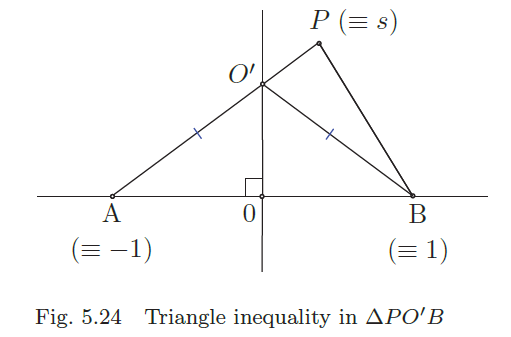
\includegraphics[width=0.5\textwidth]{./Solution/figs/fig-5-24}
\end{center}
\caption{$\Delta PO'B$에 대한 삼각부등식
}
\label{fig-5-24}
\end{figure}

그림 \ref{fig-5-24}의 $\Delta PO'B$에서 삼각부등식을 쓰면,
$\mathbb H$의 점 $s(\equiv P)$에 대하여
\begin{align*}
|s+1| = \ell(PA) = \ell(PO') + \ell(O'A)
&= \ell(PO') + \ell (O'B) \\
&> \ell(PB) = |s-1|.
\end{align*}
여기서, $O'$이 선분  $AB$의 수직이등분선임을 이용하여
세번째 등식을 얻었다.
따라서 모든 $s\in\mathbb H$에 대하여 $\varphi(s)\in \mathbb D$를 얻는다.
함수 $\varphi$가 복소해석함수임은 분명하므로, $s\in\mathbb H$에  대하여
\[
\varphi'(s) = 1\cdot \dfrac1{s+1} + (s-1)\cdot
\left( - \dfrac1{(s+1)^2} \right) = \dfrac{s+1-s+1}{(s+1)^2}
= \dfrac2{(s+1)^2}.
\]
이제 함수  $\psi: \mathbb D \to \mathbb H$를
\[
\psi(s) = \dfrac{1+z}{1-z}, \quad z\in\mathbb D
\]
로 정의하자.
($\psi$는
방정식 $z= \varphi(s) = \dfrac{s-1}{s+1}$을 $s$에 대하여 푸는 방법으로
$\varphi^{-1}$를 구한 것이다.)

\begin{figure}[h!]
\begin{center}
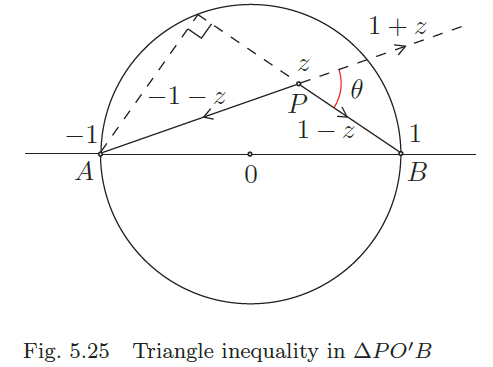
\includegraphics[width=0.5\textwidth]{./Solution/figs/fig-5-25}
\end{center}
\caption{원주각을 이용한 $\angle APB$
}
\label{fig-5-25}
\end{figure}

그림 \ref{fig-5-25}에서 원 위의 임의의 점에 대하여
지름 $AB$에 대한 원주각이 $90^\circ$이므로,
$\mathbb D$의 점 $P(\equiv z)$에 대하여
$\angle APB >90^\circ$이다. 따라서,
\[
\Re(\psi(z)) = \Re\left( \dfrac{1+z}{1-z} \right)
= |\psi(z)| \cos\theta = |\psi(z)| \cos(\pi - \angle APB) >0.
\]
따라서 모든 $z\in \mathbb D$에 대하여 $\psi(z)\in \mathbb H$이다.
함수 $\psi$는 $\mathbb D$에서 복소해석함수이고, $z\in\mathbb D$에 대하여
\[
\psi'(z) = 1\cdot \dfrac1{1-z} + (1+z)\cdot \left(\dfrac1{(1-z)^2}\right)
= \dfrac{1-z+1+z}{(1-z)^2} = \dfrac2{(1-z)^2}.
\]
끝으로, 모든 $s\in\mathbb H$에 대하여
\[
(\psi\circ \varphi)(s) = \dfrac{1+\dfrac{s-1}{s+1}}{1-\dfrac{s-1}{s+1}}
= \dfrac{s+1+s-1}{s+1-s+1} = \dfrac{2s}2 = s
\]
이고, 모든 $z\in\mathbb D$에 대하여 
\[
(\varphi\circ\psi)(z) = \dfrac{\dfrac{1+z}{1-z}-1}{\dfrac{1+z}{1-z}+1}
= \dfrac{1+z-1+z}{1+z+1-z} = \dfrac{2z}2 = z.
\]
따라서 $\varphi$는 전단사함수이고 $\varphi^{-1}=\psi$이다.


\end{itemize}


%\part{Mathematics}
%\input{./chapter/discrete_math.tex}

%=== [salt]  부록만들기
%\begin{appendices}
%\input{./chapter/appendix_formula.tex}
%\end{appendices}

\backmatter

%%%%%%%%%%%%%%% Reference %%%%%%%%%%%%%%%

\printbibliography[heading=bibintoc]
\printindex

\end{document}

